\documentclass[t]{beamer} 
\usepackage{amsmath}
\usepackage{amsthm}
\usepackage[T1]{fontenc}
\usepackage{lmodern}
\usepackage{color}
\usepackage{xcolor}
\usepackage{hyperref}
\usepackage{multirow,varwidth} % used for SL table
\usepackage{tikz}
\usepackage{multicol}
\usepackage{graphicx}
\usepackage{etoolbox}
\usepackage{bm}
\usepackage[abs]{overpic}
\usepackage{pict2e}
\usepackage{animate}
\usepackage{verbatim}
\usepackage{soul}
\usepackage{xmpmulti}
\usepackage{subfig}
\usepackage{media9}


\usetheme{PaloAlto}
\usecolortheme{seahorse}


\newenvironment{withoutheadline}{ 
\setlength{\headheight}{0pt} 
\setbeamertemplate{headline}{}}

\setbeamercolor*{block title example}{fg=white,
bg= black!30!blue}
\setbeamercolor*{block body example}{fg=black,
bg= blue!5}

\setbeamertemplate{frametitle continuation}{}

\setbeamertemplate{footline}{}

\setbeamertemplate{itemize items}[circle]
\setbeamertemplate{navigation symbols}[only frame symbol]
\setbeamerfont{framesubtitle}{size=\large}

\title{{\bf Targeted Learning (TL)}}
\subtitle{Characterizing COVID-19 Risk and its Impact on Overall Care for Immunocompromised Patients}

%\title{{\bf Targeted Learning for Characterising COVID-19 Risk  and Impact on Overall Care for Immunocompromised Patients}}
%\subtitle{Towards integration of Targa future informed by real world evidence}
\author{Mark van der Laan}


\institute{Jiann-Ping Hsu/Karl E. Peace Professor in Biostatistics \& Statistics University of California, Berkeley}

\date{August 28-29, 2023, Scientific Committee, Real World Evidence, Astrezeneca, Boston\\
%\\  AAAI-23: Bridge between Medicine and Machine Learning \\

{\tiny \vspace{5pt} Acknowledgements: Susan Gruber, Ivana Malenica and Rachael Phillips}
}

\begin{document}

\begin{frame}[noframenumbering]
\titlepage
\end{frame}
\section{Traditional Statistics}

\begin{frame}
\frametitle{Traditional toolbox for statistics: Recipe oriented, enforces false constraints, not made for Big Data}
\vspace{-12pt}
\centering
\begin{figure}
%\includegraphics[width=.75\textwidth]{statisticsForDummies.png}
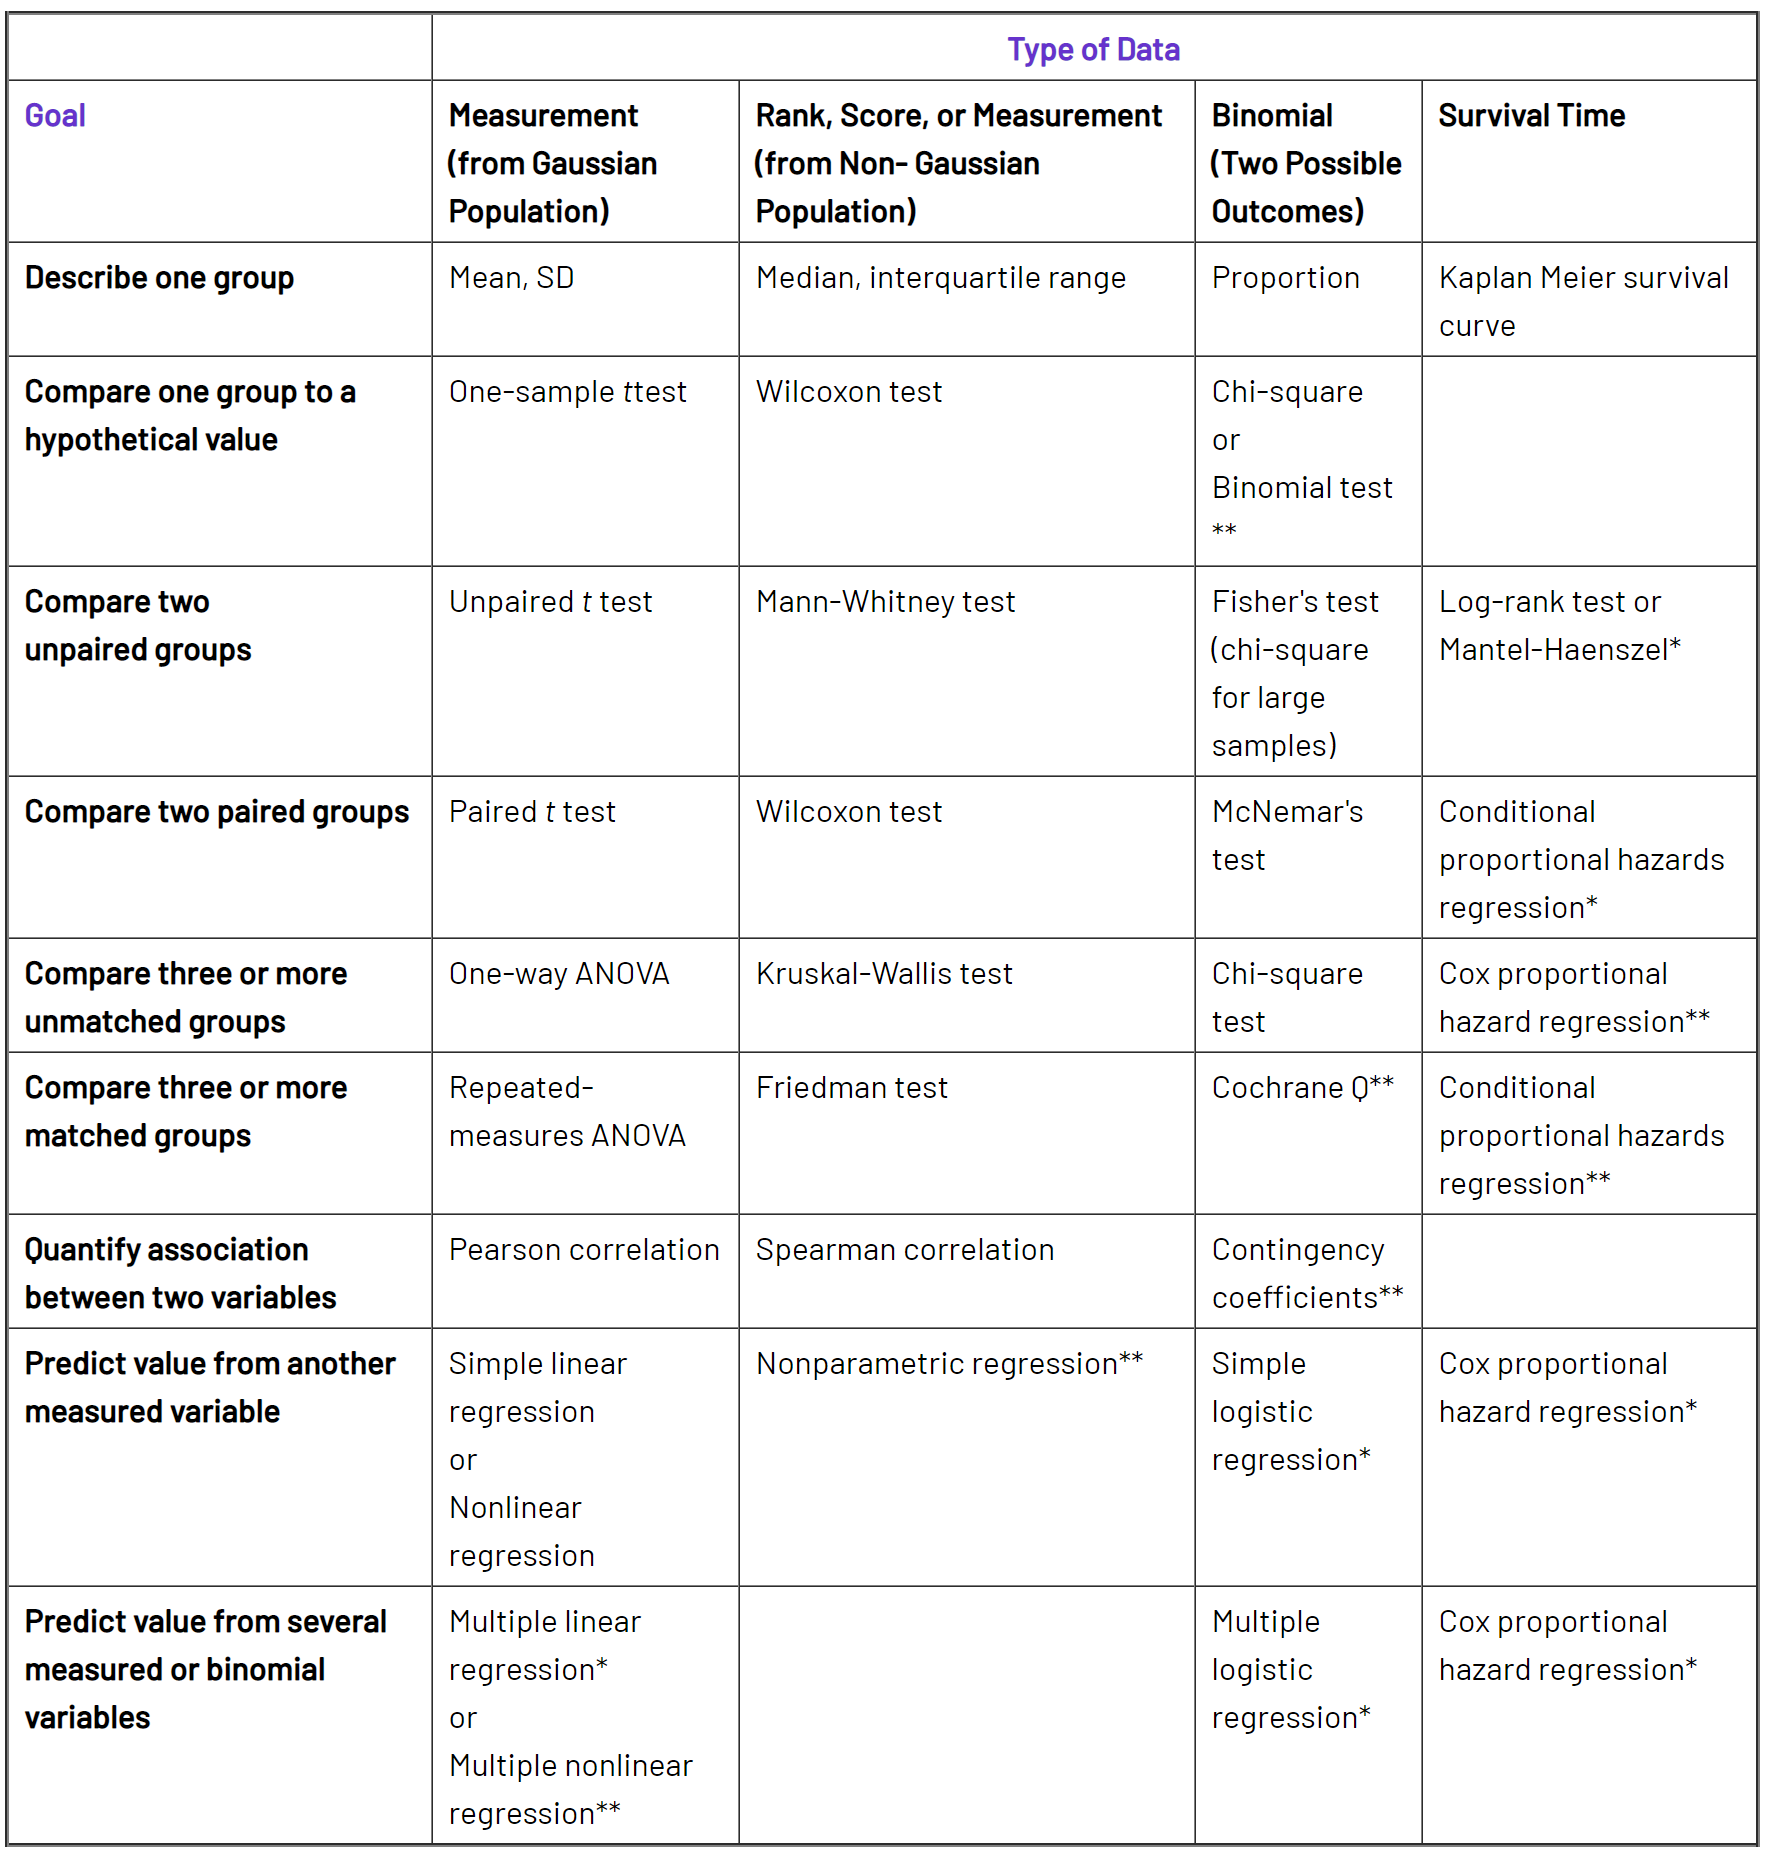
\includegraphics[width=.73\textwidth]{statistics-for-dummies.png}
% Source: https://www.graphpad.com/support/faqid/1790/
\end{figure}
\end{frame}

\begin{frame}
\frametitle{Performance of traditional tools: Coverage of Confidence Intervals deteriorates with sample size}
\vspace{5pt}
\centering
%Nima graphic n increasing, coverage to 0.
\includegraphics[width=\textwidth]{coverage_turing.pdf}
\end{frame}

\begin{frame}
\frametitle{Performance of traditional tools: Type I error deteriorates with sample size}
\vspace{5pt}
\centering
%Nima graphic n increasing, type-1 error to 1.
\includegraphics[width=\textwidth]{error_turing.pdf}
\end{frame}

\begin{frame}
\frametitle{Traditional tools invite/encourage post-hoc model manipulation}
\centering
\vspace{-.11in}
\begin{figure}
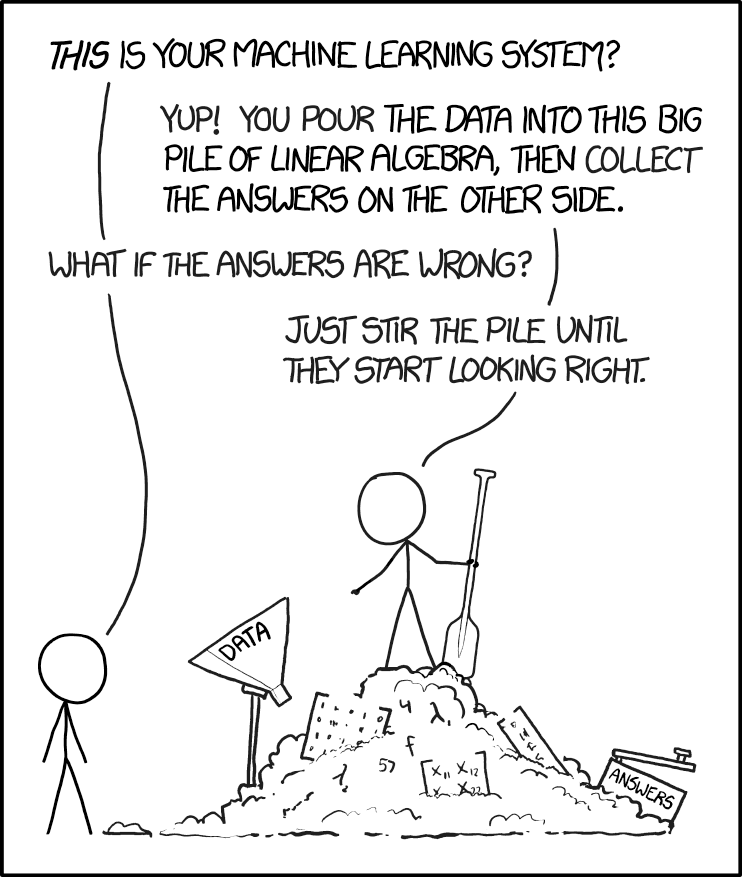
\includegraphics[width=0.62\textwidth]{comic.png}
\end{figure}
\end{frame}

\begin{frame}
\frametitle{Why care about statistical inference?}
\vspace{-.2in}
\centering
\begin{figure}
\fbox{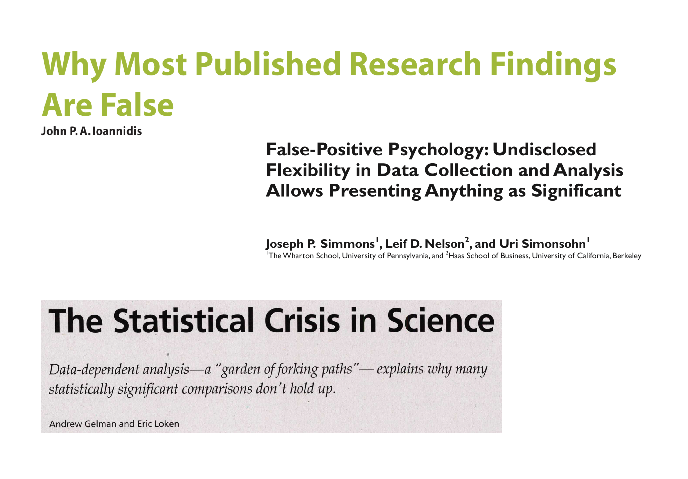
\includegraphics[width=.99\textwidth]{articles.pdf}}
\end{figure}
\end{frame}

%\begin{frame}
%\frametitle{Expectations vs. Reality: What are we actually estimating?}
%\centering
%\begin{figure}
%\includegraphics[width=1.03\textwidth]{538graphic.png}
%\end{figure}
%\end{frame}

%The challenge facing modern statisticians (and you, as students in this %class) is how to develop statistical methods aimed at answering specific %scientific questions of interest, while utilizing state-of-the-art %algorithms.

\section{Overview TL}

\begin{frame}
  \frametitle{Targeted Learning for answering statistical and causal questions with confidence intervals}
  \vspace{-1em}
  \begin{center}
  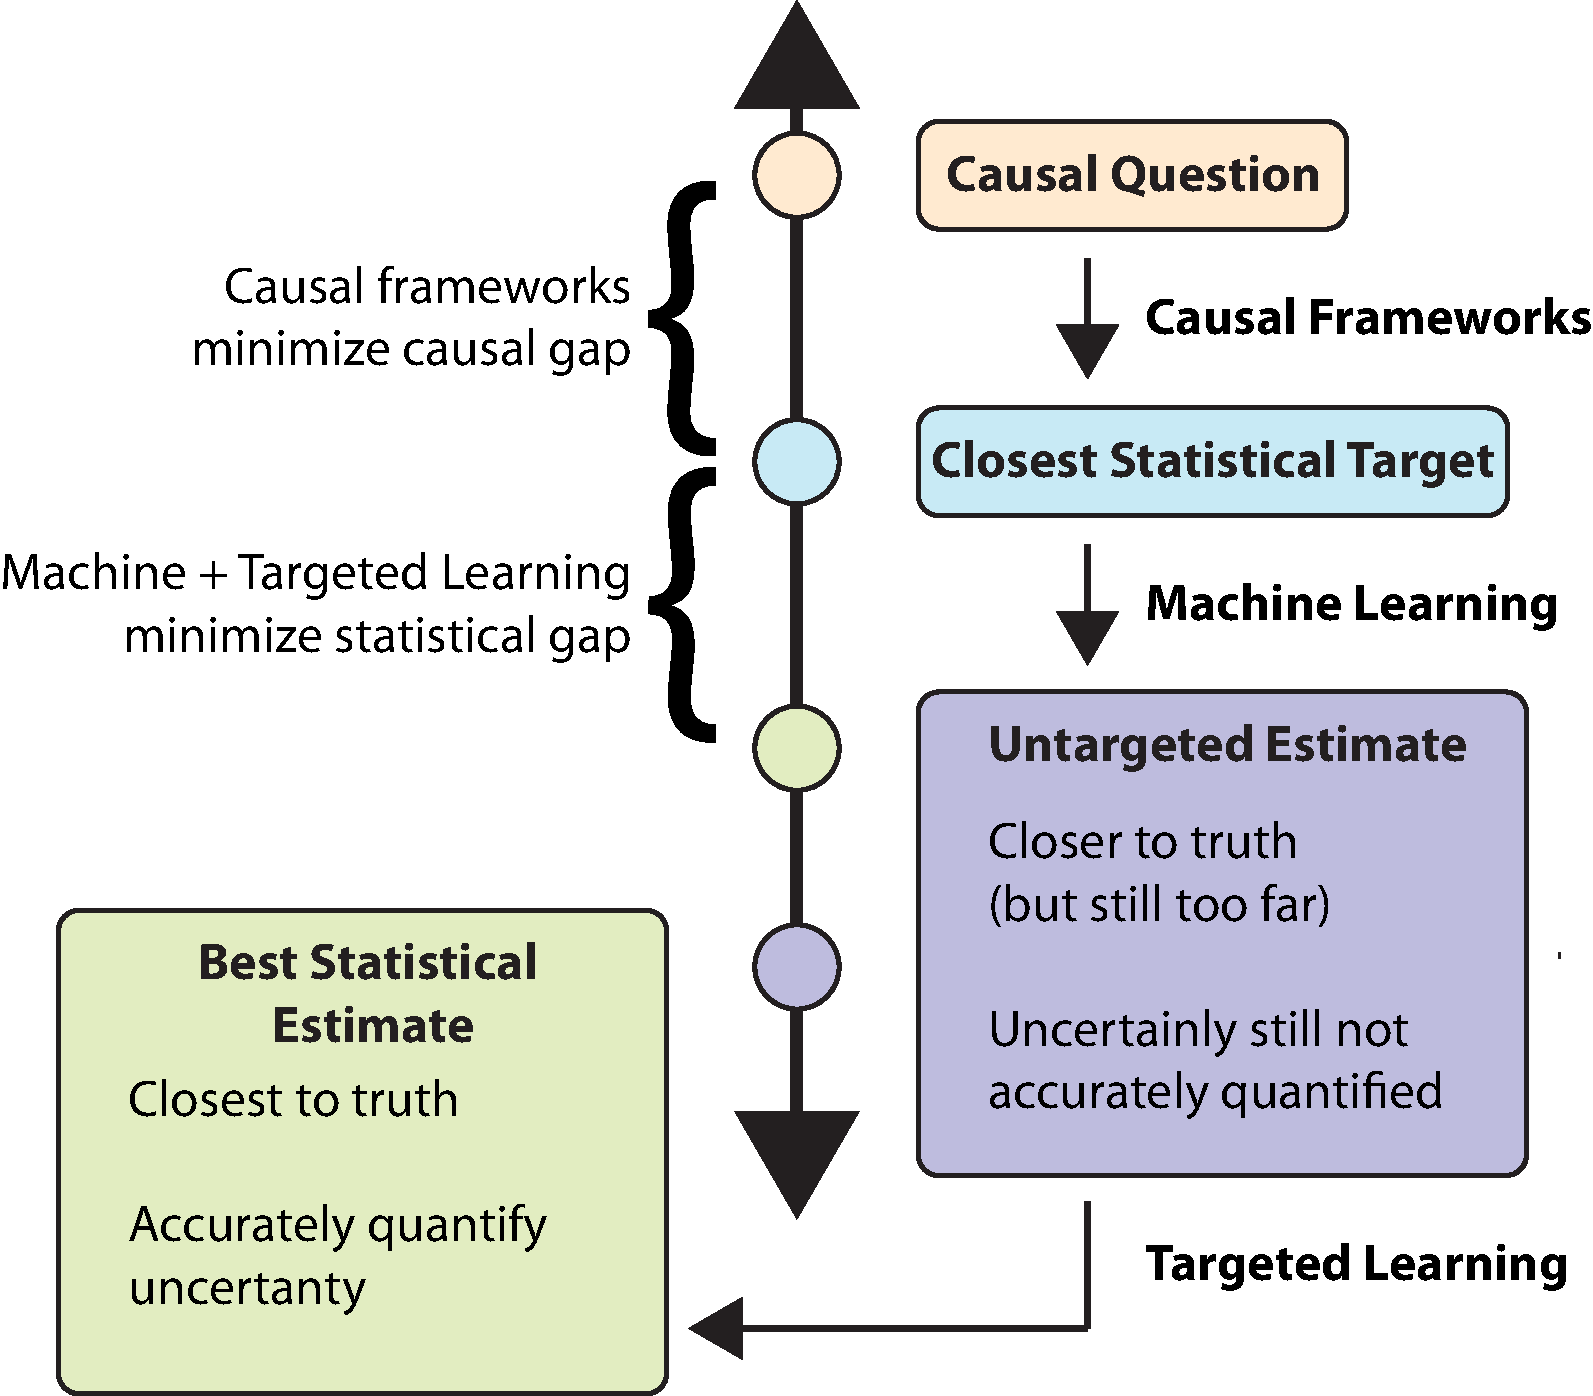
\includegraphics[width=.84\textwidth]{schematic.pdf}
  \end{center}
\end{frame}
%\begin{frame}\frametitle{Targeted Learning is a subfield of statistics}\vspace{-25pt}\begin{columns}\begin{column}{4.9cm}\begin{center}\begin{figure}\fbox{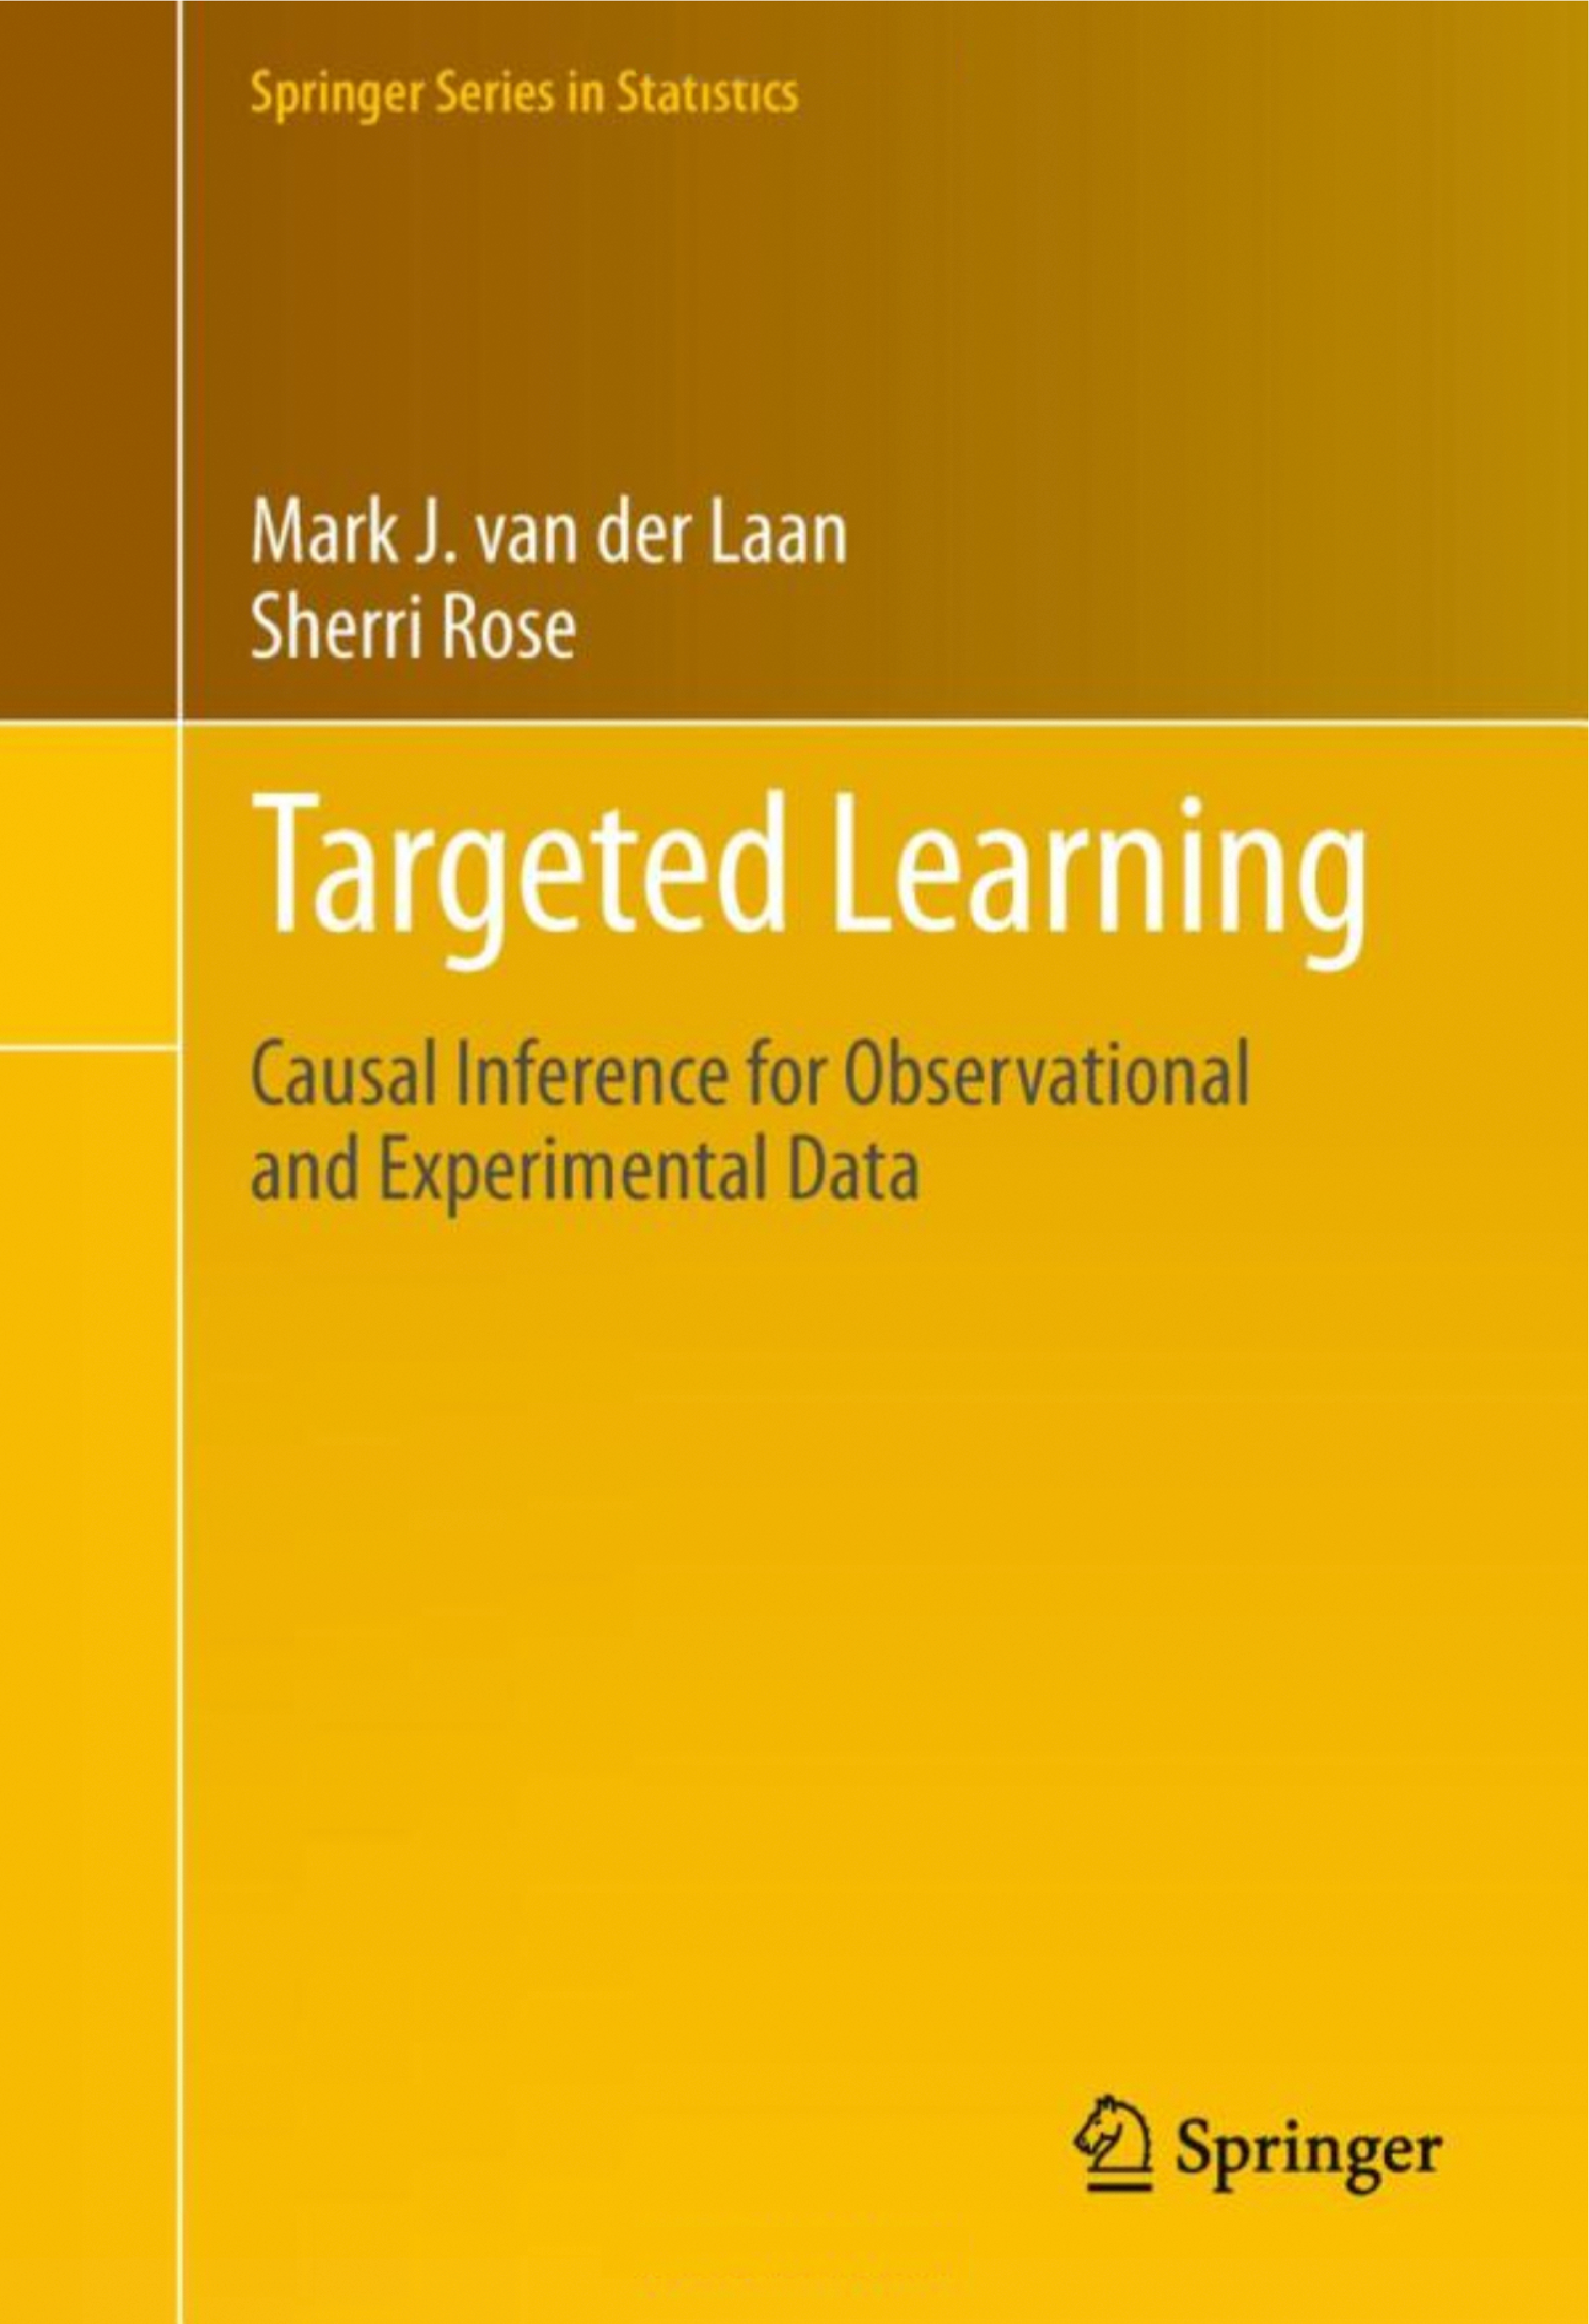
\includegraphics[height=1.7in]{2011Book.pdf}}\end{figure}\end{center}\end{column}\begin{column}{4.9cm}\begin{figure}\fbox{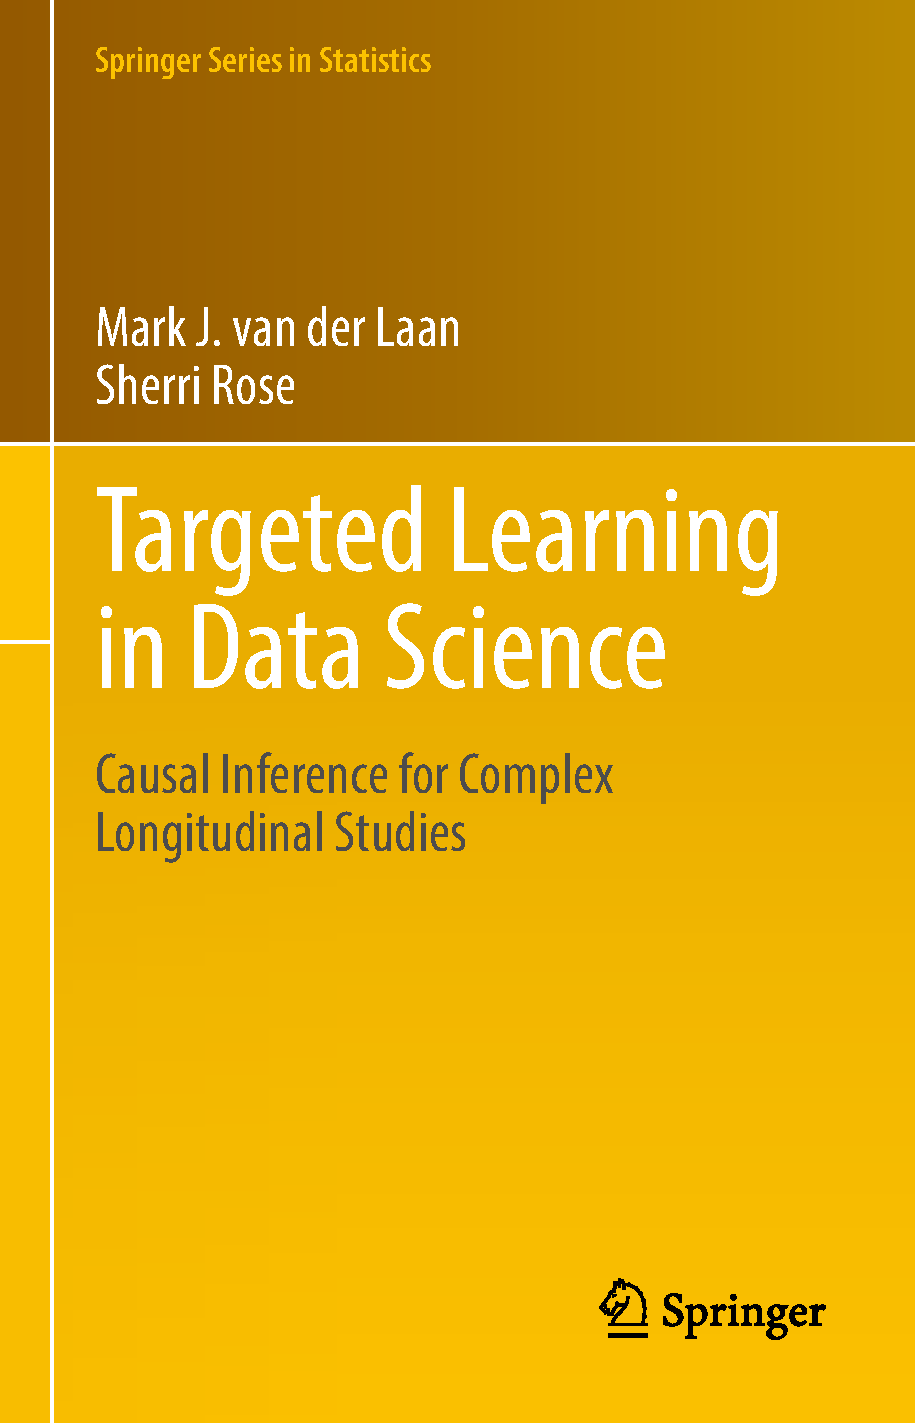
\includegraphics[height=1.7in]{2018Book.pdf}}\end{figure}\end{column}\end{columns}\vspace{-10pt}\begin{columns}\begin{column}{4.9cm}\begin{center}{\footnotesize van der Laan \& Rose, \textit{Targeted Learning: Causal Inference for Observational and Experimental Data}. New York: Springer, 2011.}\end{center}\end{column}\begin{column}{4.9cm}\begin{center}{\footnotesize van der Laan \& Rose, \textit{Targeted Learning in Data Science: Causal Inference for Complex Longitudinal Studies}. New York: Springer, 2018.}\end{center}\end{column}\end{columns}\vspace{15pt}\centering
% \href{https://vanderlaan-lab.org}{https://vanderlaan-lab.org} \hspace{10mm} \href{https://tlverse.org/tlverse-handbook/}{The Hitchhiker’s Guide to the \texttt{tlverse}}\end{frame}

%\begin{frame}\frametitle{Better clinical decisions from observational data}\vspace{-20pt}\begin{center}  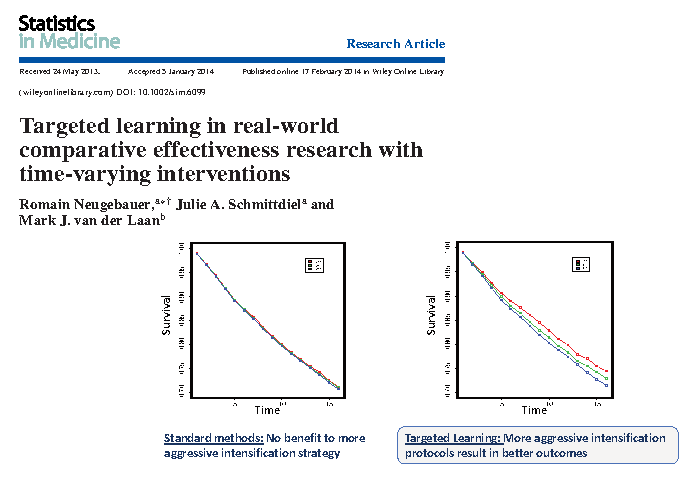
\includegraphics[width = 1.02\textwidth]{diabetes.pdf}  \end{center}\end{frame}



\section{Challenges with RWD}

\begin{frame}
\frametitle{Statistical challenges with RWD}
\vspace{20pt}
\begin{center}
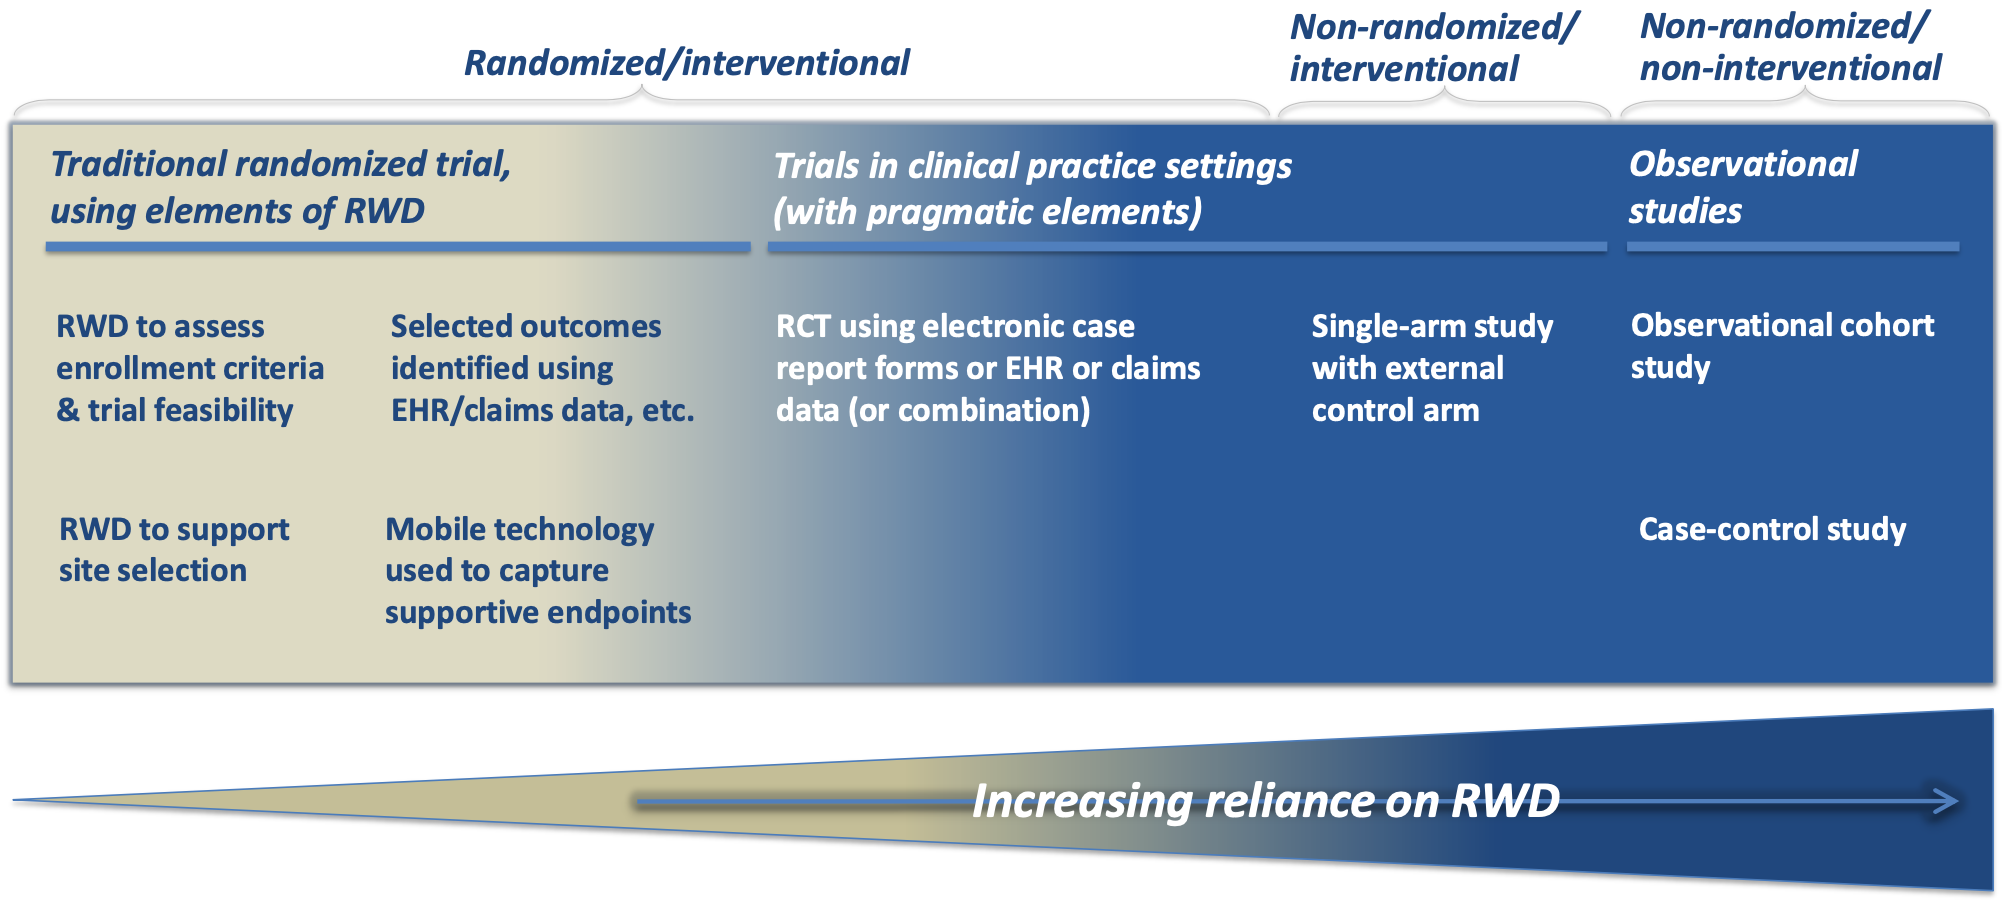
\includegraphics[width=\textwidth]{figures/john_slide8_figure.png}
\end{center}
\vspace{35pt}
\tiny{Courtesy of "FDA Real-World Evidence Program" Webinar by John Concato on 4 August 2021}
\end{frame}

\begin{frame}
\frametitle{Statistical challenges with RWD}
\vspace{-18pt}
\begin{center}
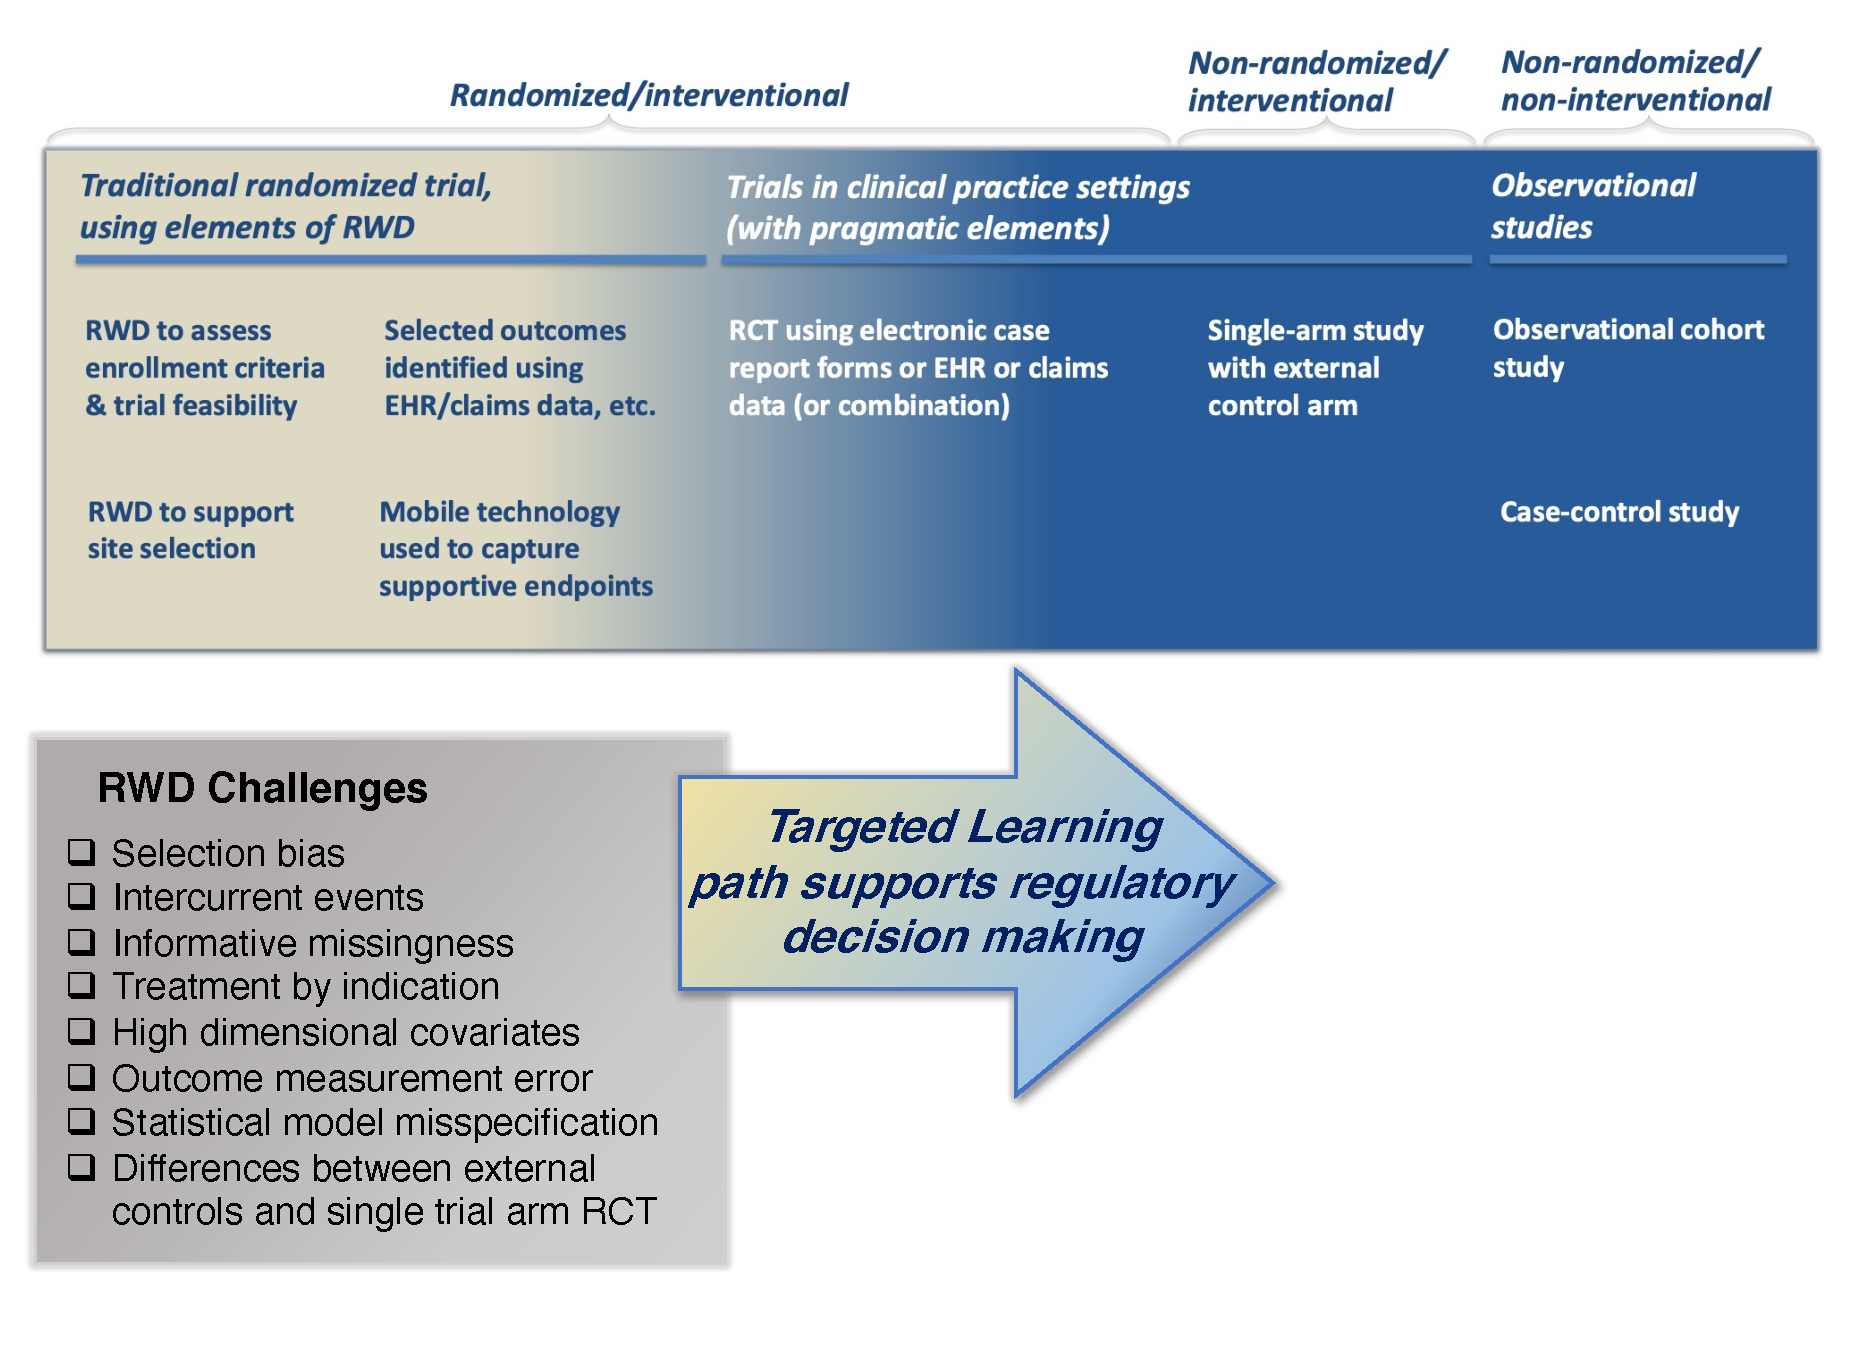
\includegraphics[width=1.02\textwidth]{figures/TLpath1_edit.pdf}
\end{center}
\end{frame}
\section{Interest in TL for FDA RWE}
\begin{frame}\frametitle{Interest in Targeted Learning by FDA RWE program and Pharma}
\begin{itemize}
\item Targeted Learning one of demonstration projects (2 years) of FDA RWE Program.
\item Sentinel Innovation Center running various projects concerning Targeted Learning Tool Development and demonstrations in safety analysis. 
\item Growing interest from Pharma and FDA (e.g., workshop training FDA reviewers) about RWE SAP development based on TL. 
\item Lots of open source software (e.g., TLverse in R). 
\item General agreement on setting standards for generating RWE under FDA regulatory guidance: Forum for Integration of Observational and Randomized Data (CTML), 2022, resulting in general consensus roadmap paper and case-study papers, by FDA/Pharma/Academic representatives.
\end{itemize}
\end{frame}

\section{TL Roadmap}

\begin{frame}
  \frametitle{The roadmap for causal inference}
  \vspace{-20pt}
  \begin{center}
  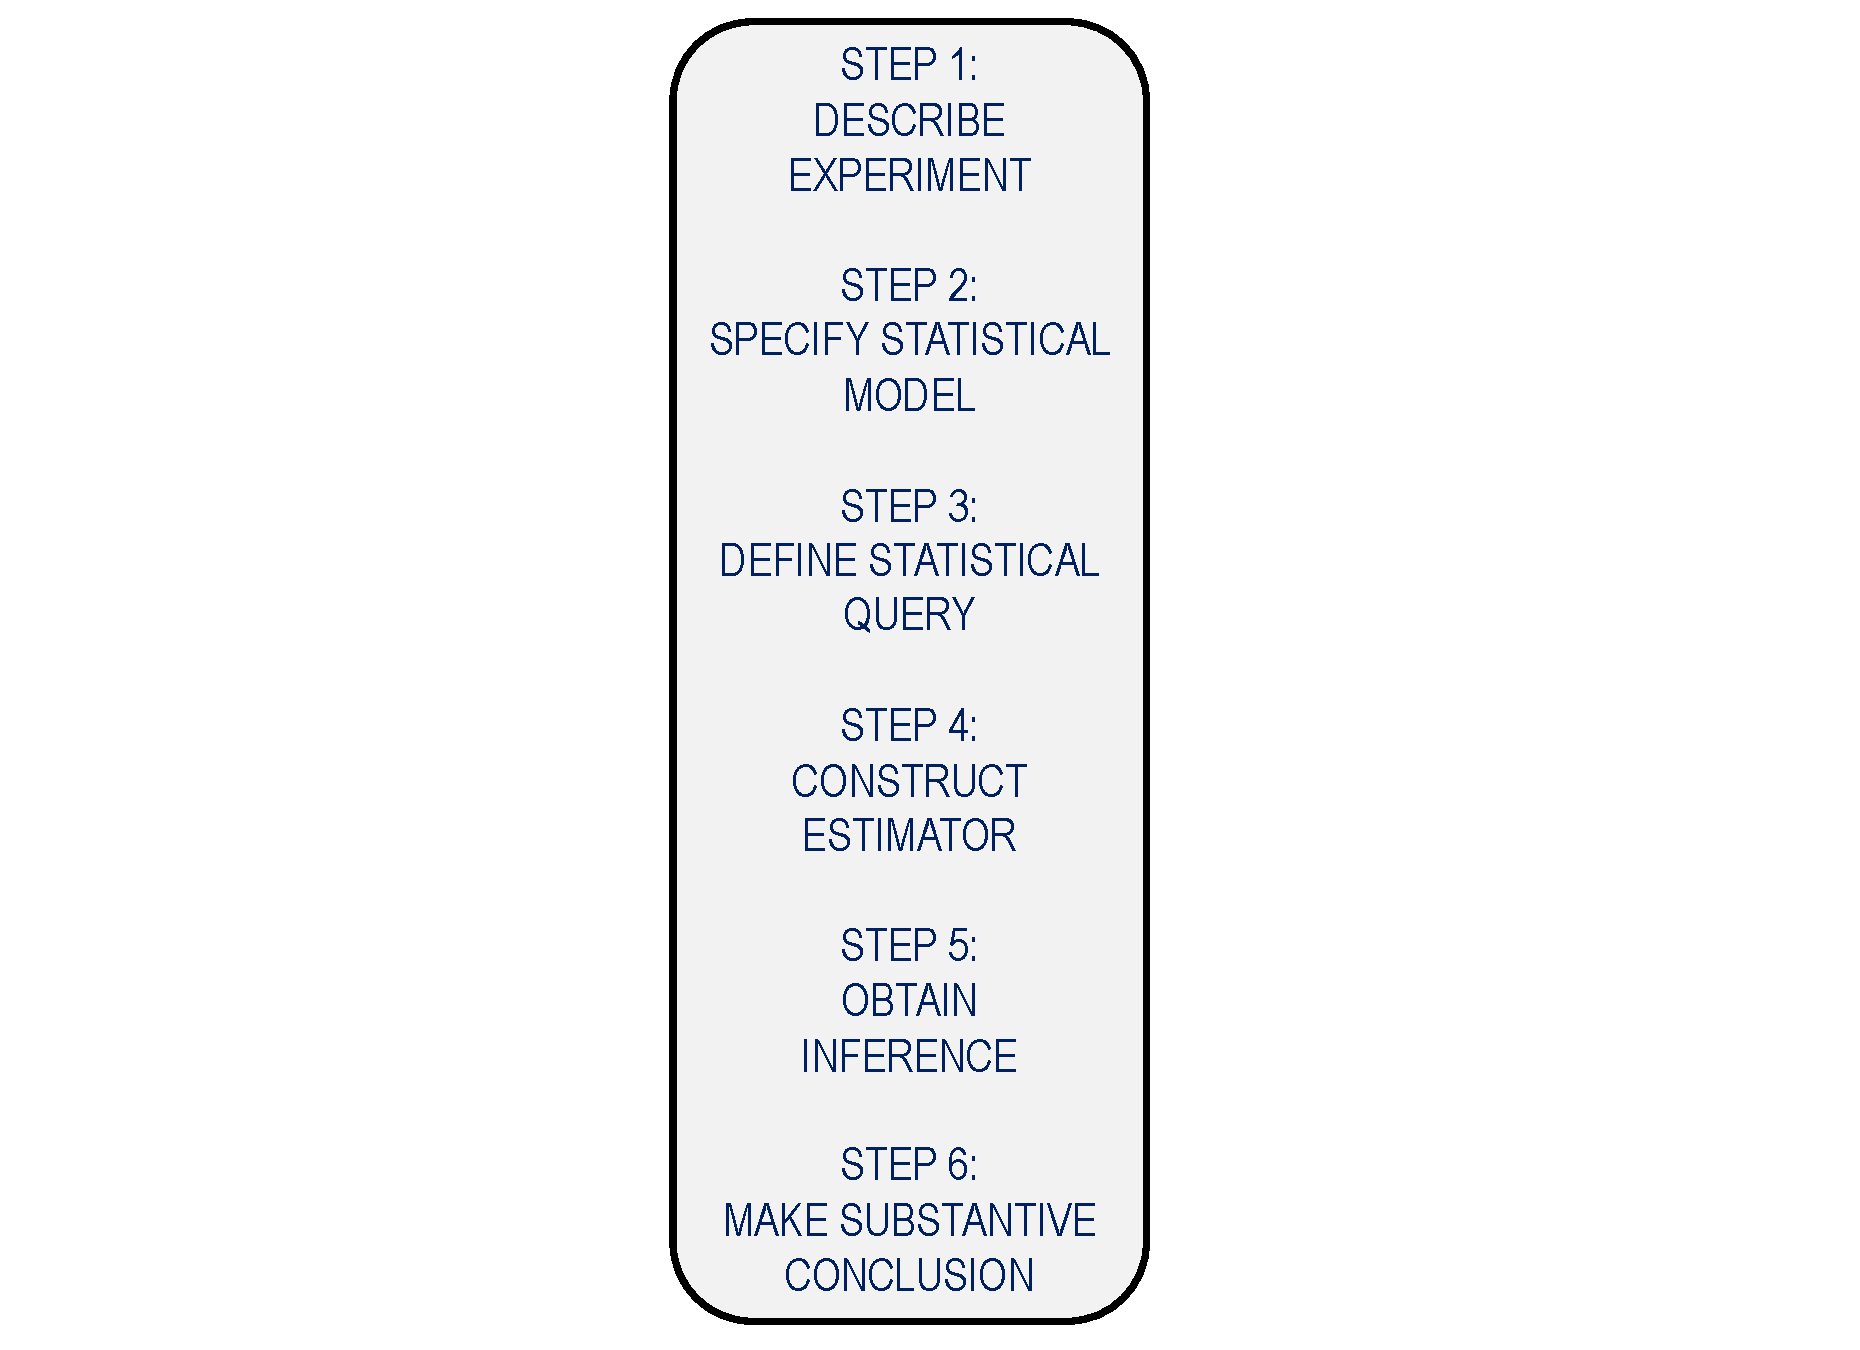
\includegraphics[width = 1.05\textwidth]{figures/roadmap.pdf}
  \end{center}
\end{frame}

%\subsection{Describe experiment/study}
\begin{frame}
  \frametitle{What is the experiment that generated the data?}
  \vspace{-20pt}
  \begin{center}
  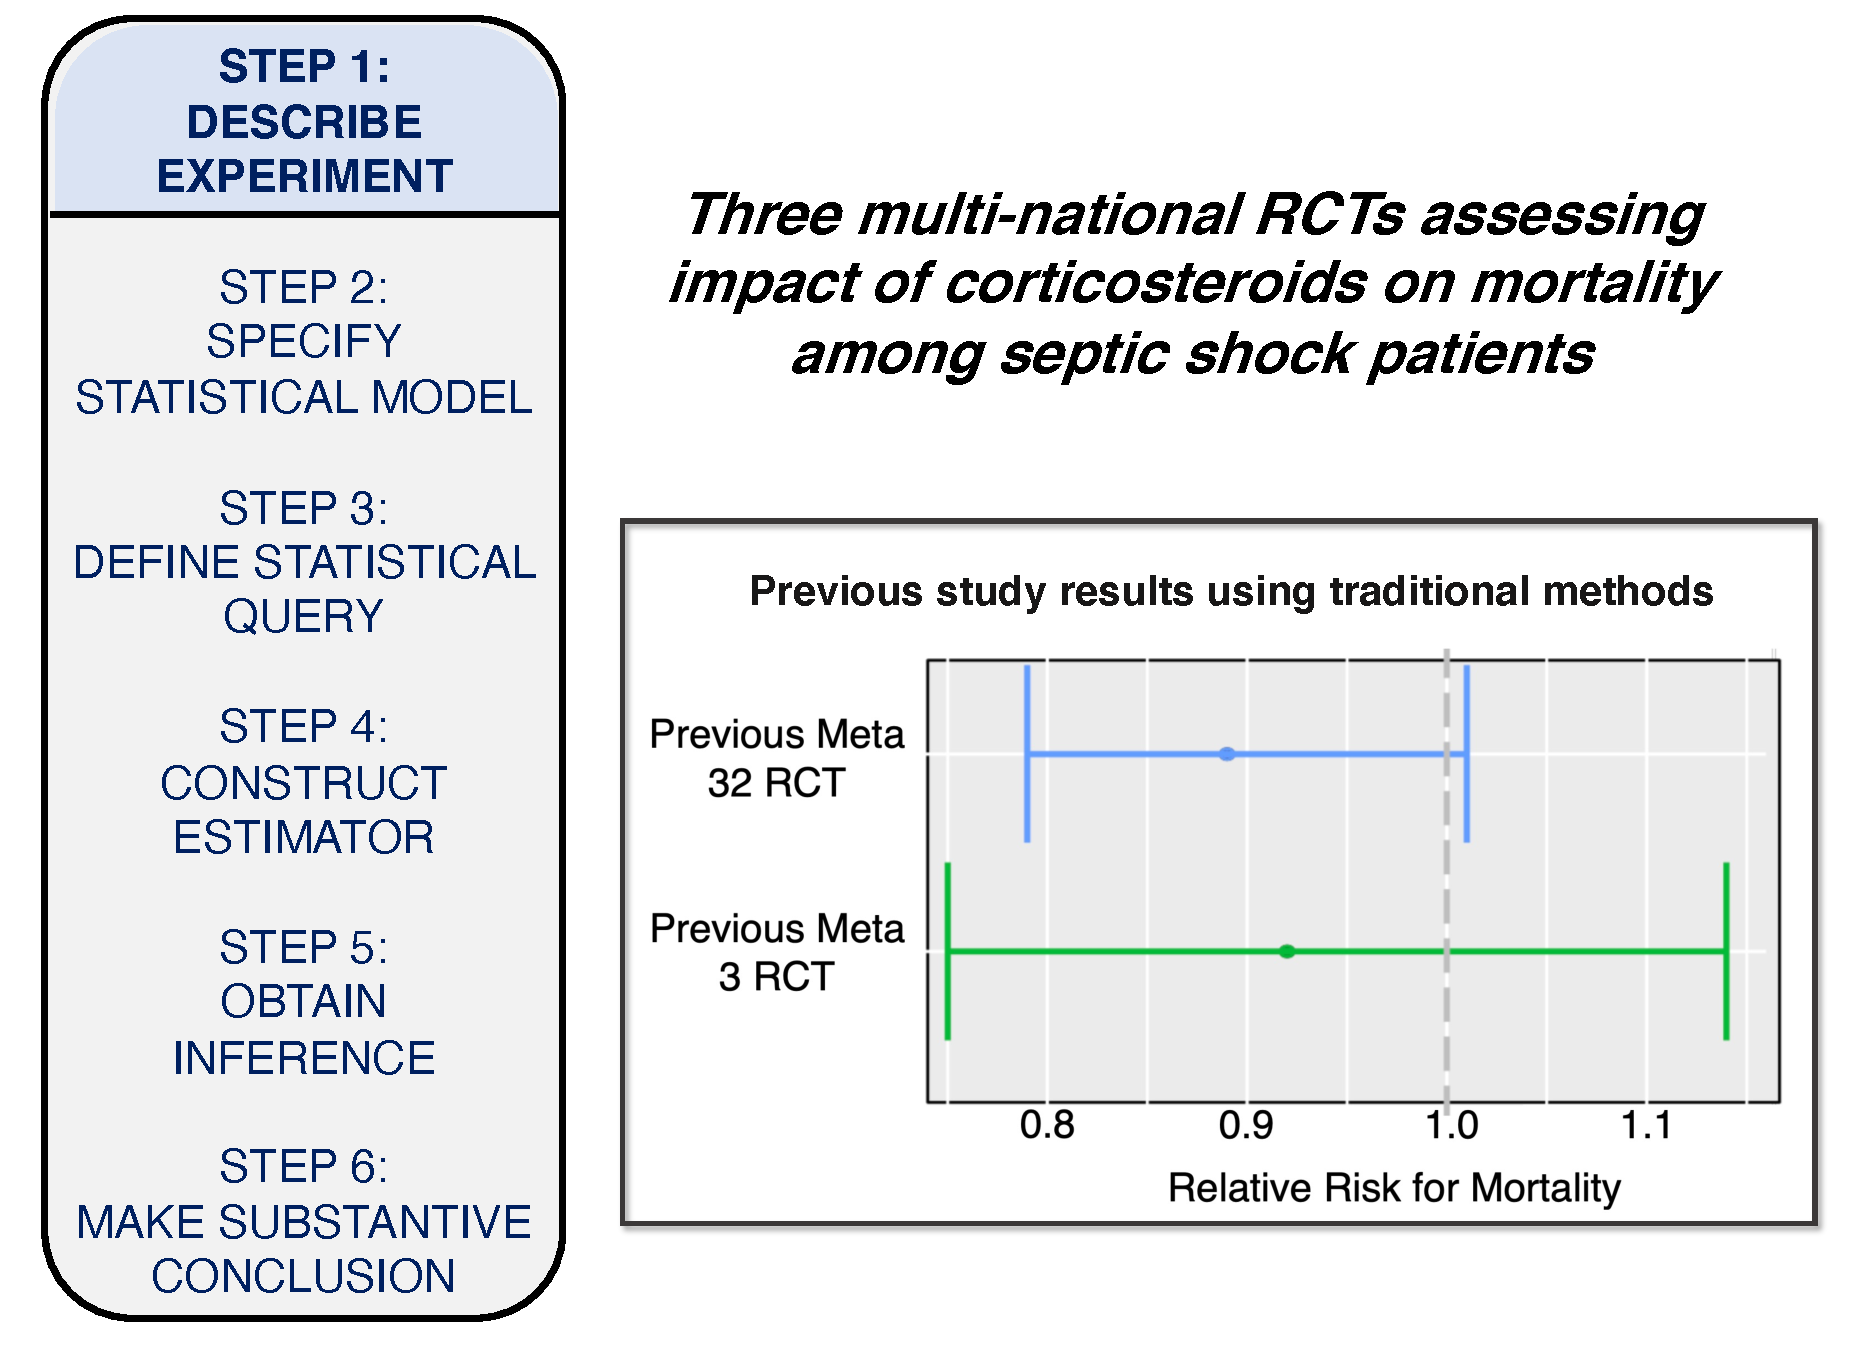
\includegraphics[width = 1.05\textwidth]{figures/roadmap1_1.pdf}
  \end{center}
\end{frame}

\begin{frame}
  \frametitle{What is the experiment that generated the data?}
  \vspace{-20pt}
  \begin{center}
  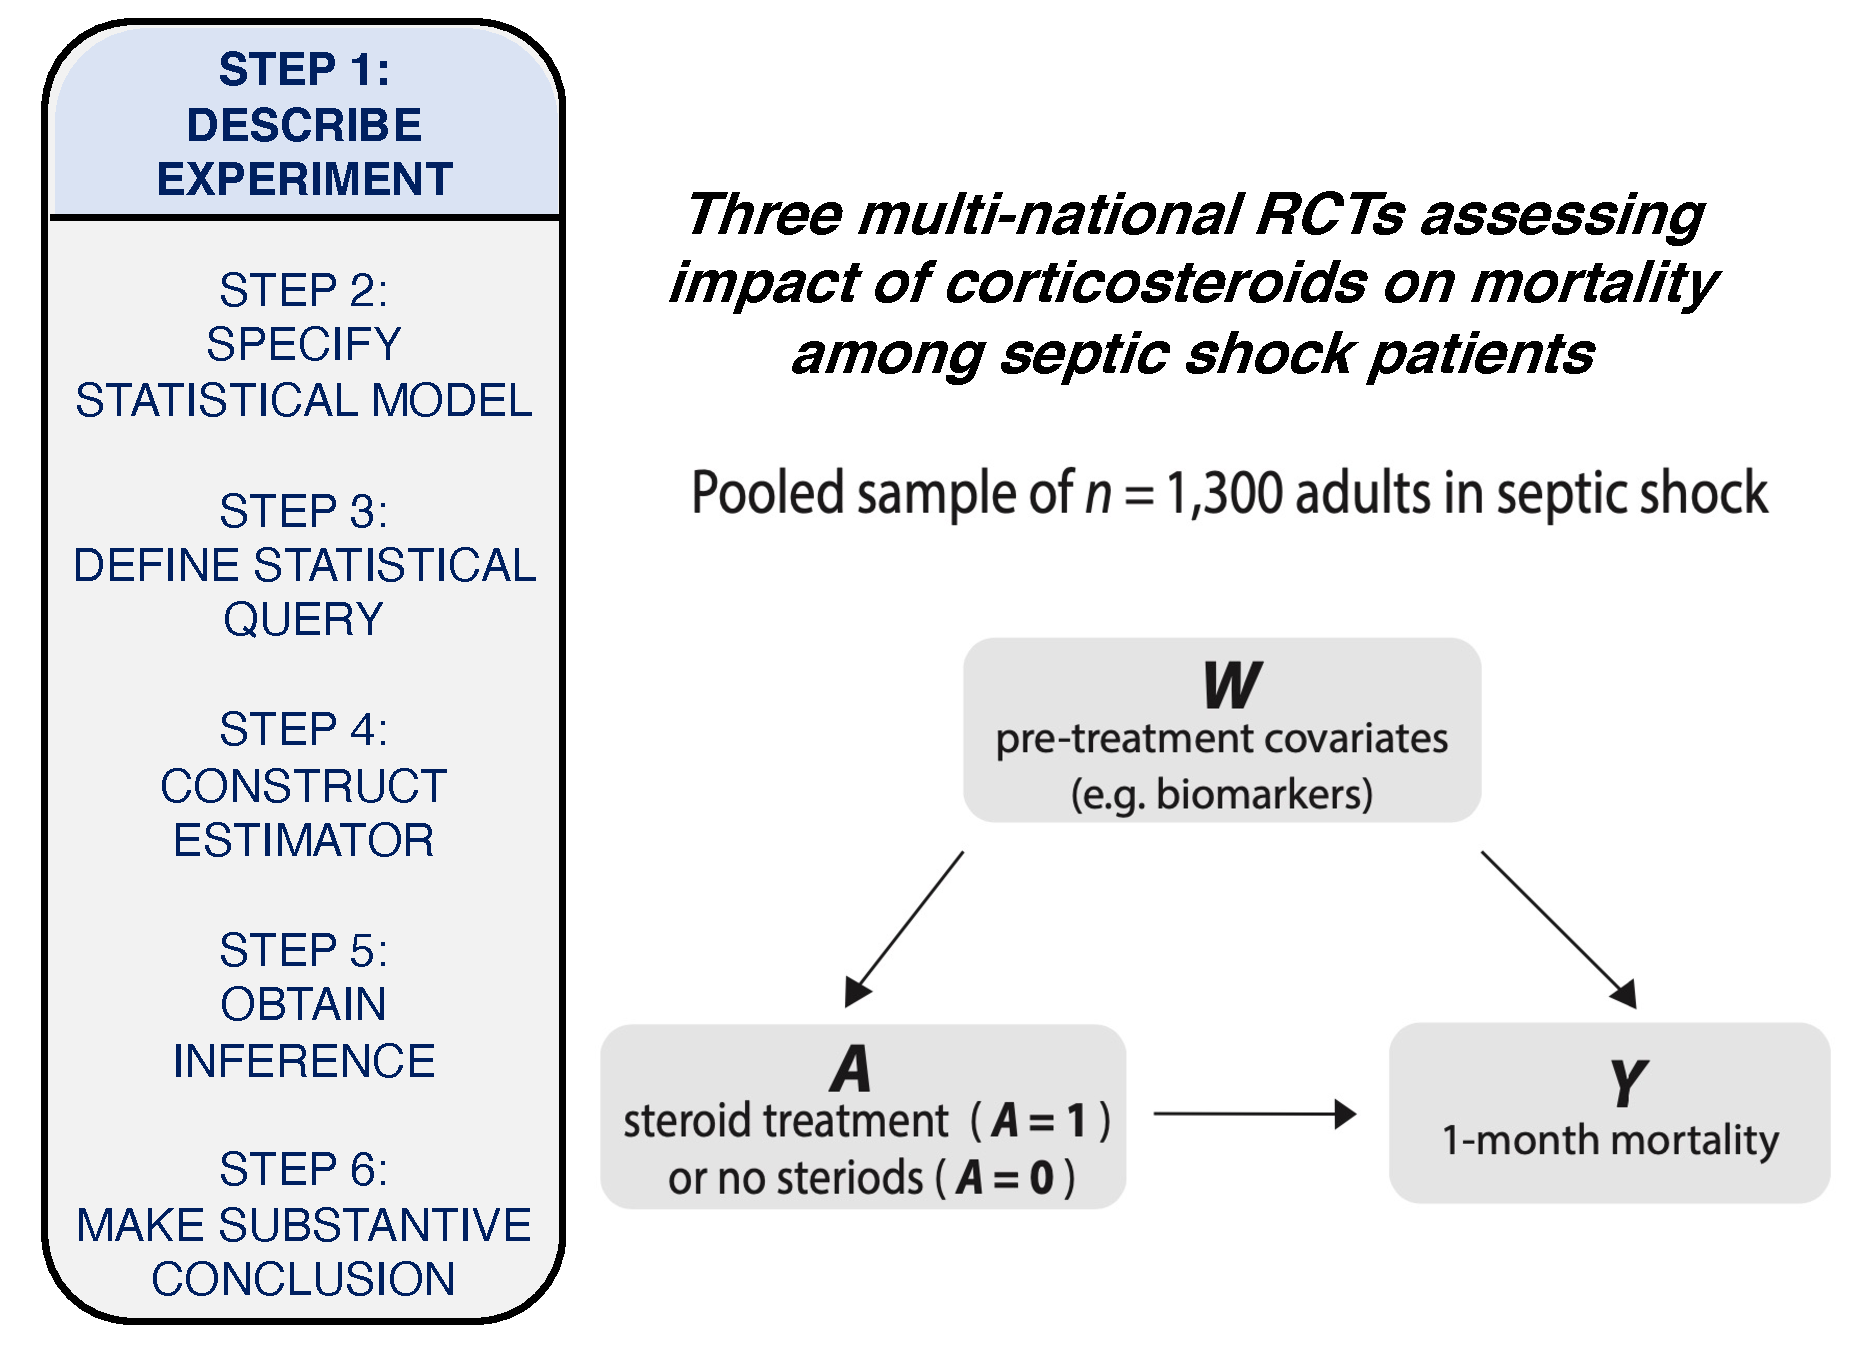
\includegraphics[width = 1.05\textwidth]{figures/roadmap1_2.pdf}
  \end{center}
\end{frame}


%\subsection{Specify realistic statistical model}
\begin{frame}
  \frametitle{What is known about stochastic relations of the observed variables?}
  \vspace{-20pt}
  \begin{center}
  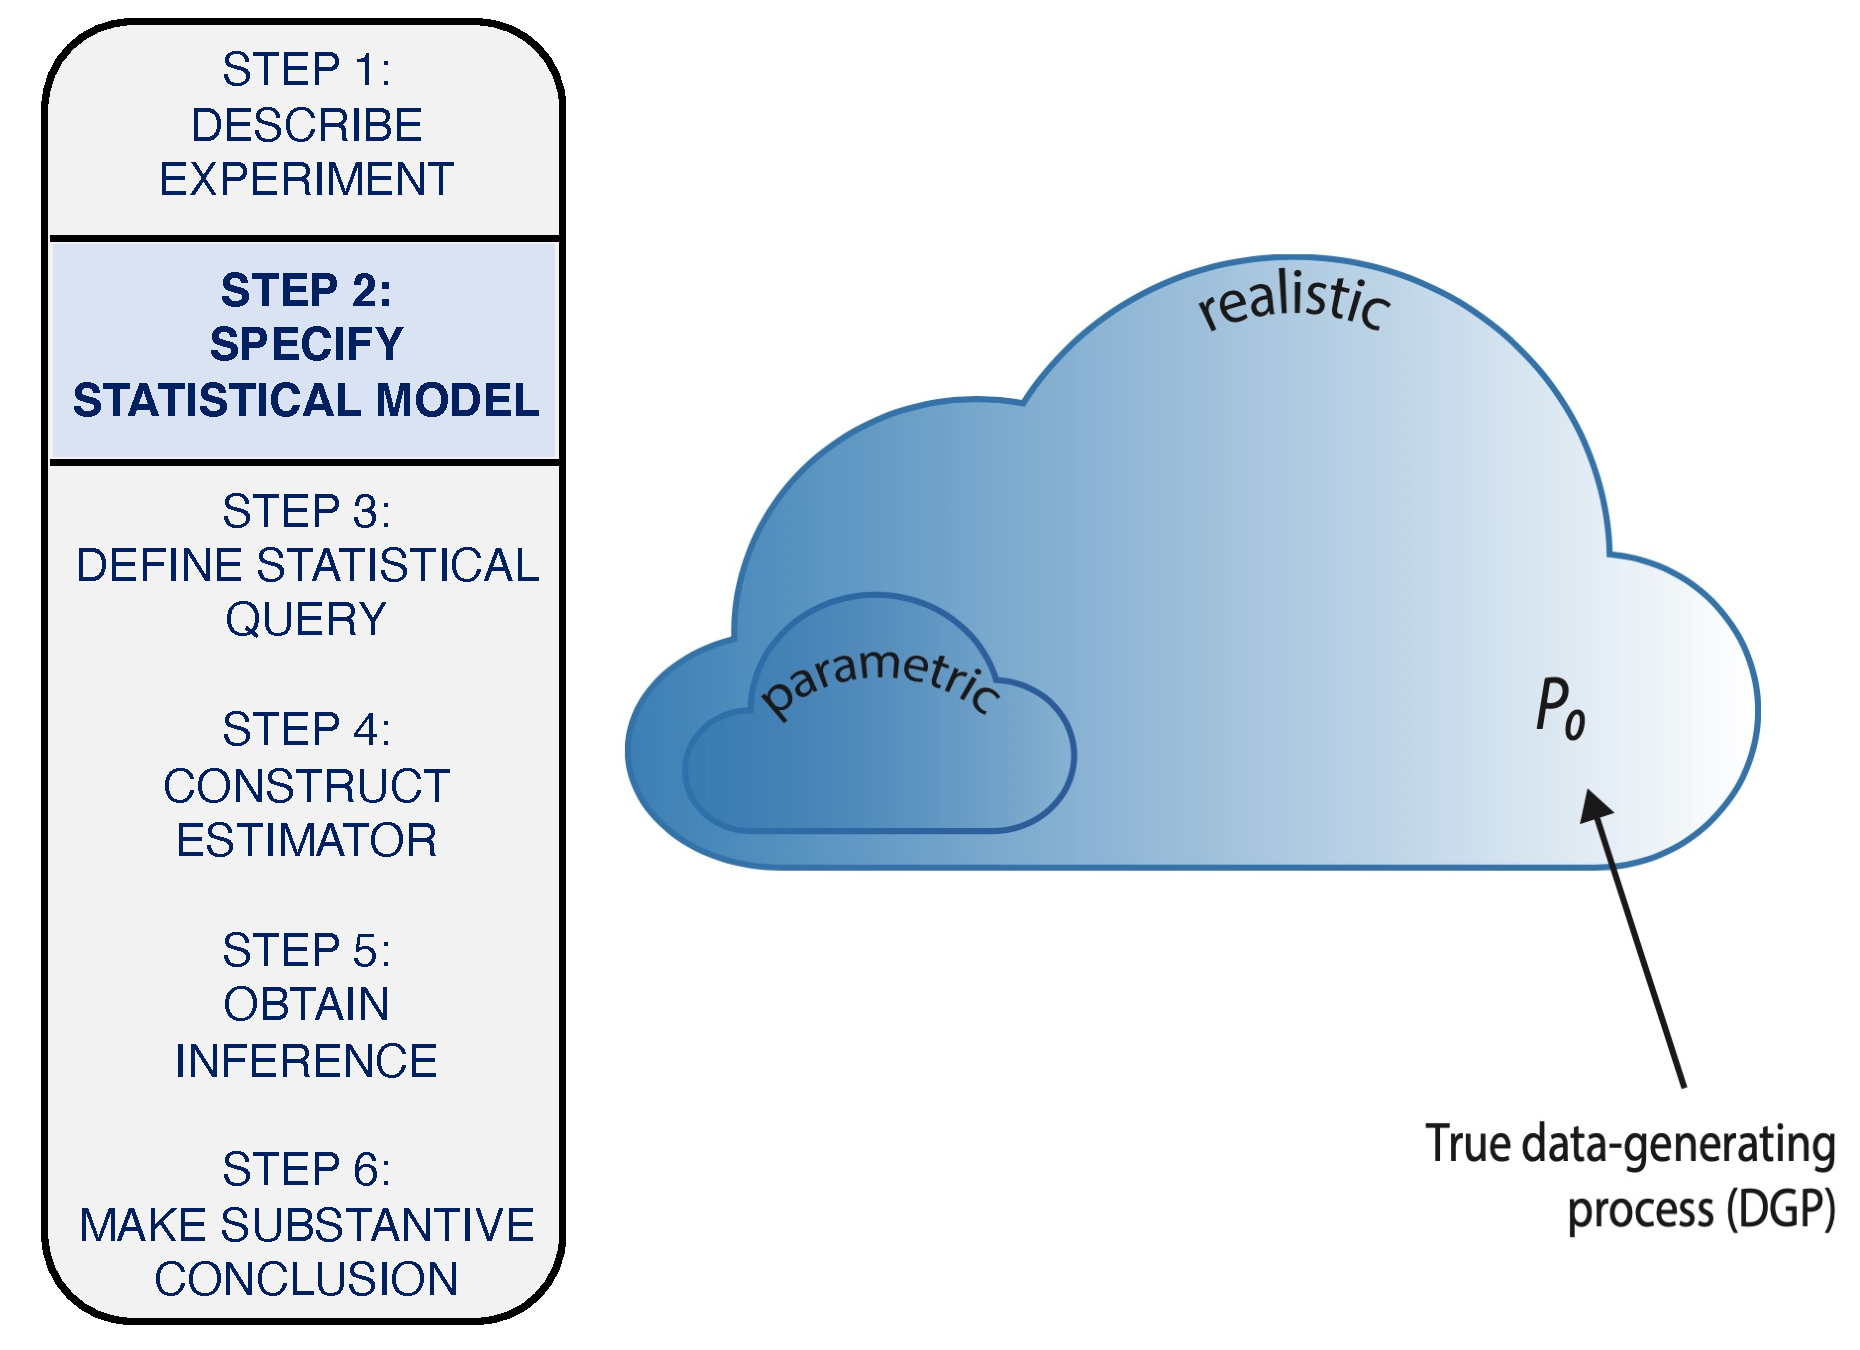
\includegraphics[width = 1.05\textwidth]{figures/roadmap2.pdf}
  \end{center}
\end{frame}

\begin{frame}
\frametitle{What happens when the statistical model is misspecified and does not contain the DGP?}
\vspace{15pt}
\centering
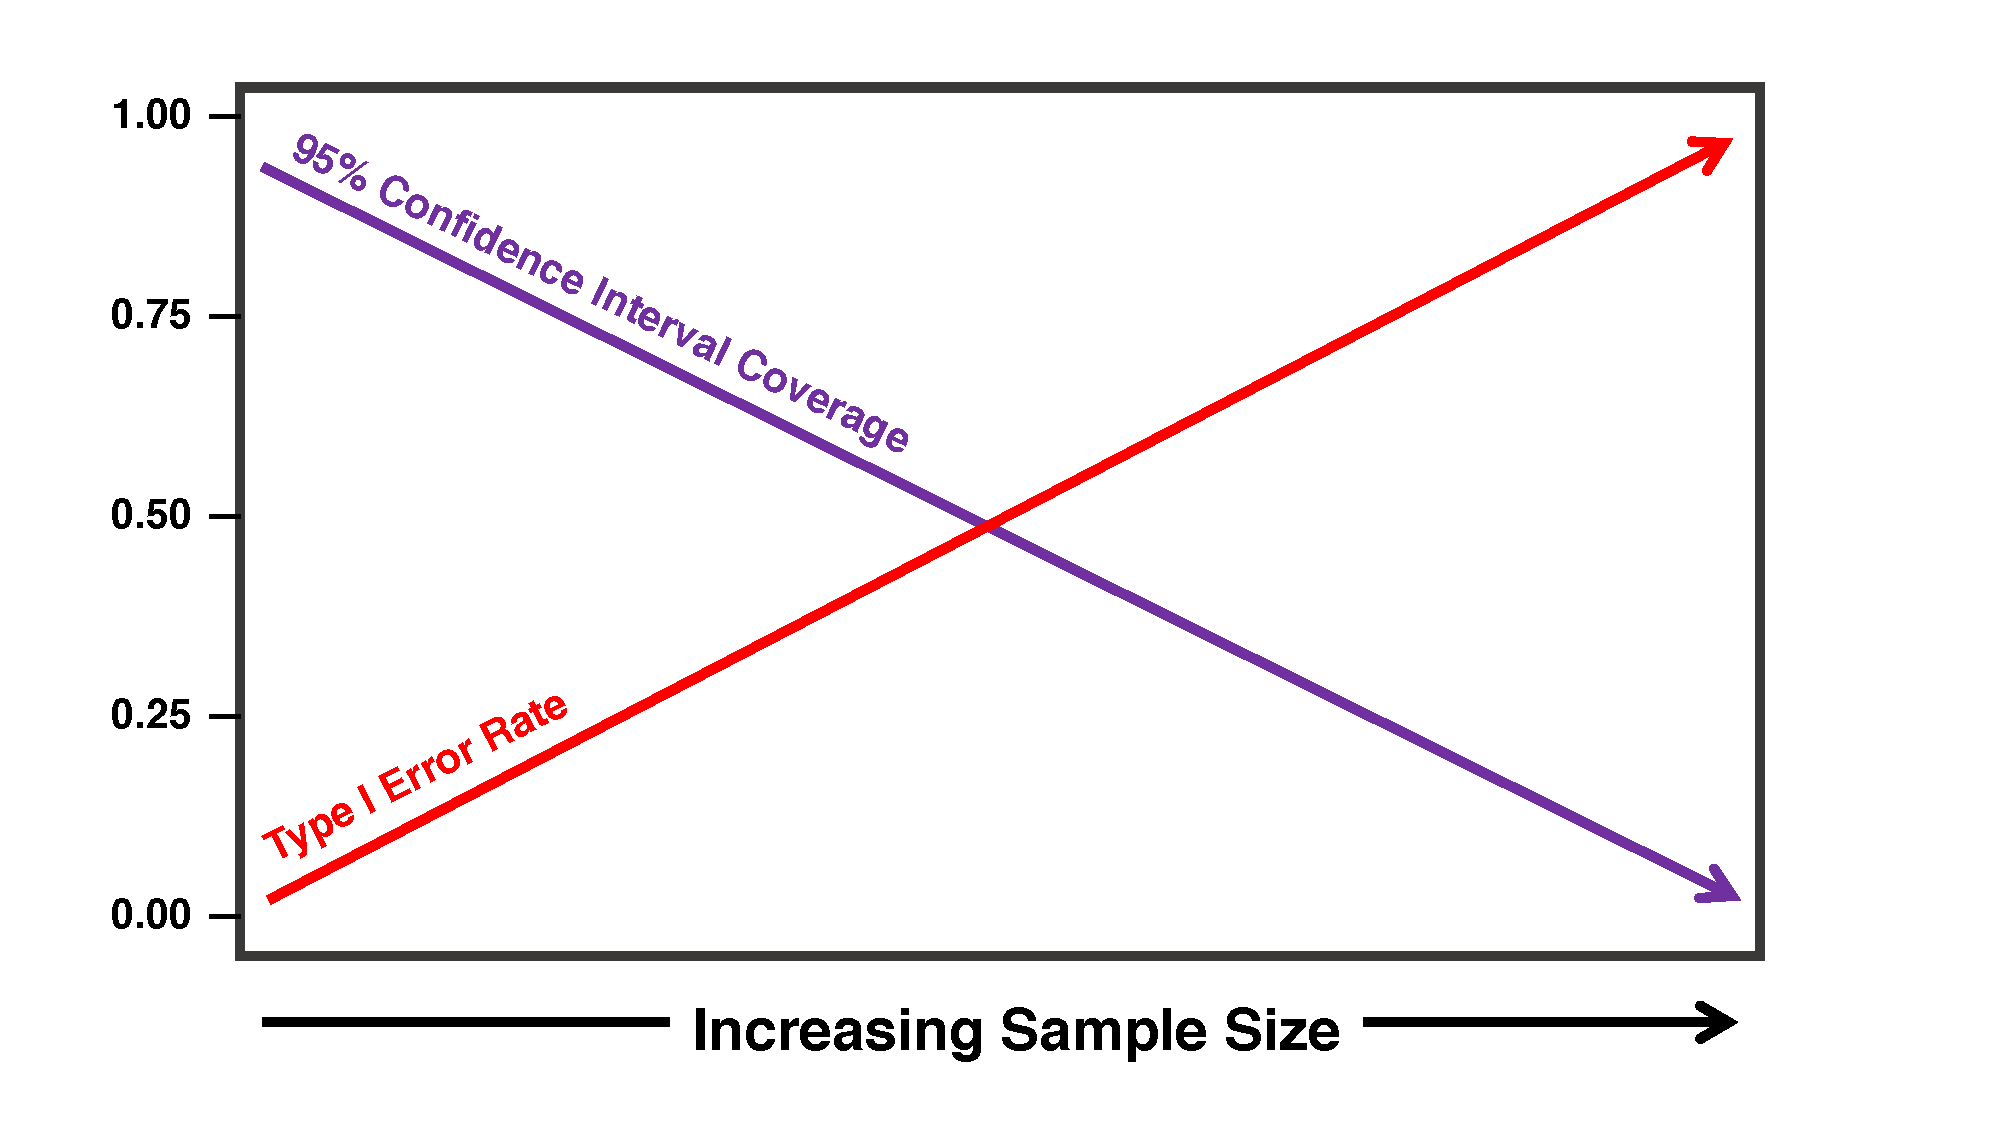
\includegraphics[width=1.05\textwidth]{figures/misspecified.pdf}
\end{frame}

%\subsection{Define statistical estimand}
\begin{frame}
  \frametitle{Step 3a: What is the target causal estimand that we aim to identify from the data?}
  % defining full-data
  \vspace{-20pt}
  \begin{center}
  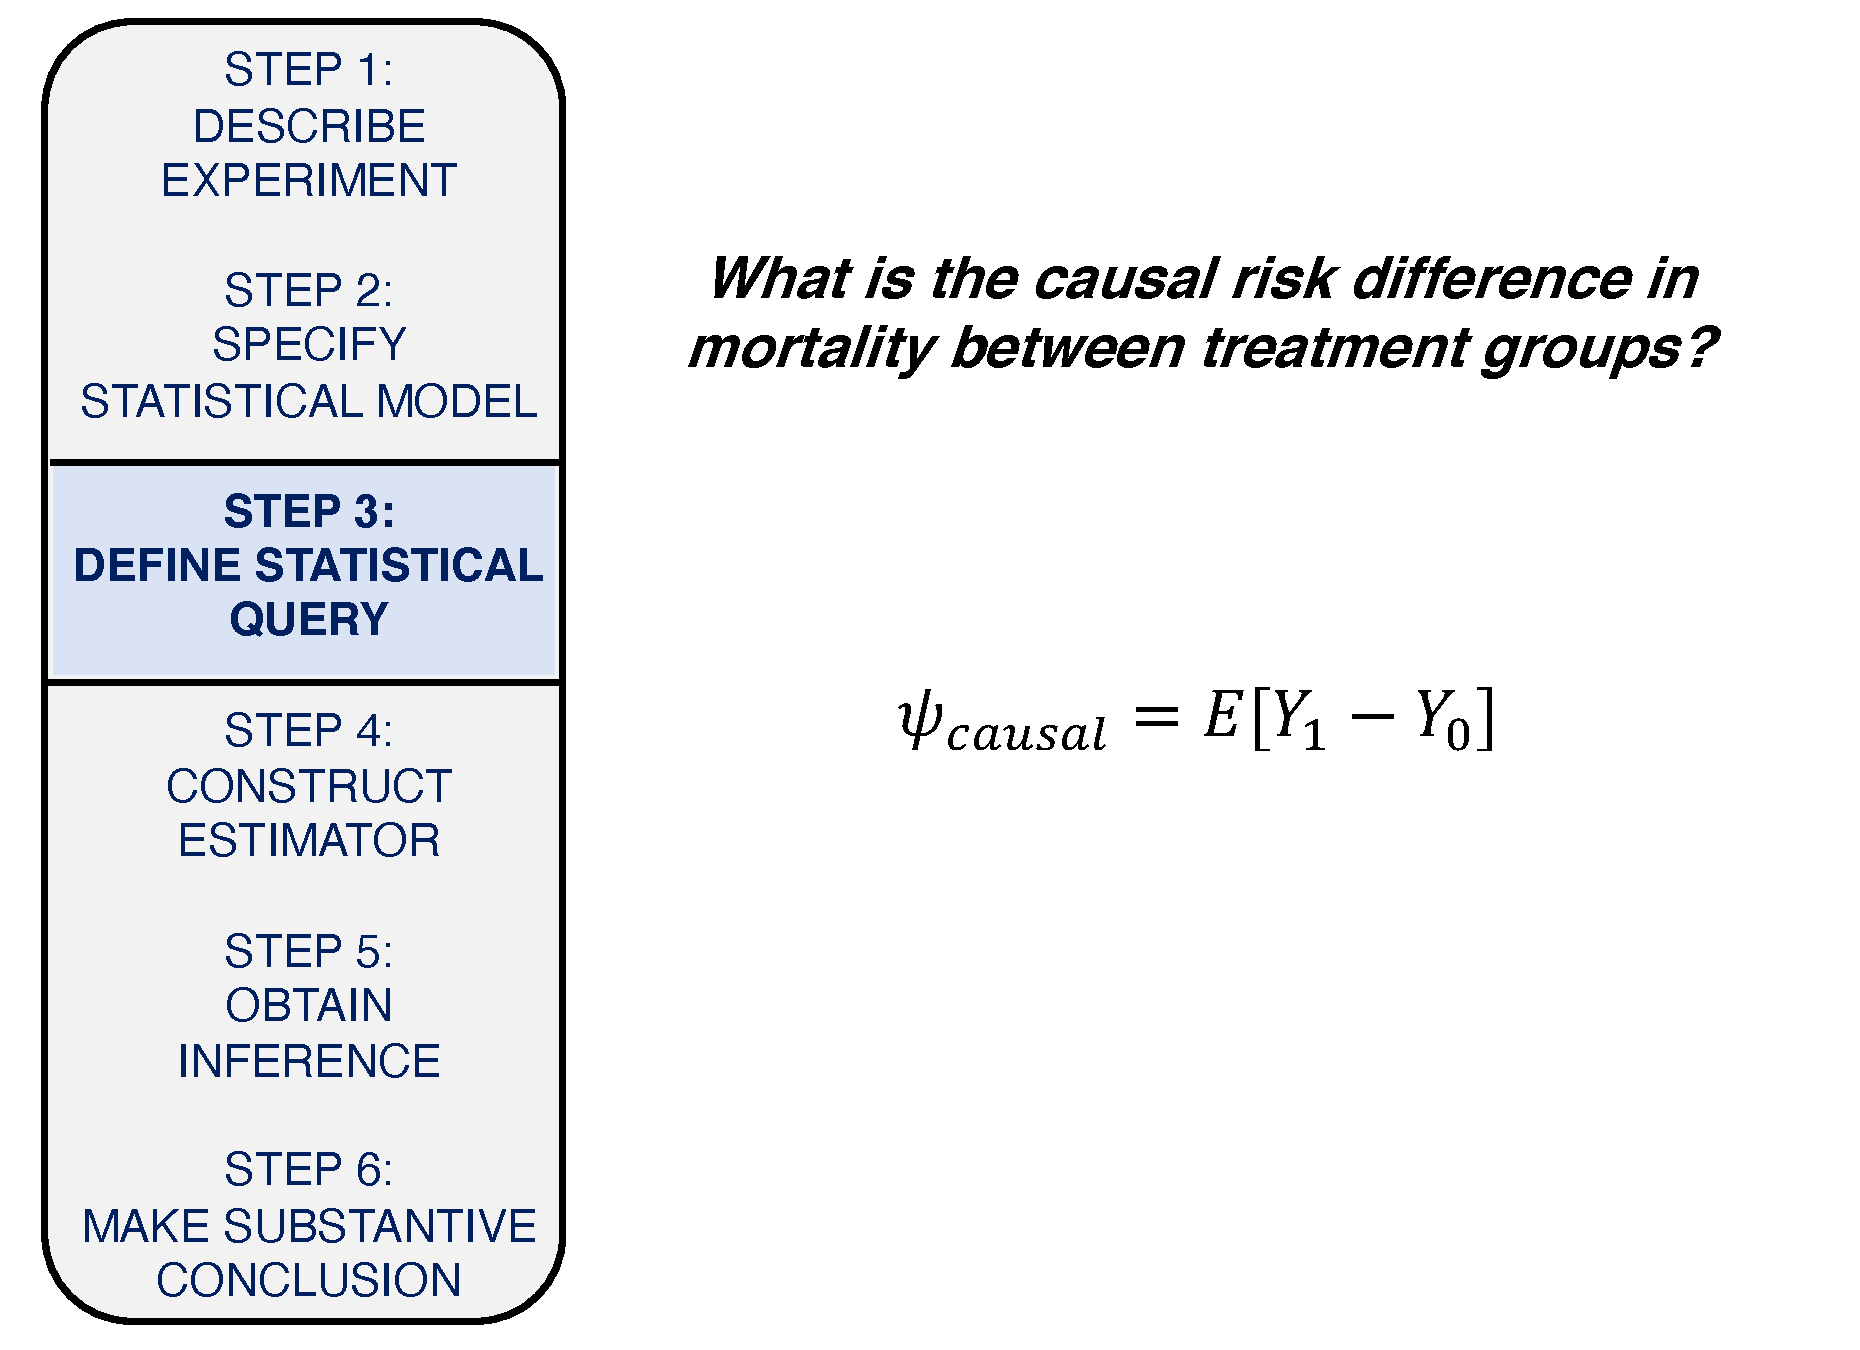
\includegraphics[width = 1.05\textwidth]{figures/roadmap3_1.pdf}
  \end{center}
\end{frame}

\begin{frame}
  \frametitle{Step 3b: What is the target statistical estimand that we will learn from the data?}
  \vspace{-20pt}
  \begin{center}
  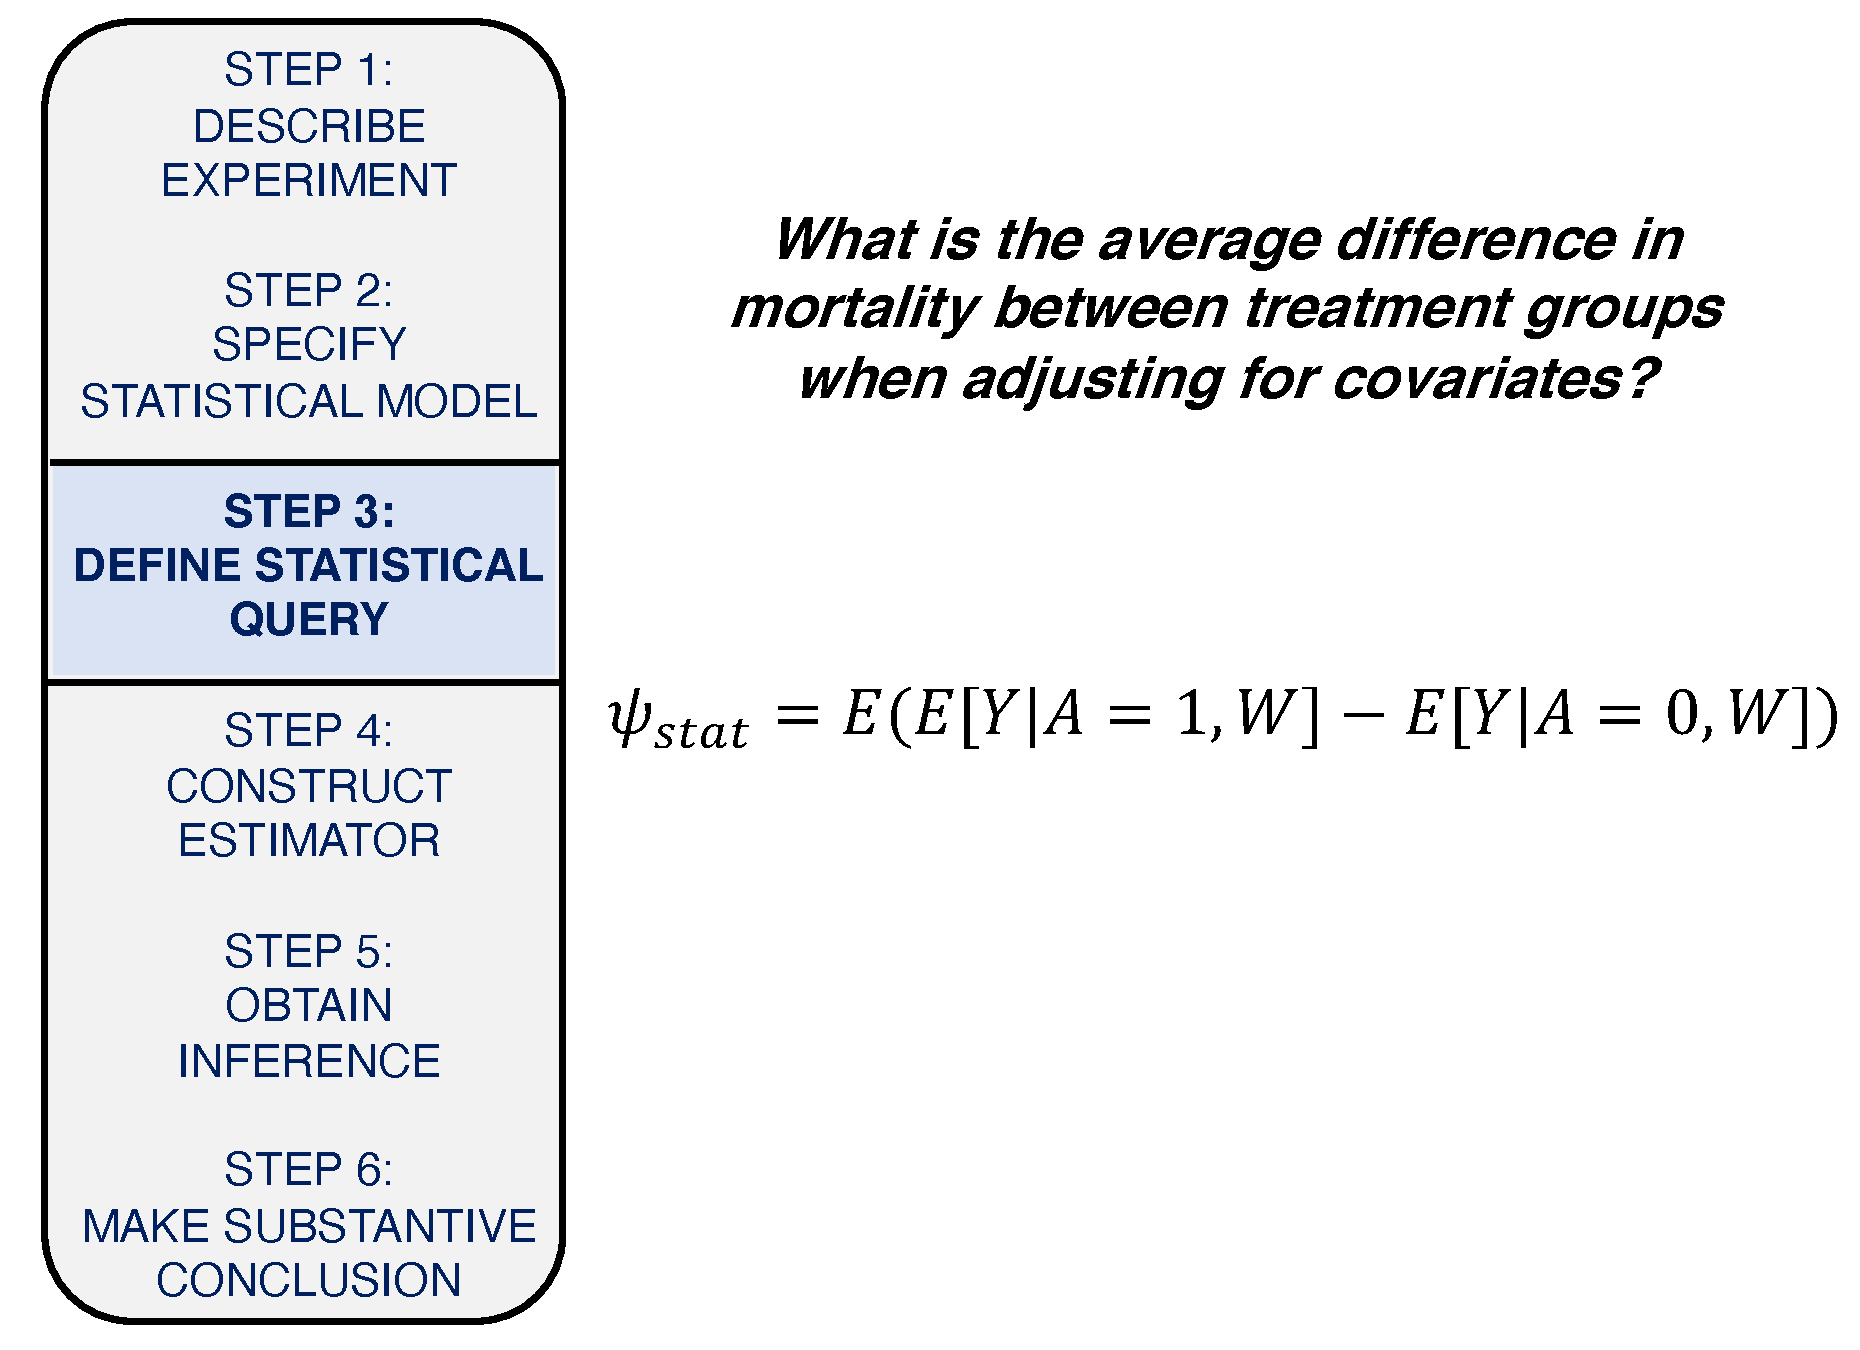
\includegraphics[width = 1.05\textwidth]{figures/roadmap3_2.pdf}
  \end{center}
\end{frame}

%\subsection{Construct estimator}
\begin{frame}
  \frametitle{How should we estimate the target estimand?}
  \vspace{-20pt}
  \begin{center}
  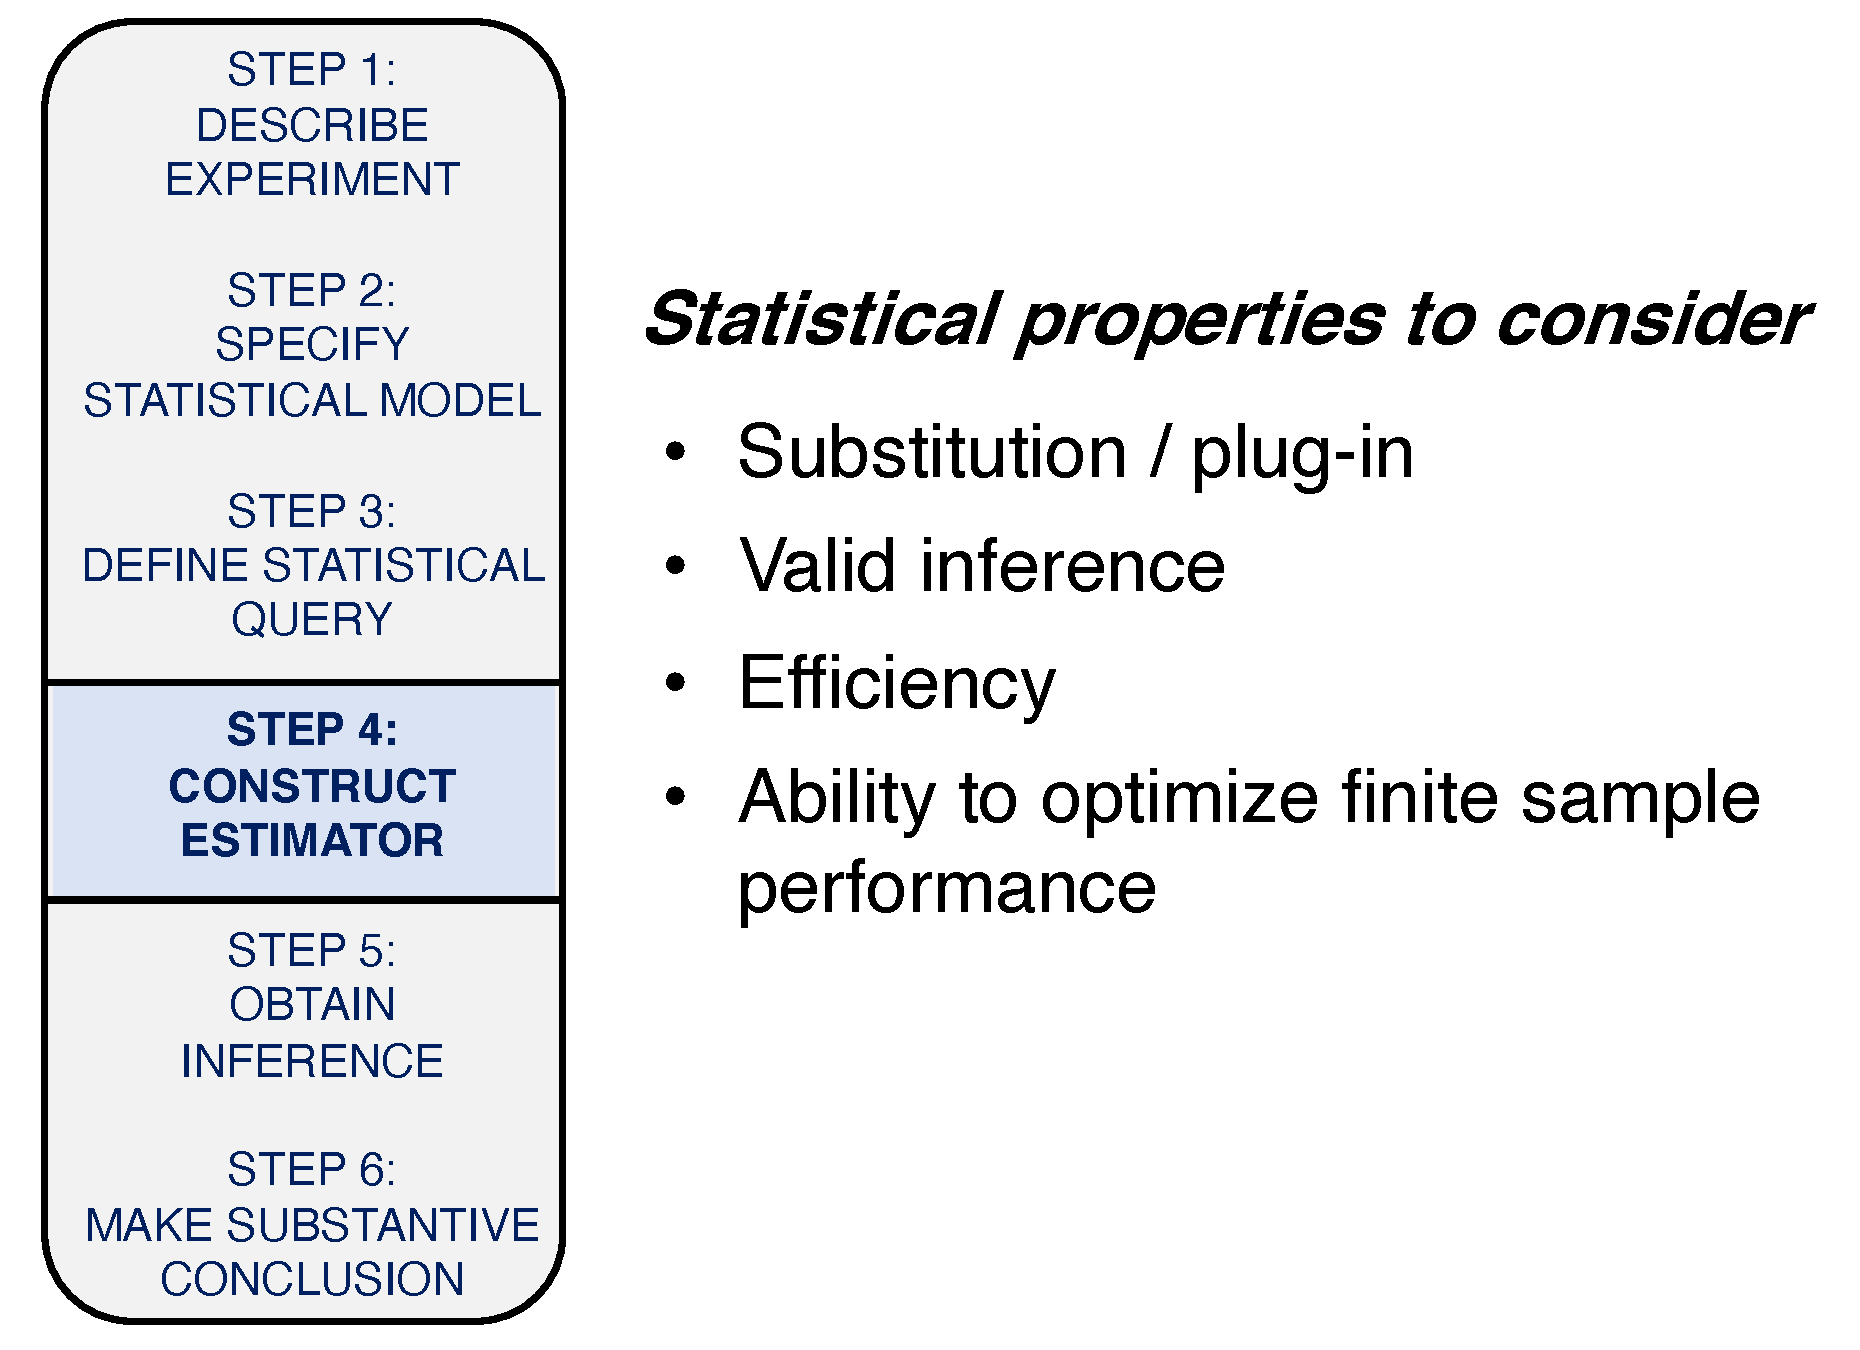
\includegraphics[width = 1.05\textwidth]{figures/roadmap4.pdf}
  \end{center}
\end{frame}

\begin{frame}
  \frametitle{Targeted Maximum Likelihood Estimation (TMLE)}
  \vspace{-20pt}
  \begin{center}
  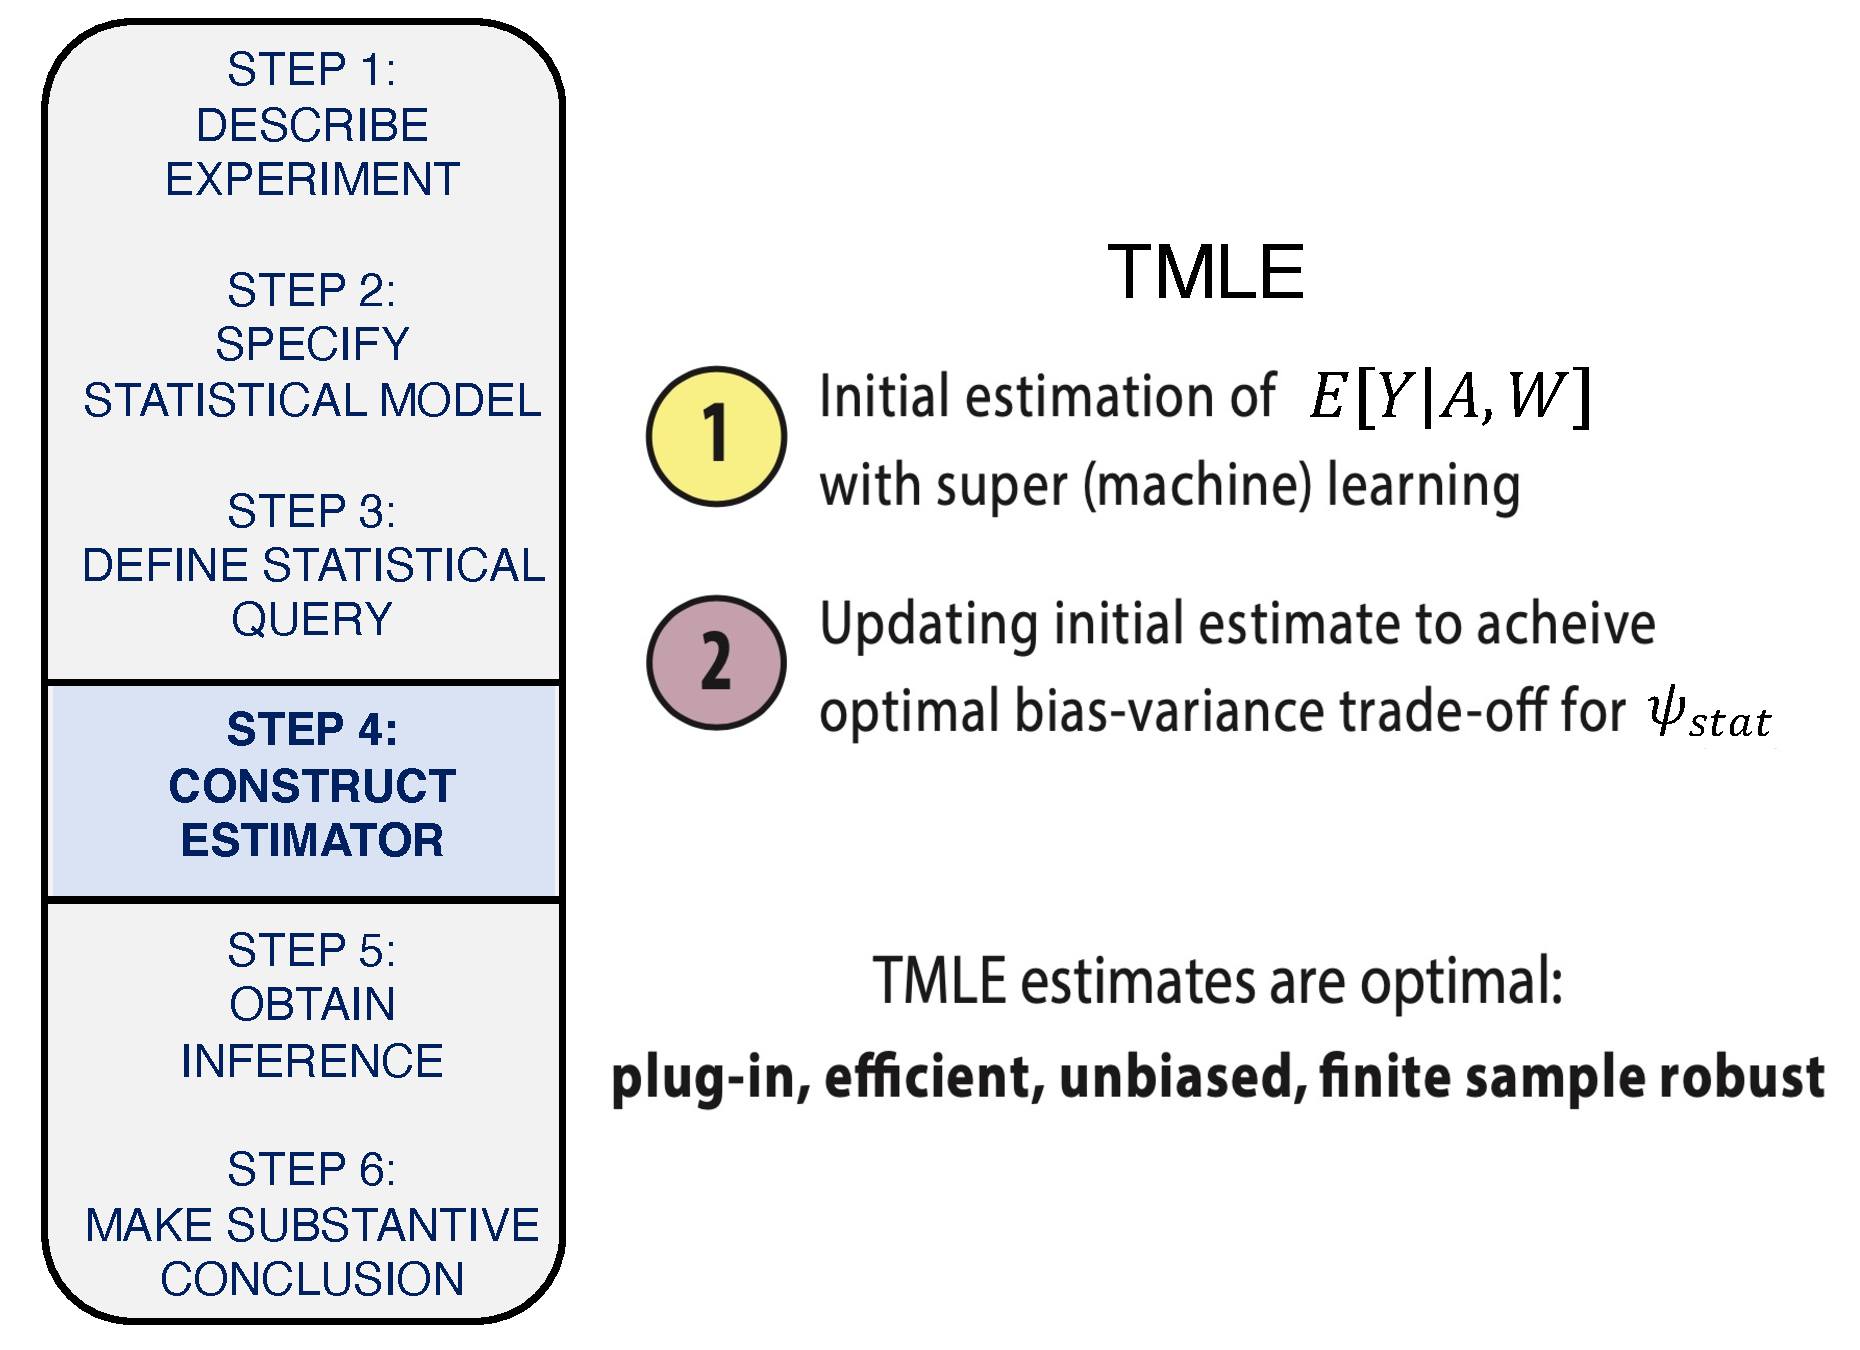
\includegraphics[width = 1.05\textwidth]{figures/roadmap4_1.pdf}
  \end{center}
\end{frame}
\begin{frame}
\frametitle{TMLE Step 1: Super learner}
\vspace{-15pt}
\begin{center}
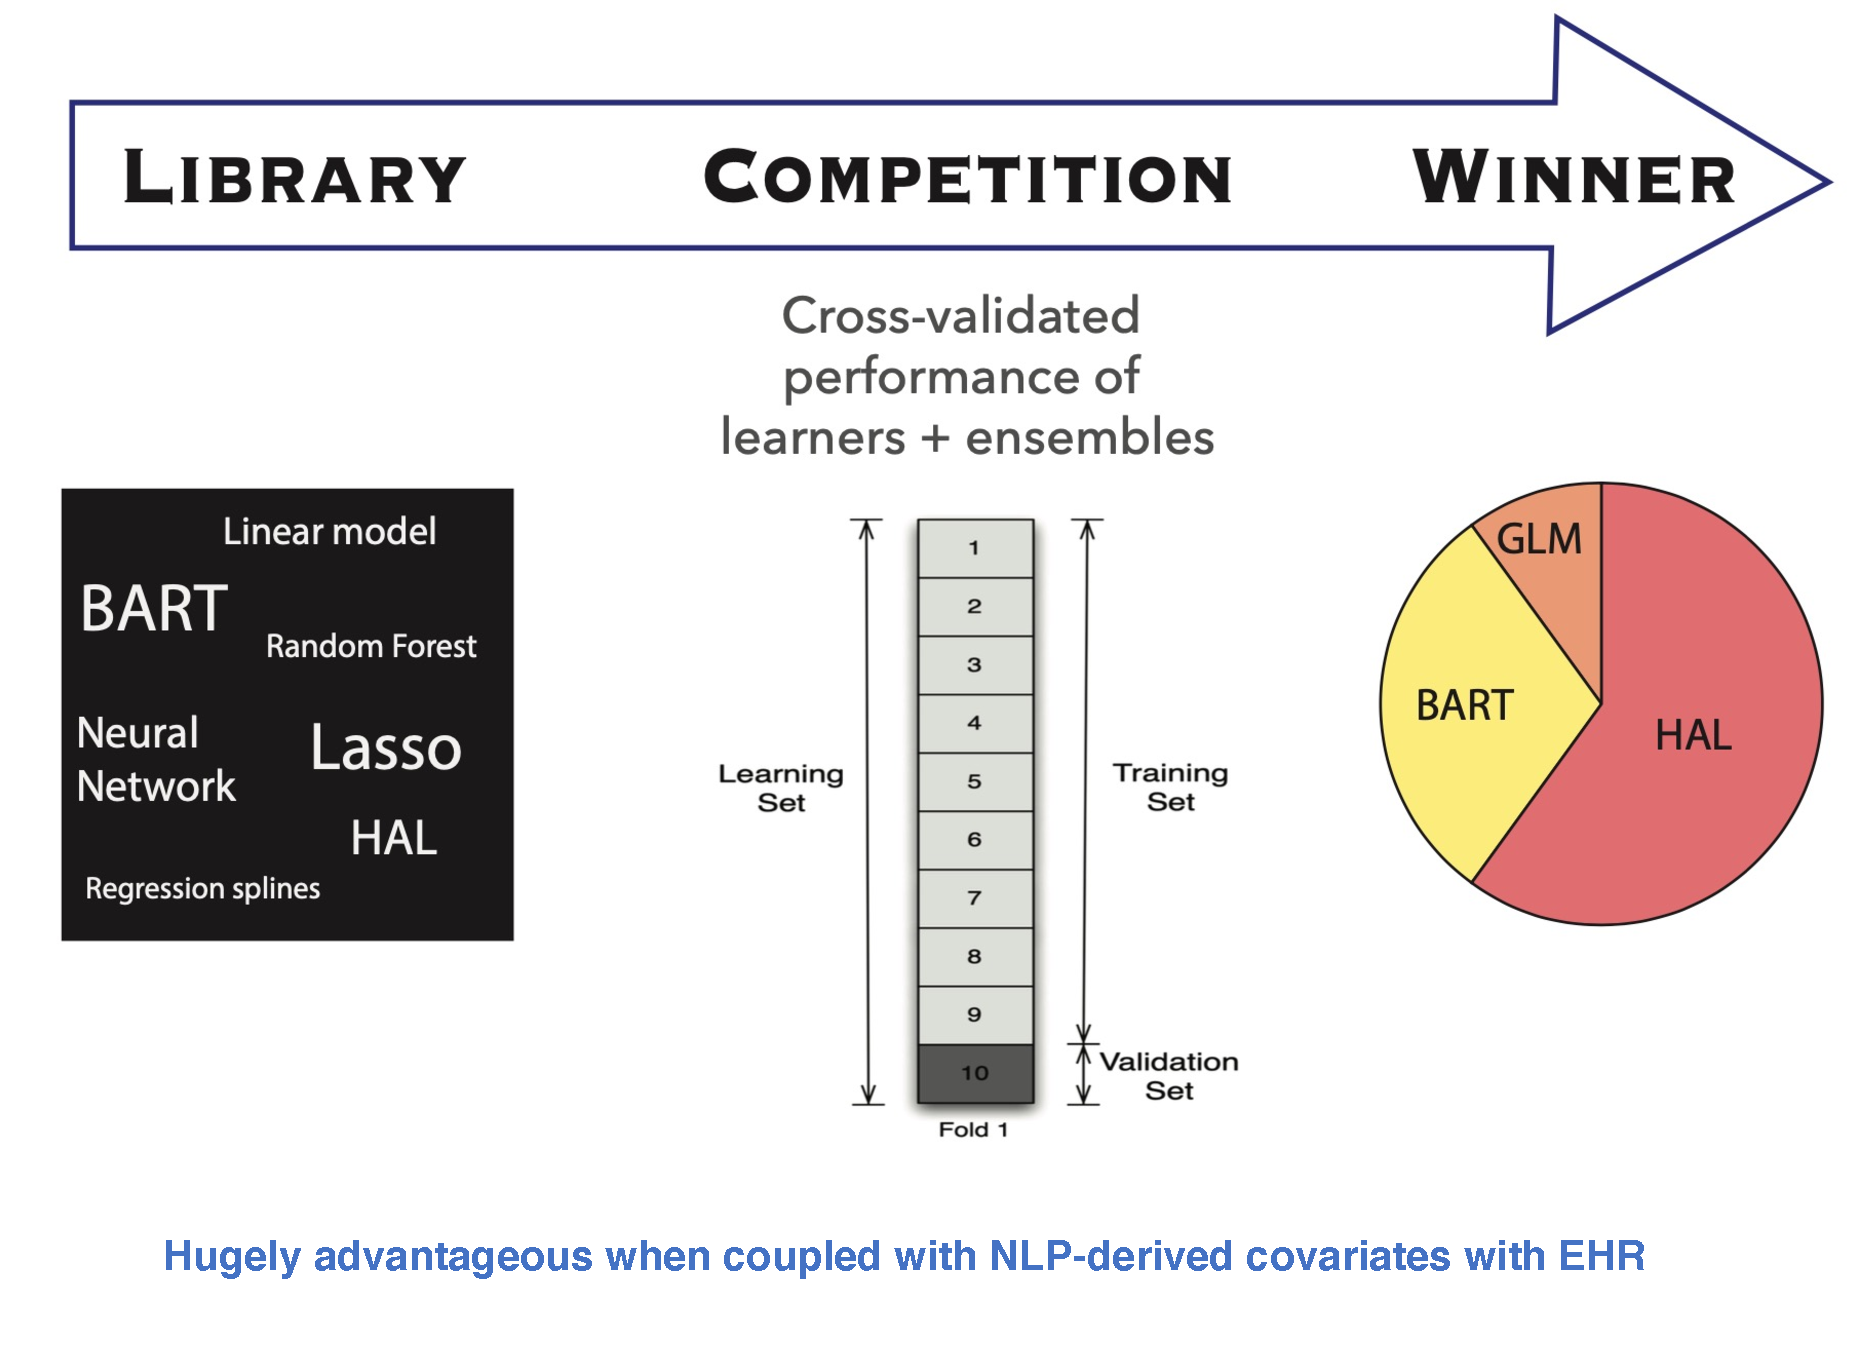
\includegraphics[width = 1\textwidth]{figures/SL.pdf}
\end{center}
\end{frame}

\begin{frame}
  \frametitle{Super learning across 15 data sets: Choice of algorithm adapts to data}
  \vspace{-.5in}
  \begin{figure}
  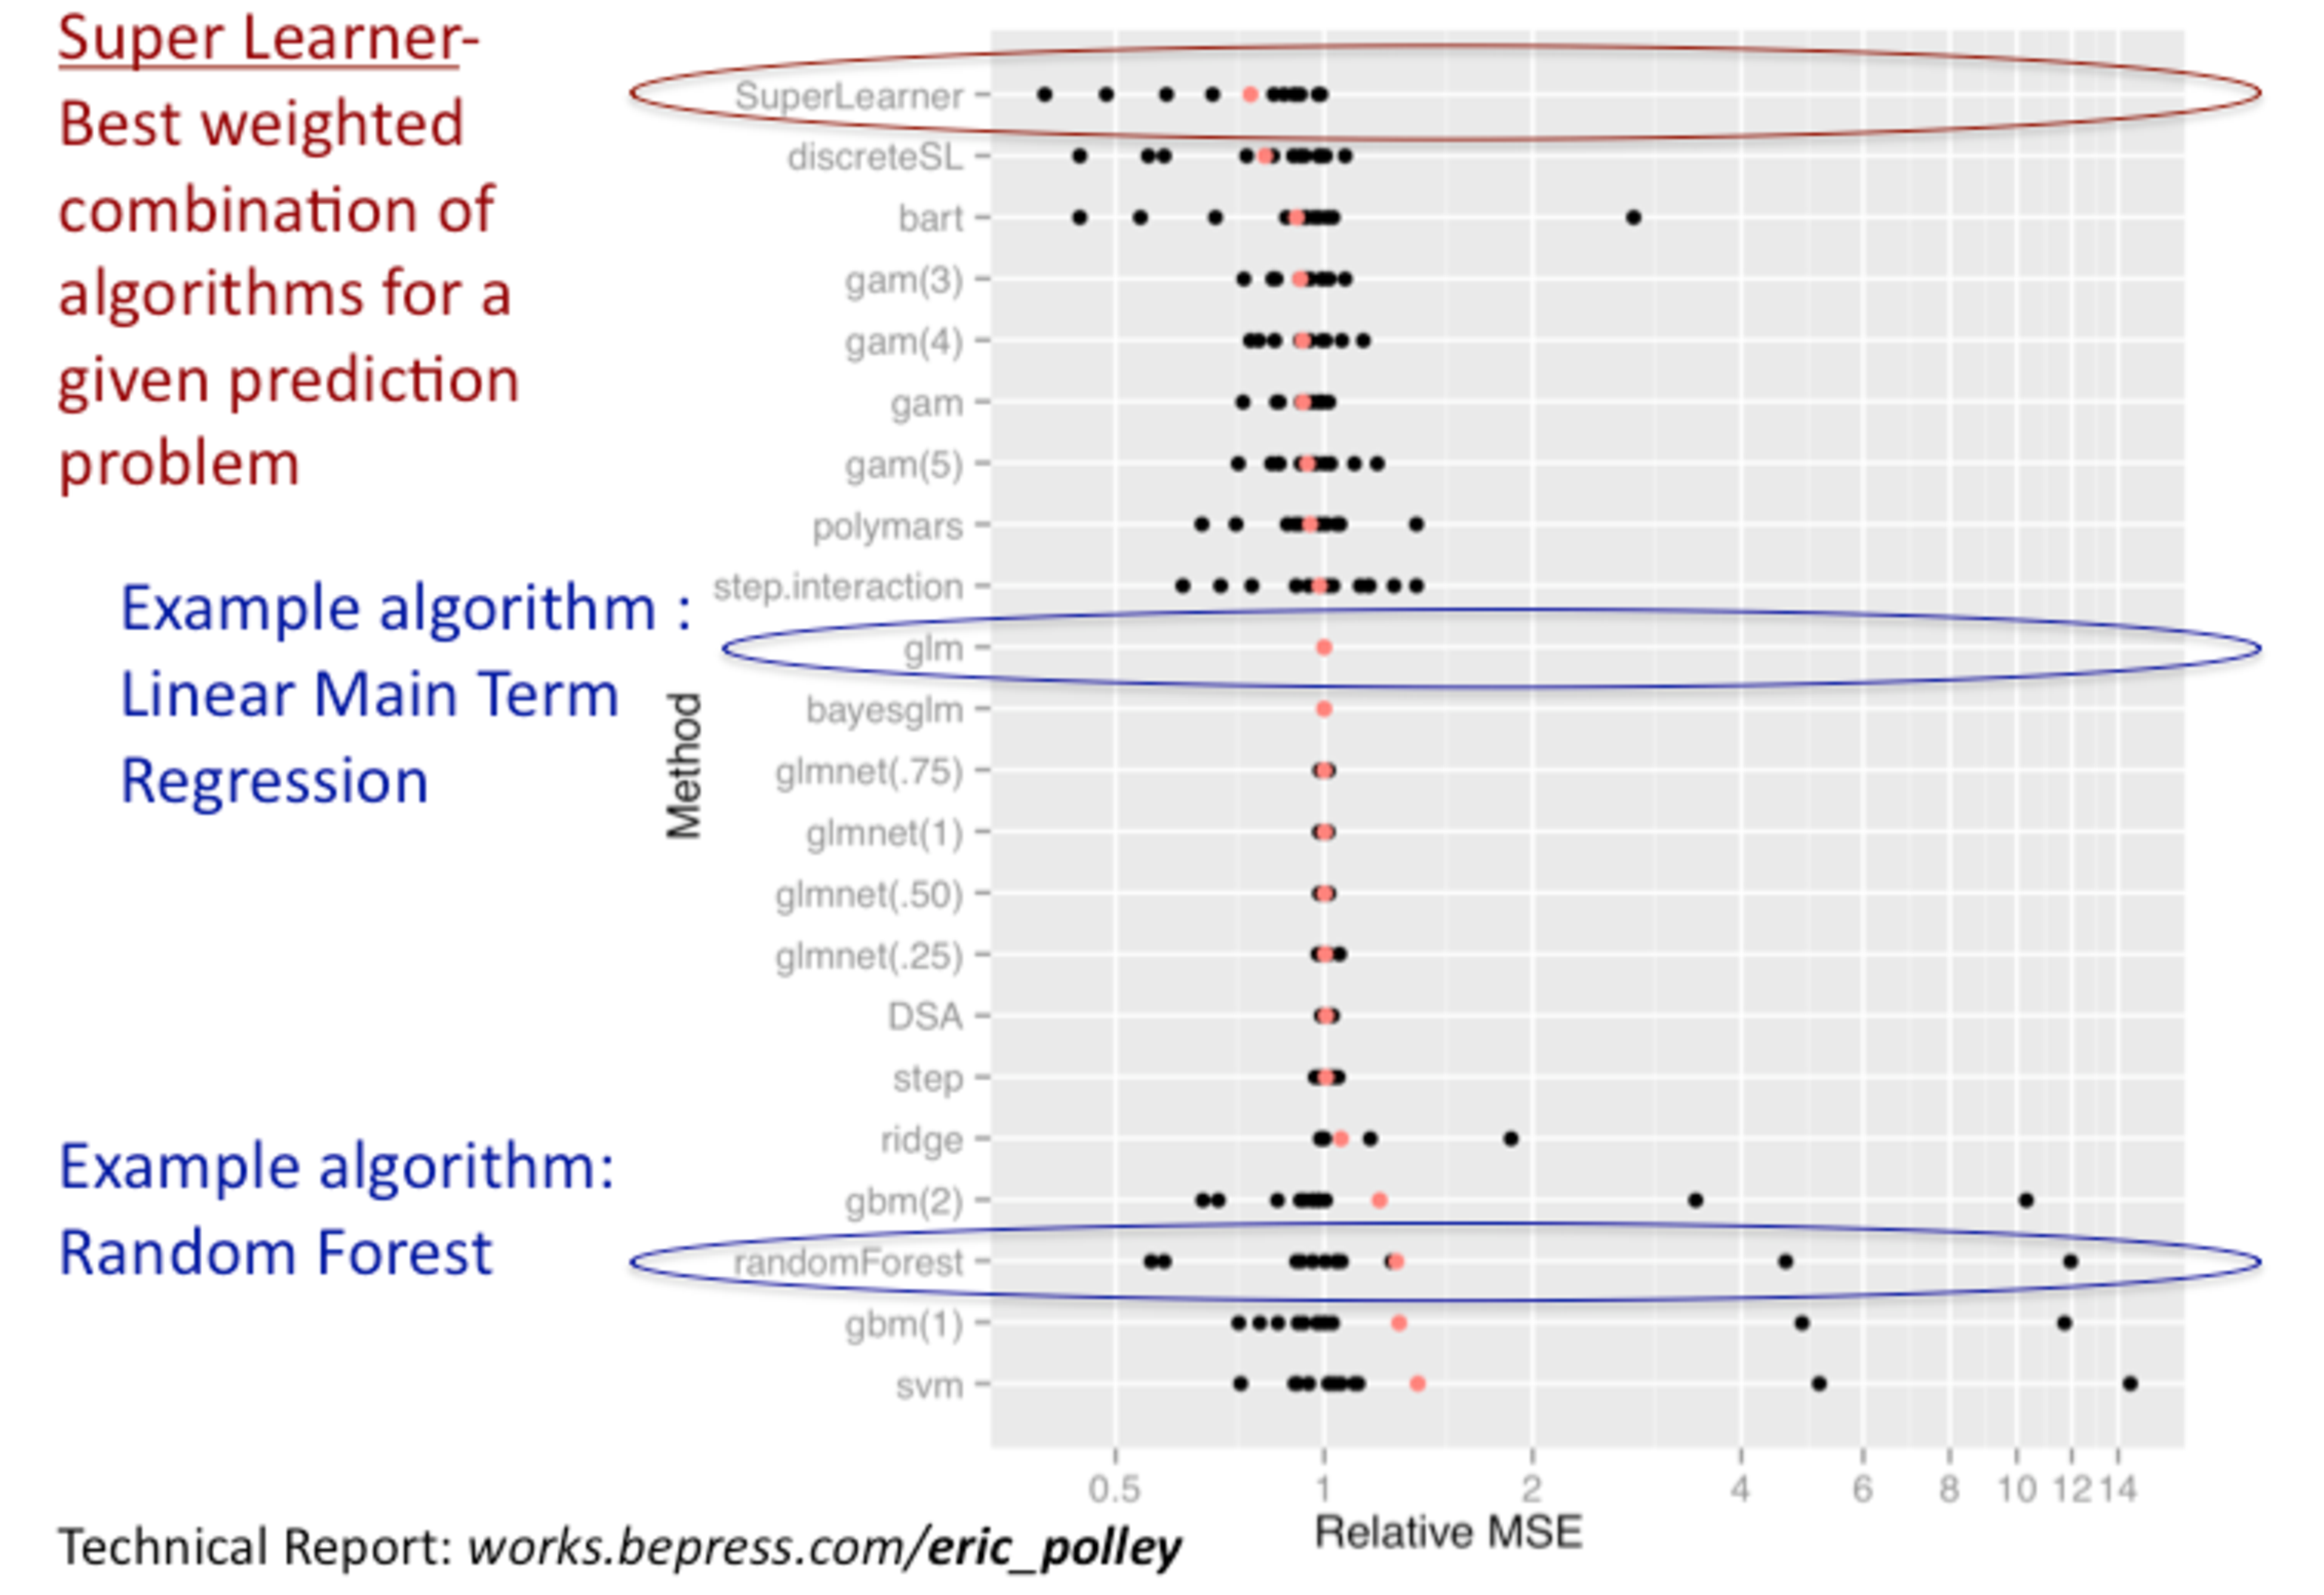
\includegraphics[width=1.1\textwidth]{ericSL}
  \end{figure}
\end{frame}

\begin{frame}
%  \frametitle{Super learning: data demonstration}
  \vspace{-.1in}
  \begin{figure}
  \includegraphics[width=1.0\textwidth]{mayaslides/Slide35.png}
  \end{figure}
\end{frame}
%\frametitle{Highly Adaptive Lasso (HAL)}\begin{block}{\large{Key Idea}}\begin{itemize}\vspace{.1in}\item Any $d$-dimensional cadlag function (i.e.~right-continuous) can be represented as a possibly infinite linear combination of spline basis functions.\vspace{.05in}\item The variation norm / complexity of a function is the $L_1$-norm of the vector of coefficients.\vspace{.1in}\end{itemize}\end{block}\vspace{.25in}\begin{center}{\large Converges to true function at rate $n^{-1/3}(\log n)^{d/2}$}\end{center}\end{frame}

%\begin{frame}\frametitle{HAL performance for d=3}  \vspace{-10pt}  \begin{center}  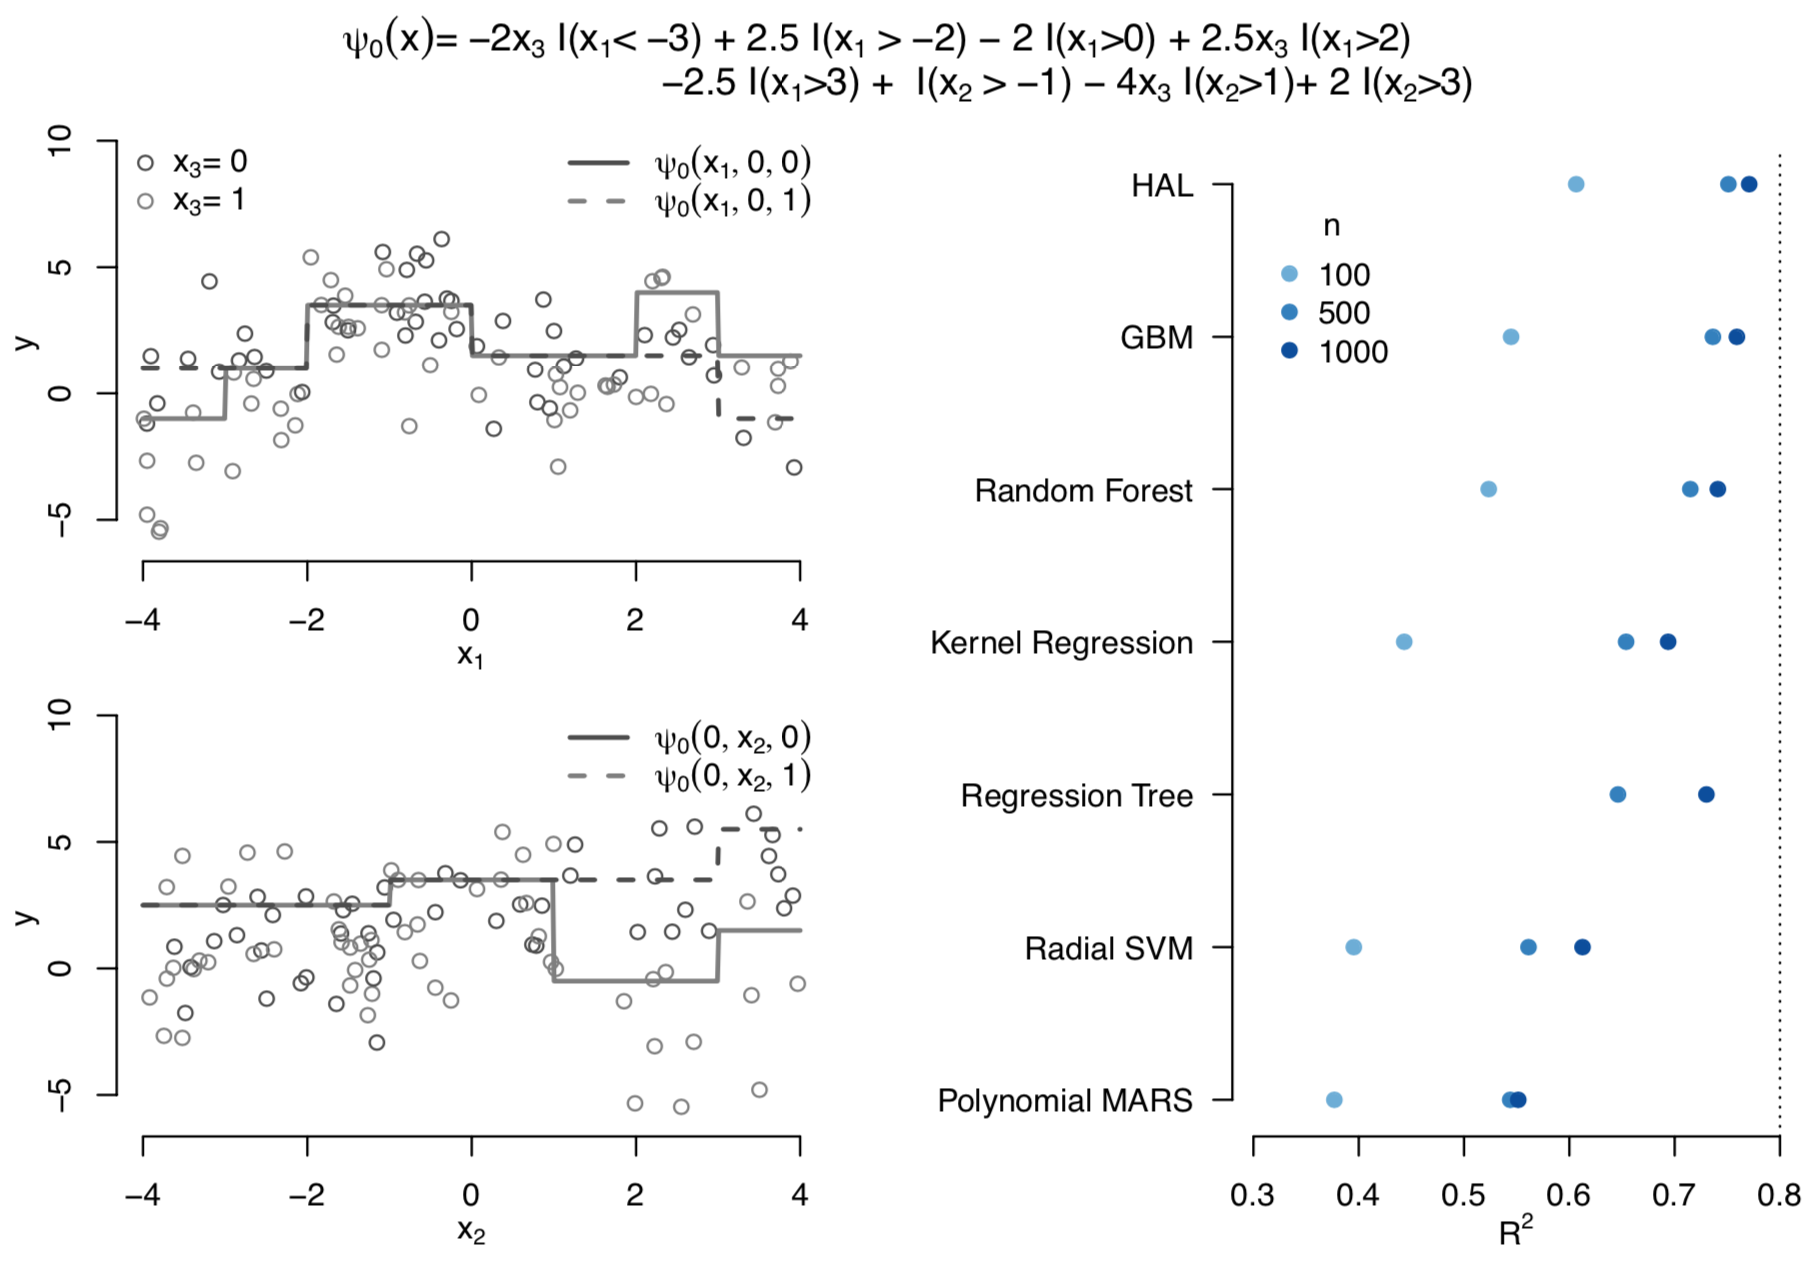
\includegraphics[width = 1\textwidth]{HALworks.png}  \end{center}\end{frame}

%\begin{frame}{New Results: Asymptotic normality of higher order HAL itself, van der Laan, 2023}\begin{itemize}\item Defined higher order smoothness classes $D^{(k)}([0,1]^d)$.\item $D^{(k)}([0,1]^d)$ can be represented as linear span of tensor products of $\leq k$-th order spline basis functions.\item With $O(J)$ basis function, we obtain uniform approximation error $O(1/J^{k^*})$ up till $\log J$-factor, $k^*=k+1$. \item HAL-MLE $Q_n=\sum_{j\in {\cal R}_n}\beta_n(j)\phi_j$ with $J_n$  non-zero coefficients of its oracle MLE  $Q_{0,n}=\sum_{j\in {\cal R}_n}\beta_{0,n}(j)\phi_j$ satisfies $(J_n/n)^{1/2}(Q_n-Q_{0,n})(x)\Rightarrow_d N(0,\sigma^2_0(x))$, while $|| Q_{0,n}-Q_0 ||_{\infty}\sim O(1/J_n^{k^*})$. \item By selecting $J_n\sim n^{-1/(k^*+1)}$, rate equals $n^{-k^*/(2k^*+1)}$ up till $\log n$-factors.\item At cost of another $\log n$-factor this rate is uniform in $x$. \item Pointwise and uniform confidence intervals follow.\end{itemize}\end{frame}

%\begin{frame}\frametitle{TMLE Step 2: Targeting follows a path of maximal change in target estimand per unit likelihood}\vspace{-12pt}\centering\begin{figure}\centering\animategraphics[autoplay,loop,width=0.95\linewidth]{7}{ULFS_n400/gganim_plot}{0001}{0100}\end{figure}\end{frame}


%\subsection{Obtain inference}\begin{frame}  \frametitle{How should we approximate the sampling distribution of our estimator?}  \vspace{-20pt}  \begin{center}  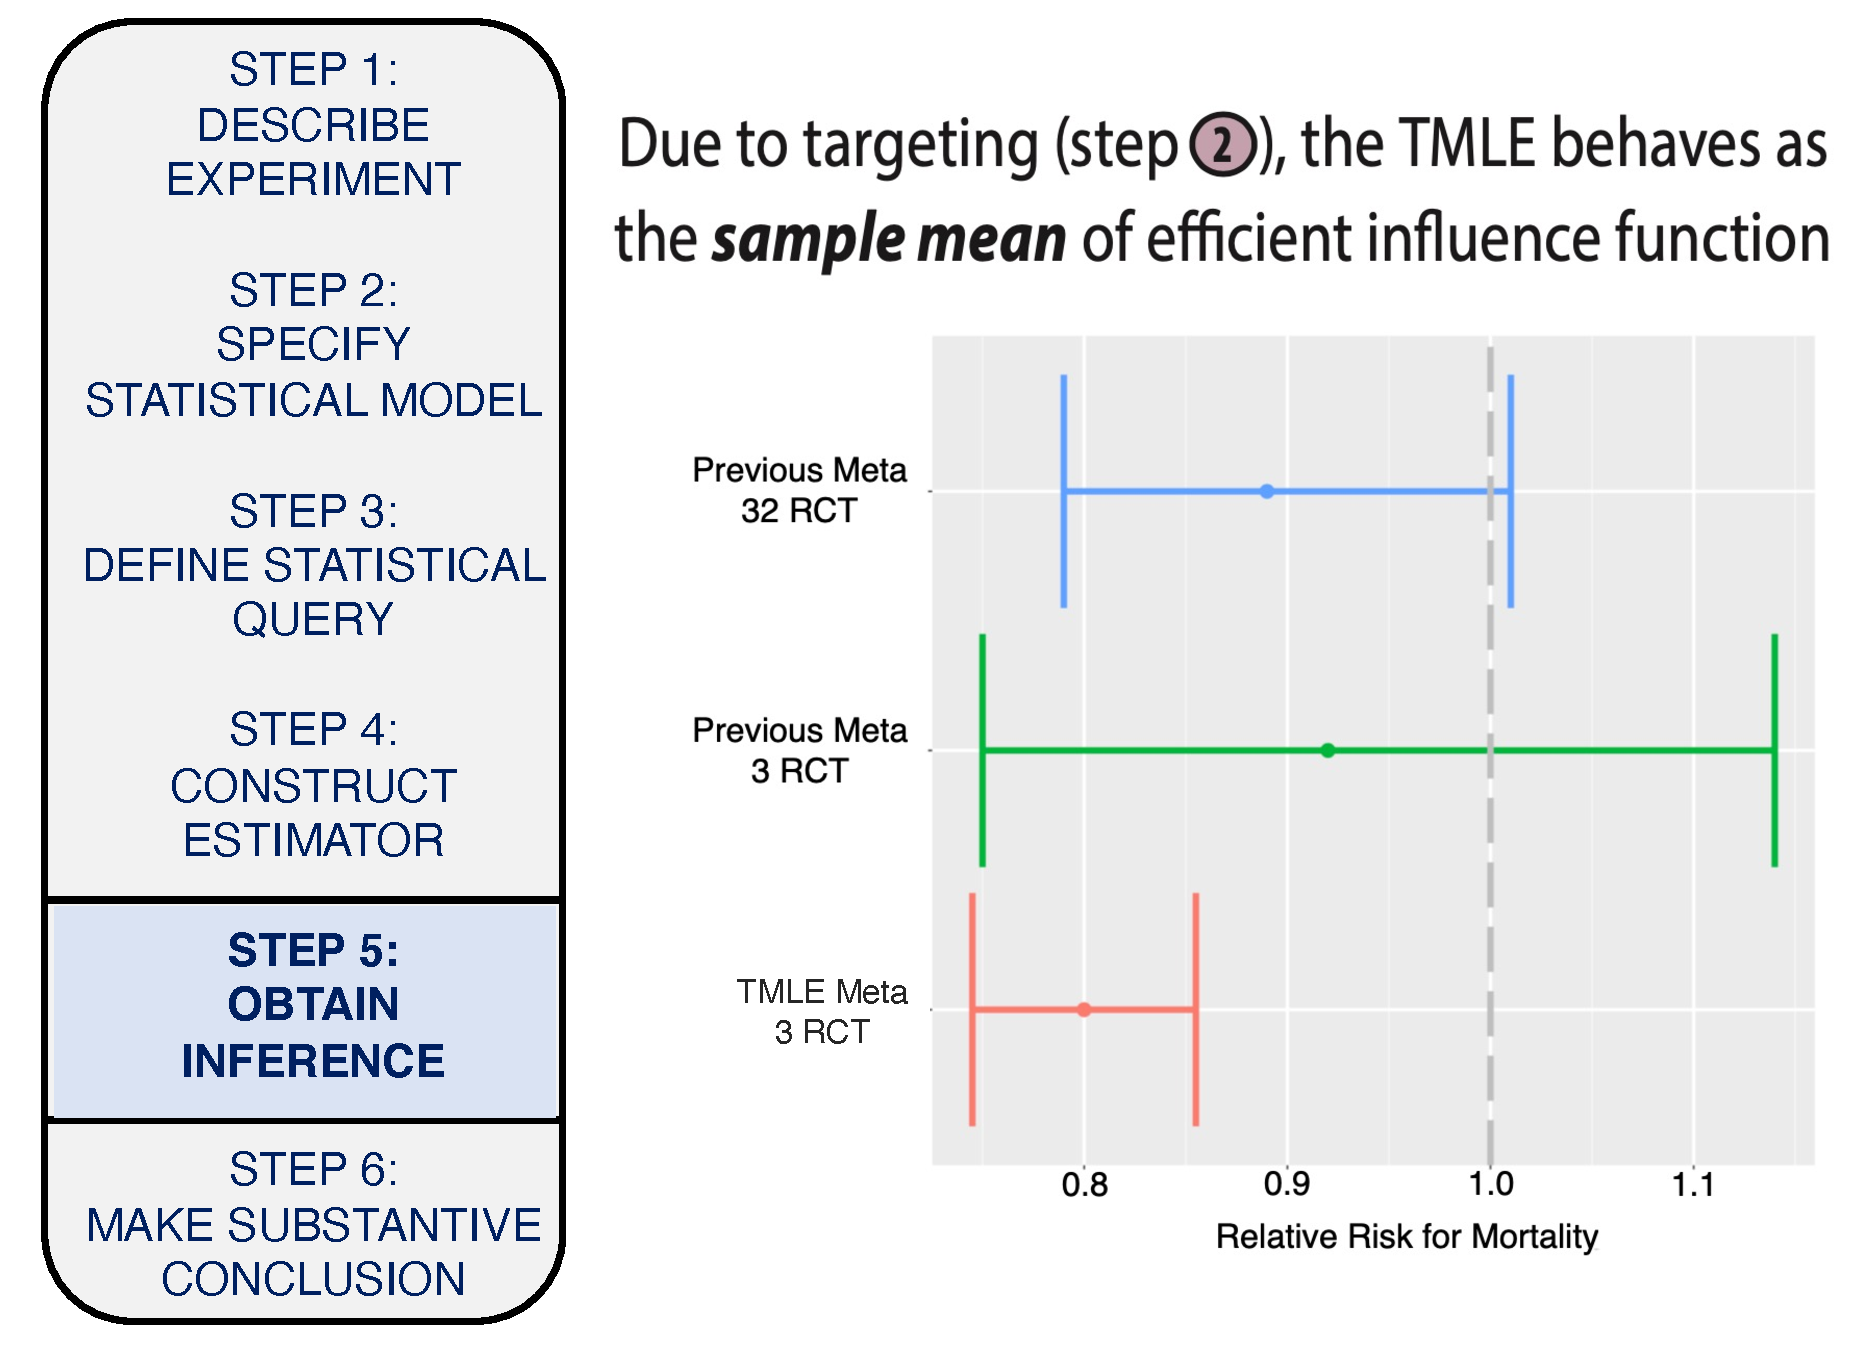
\includegraphics[width = 1.05\textwidth]{figures/roadmap5.pdf}  \end{center}\end{frame}

%\begin{frame}\frametitle{Can we break HAL-TMLE?}\vspace{-15pt}\begin{center}\includegraphics[width = 1\textwidth]{coverageByN.pdf}\end{center}\end{frame}


%\begin{frame} \frametitle{Possibility to refine question of interest and inform future studies}  \vspace{-11pt}  \begin{center}  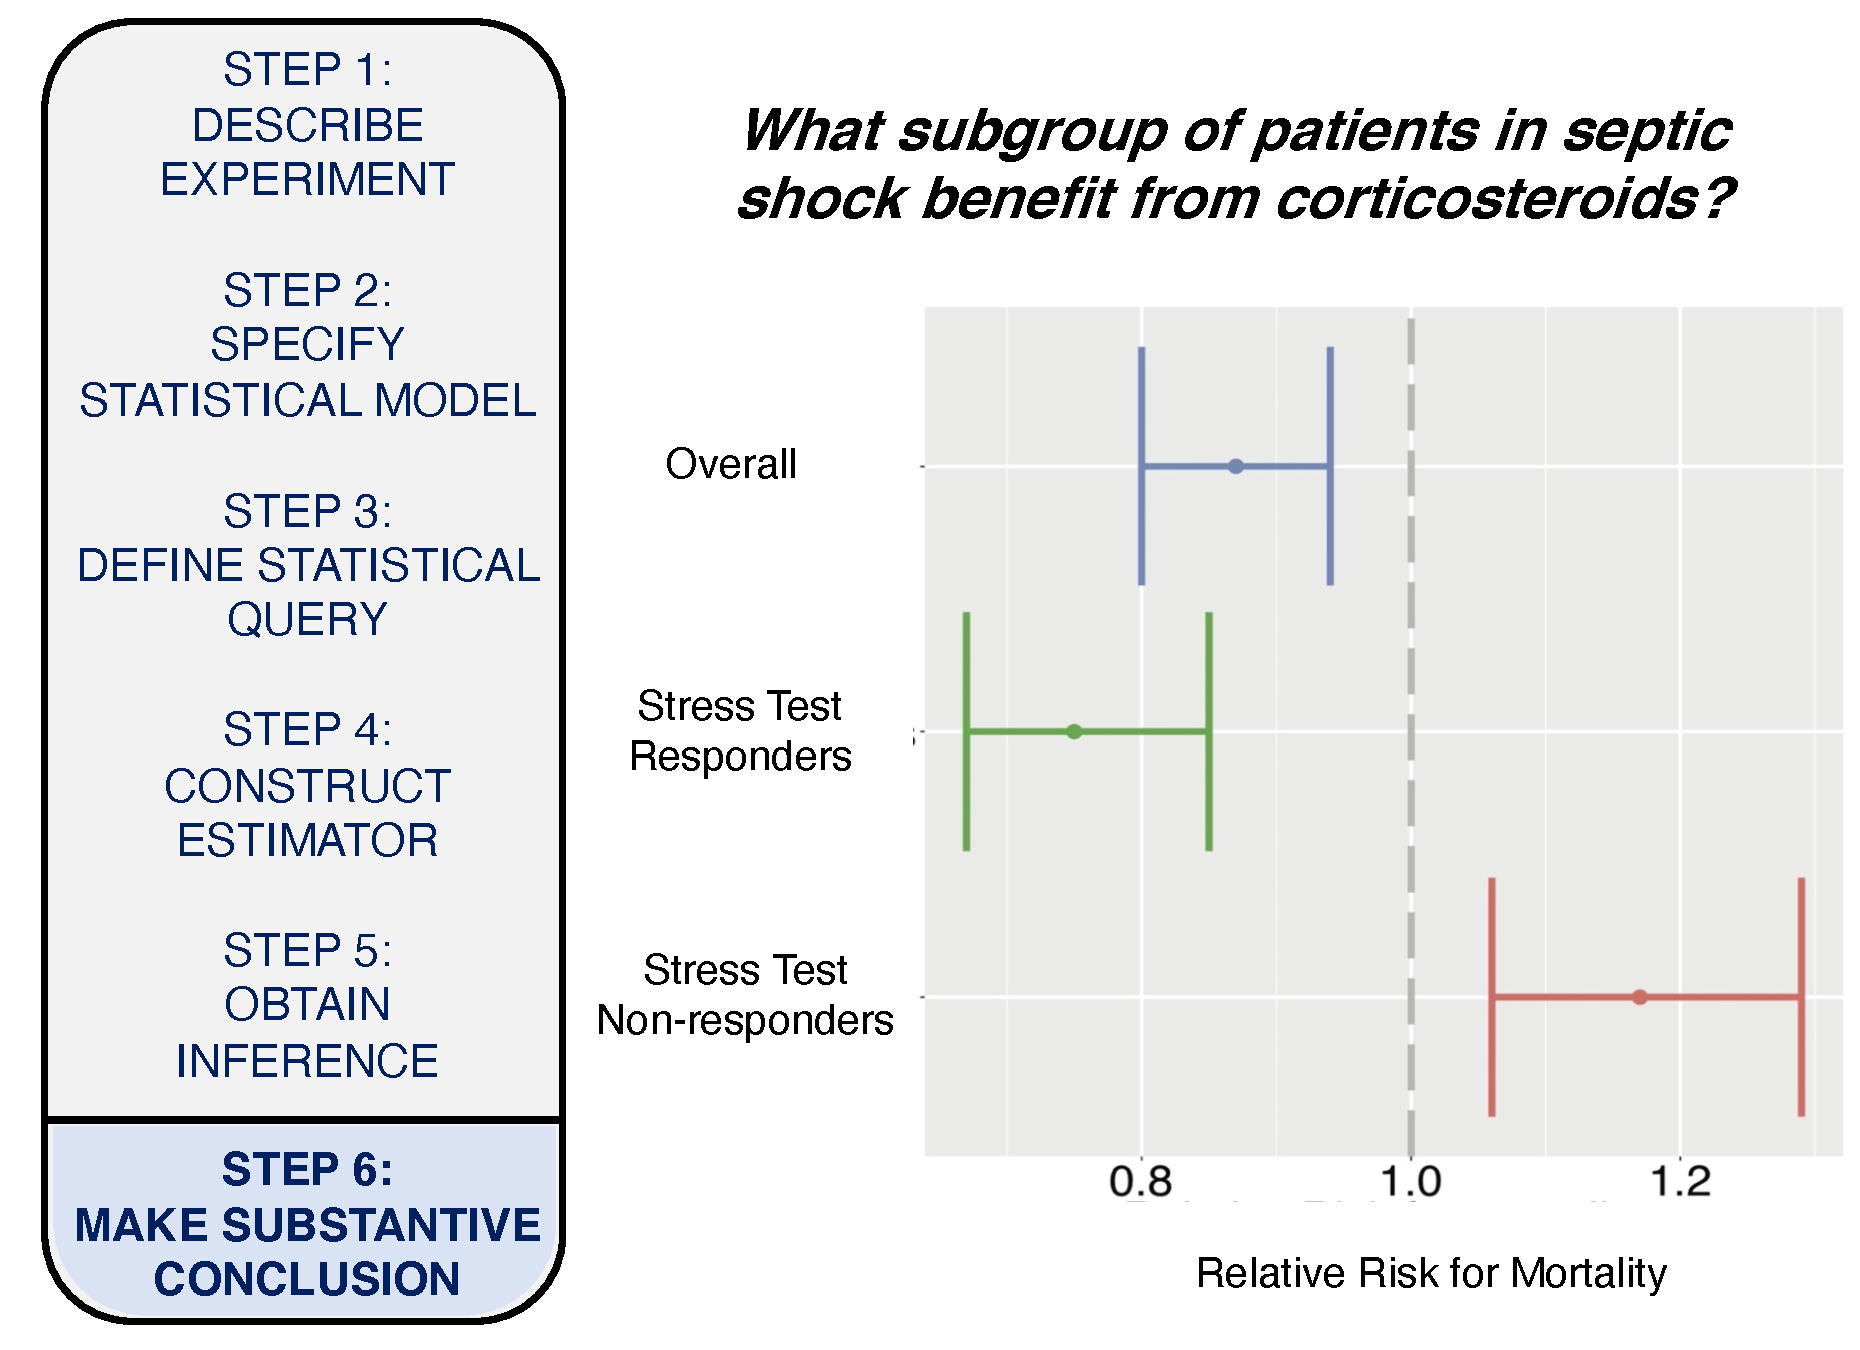
\includegraphics[width = 1.0\textwidth]{figures/roadmap_alt1.pdf}  \end{center}\end{frame}

%\subsection{Make substantive conclusion}

\begin{frame}
\frametitle{Arriving at the substantive conclusion}
\vspace{-16pt}
  \begin{center}
  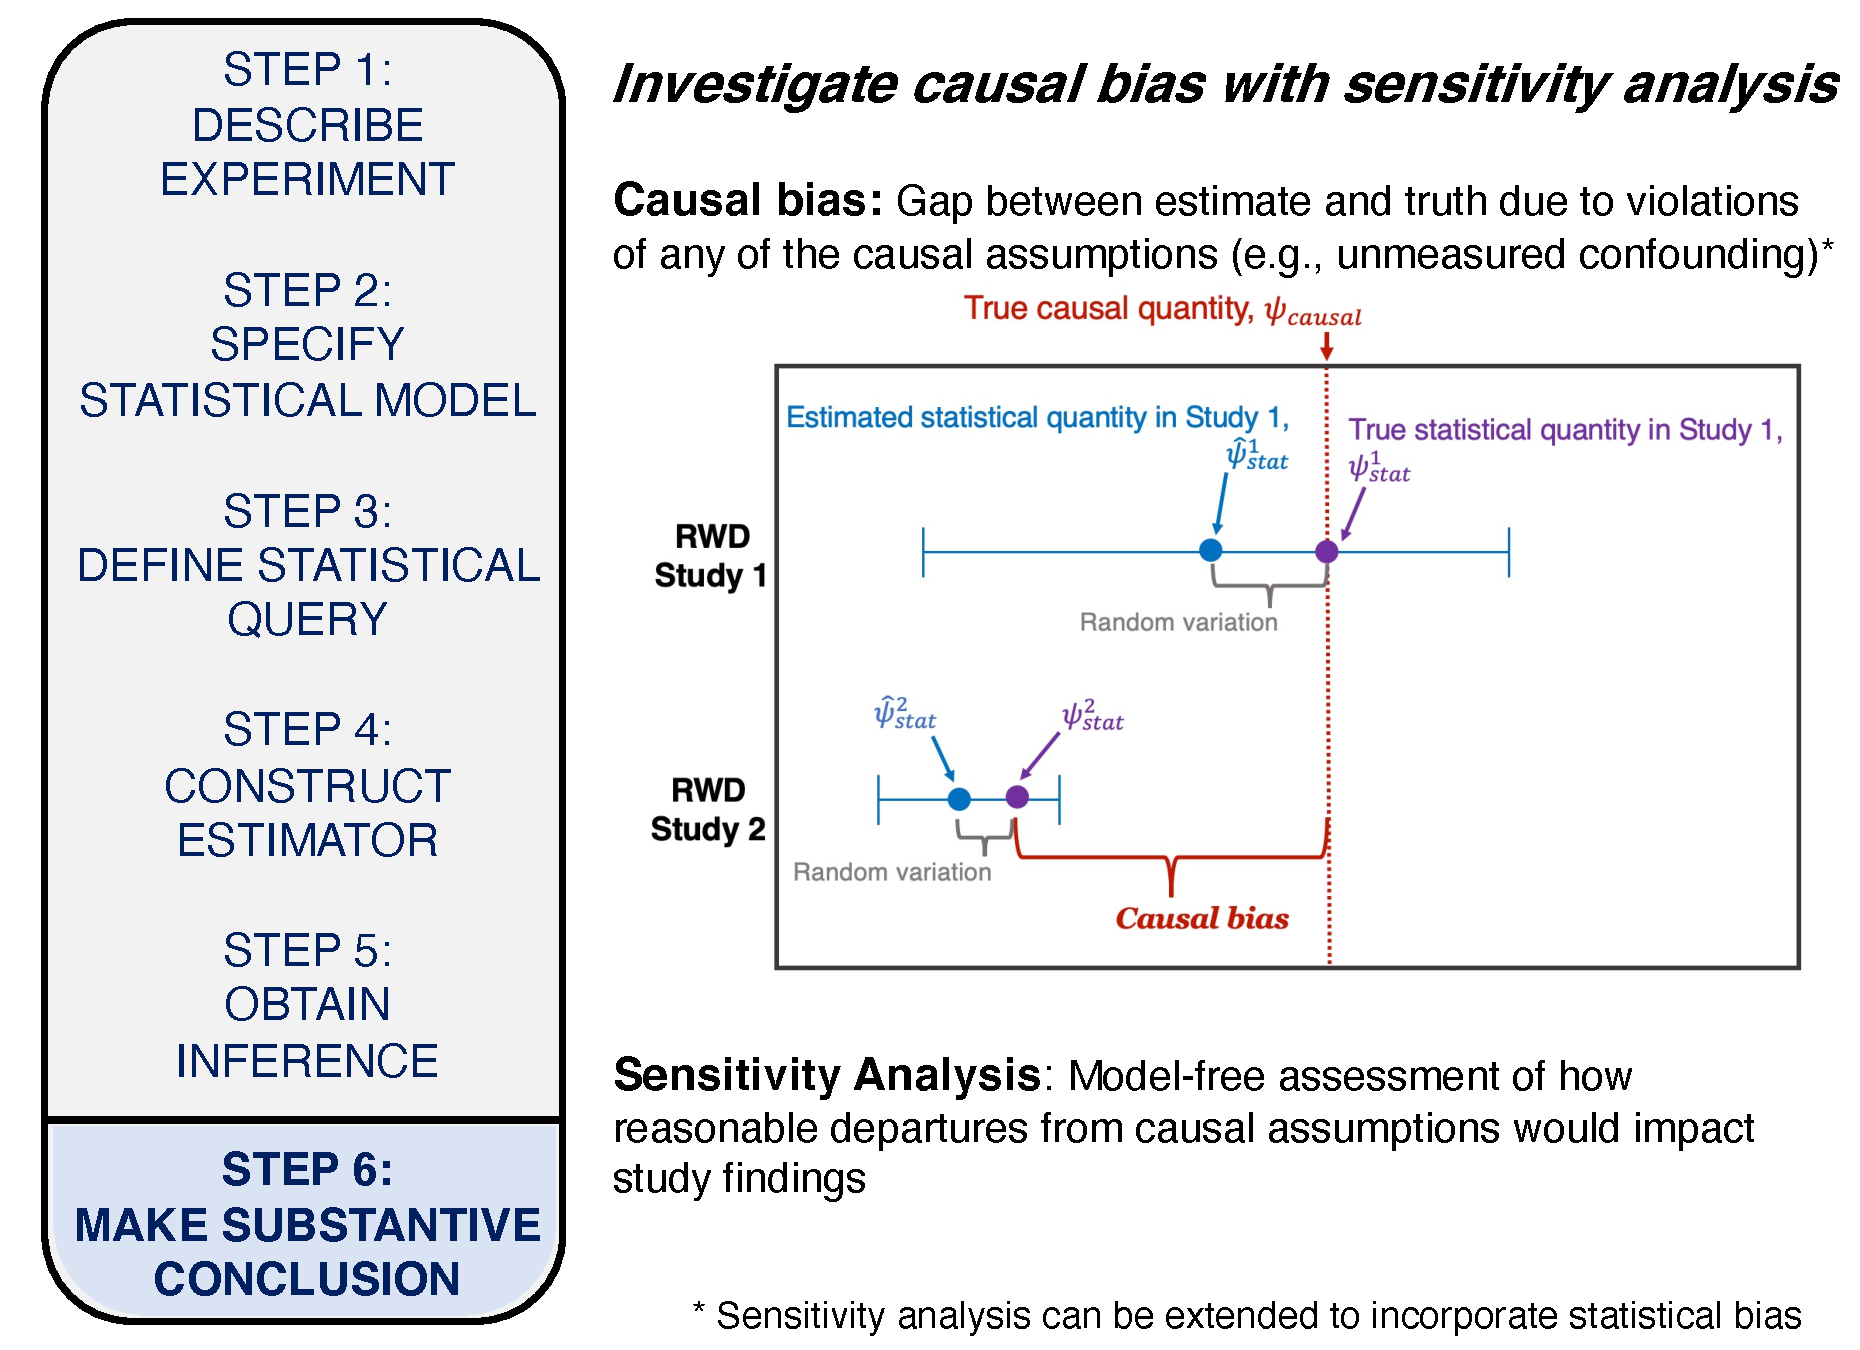
\includegraphics[width = 1.02\textwidth]{figures/roadmap6.pdf}
  \end{center}
%  \small{Could use negative controls to obtain further insight in plausible causal gap}
\end{frame}

\begin{frame}
\frametitle{TL-based non-parametric sensitivity analysis
RCT with 25\% LTFU example}
\vspace{-10pt}
  \begin{center}
  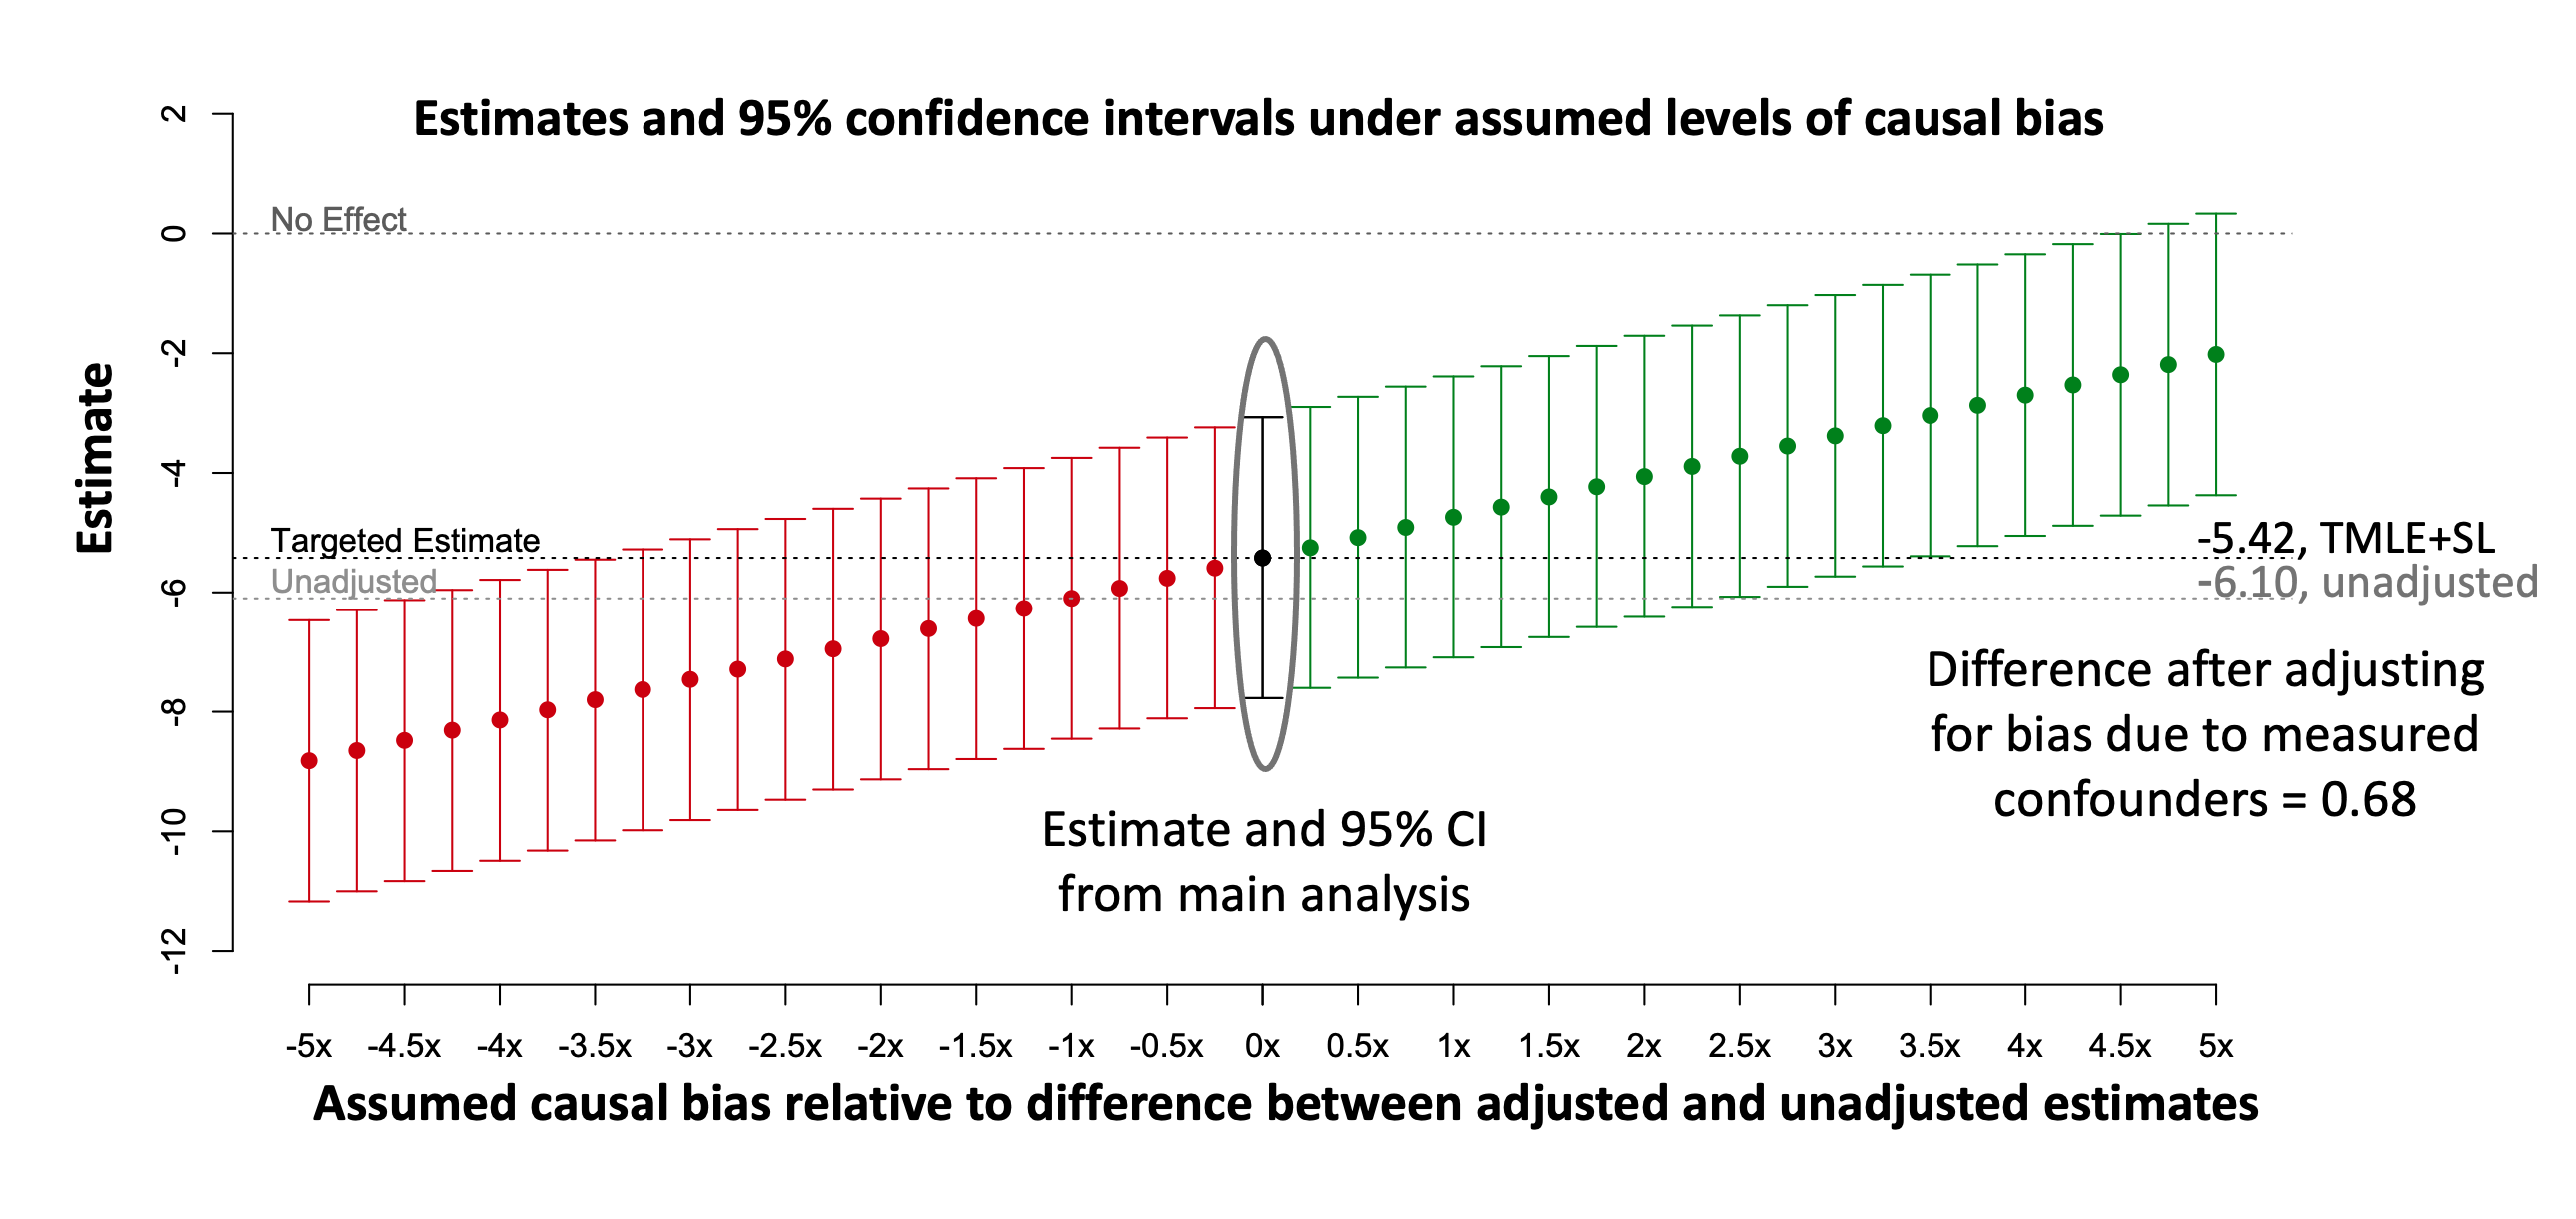
\includegraphics[width = 1.05\textwidth]{figures/gruber_sensitivity.png}
  \end{center}
   \small{Could use negative controls to obtain further insight in plausible causal gap}\ \newline\newline\newline\newline 
  \vspace{35pt}
\tiny{Courtesy of "Targeted-Learning Based Statistical Analysis Plan" Webinar by Susan Gruber on 28 April 2021}
%\tiny{Can bring in negative controls for further insight in plausible causal gap}
\end{frame}

\begin{frame}
\frametitle{TL-based non-parametric sensitivity analysis:

Safety analysis example}

\vspace{-18pt}
  \begin{center}
  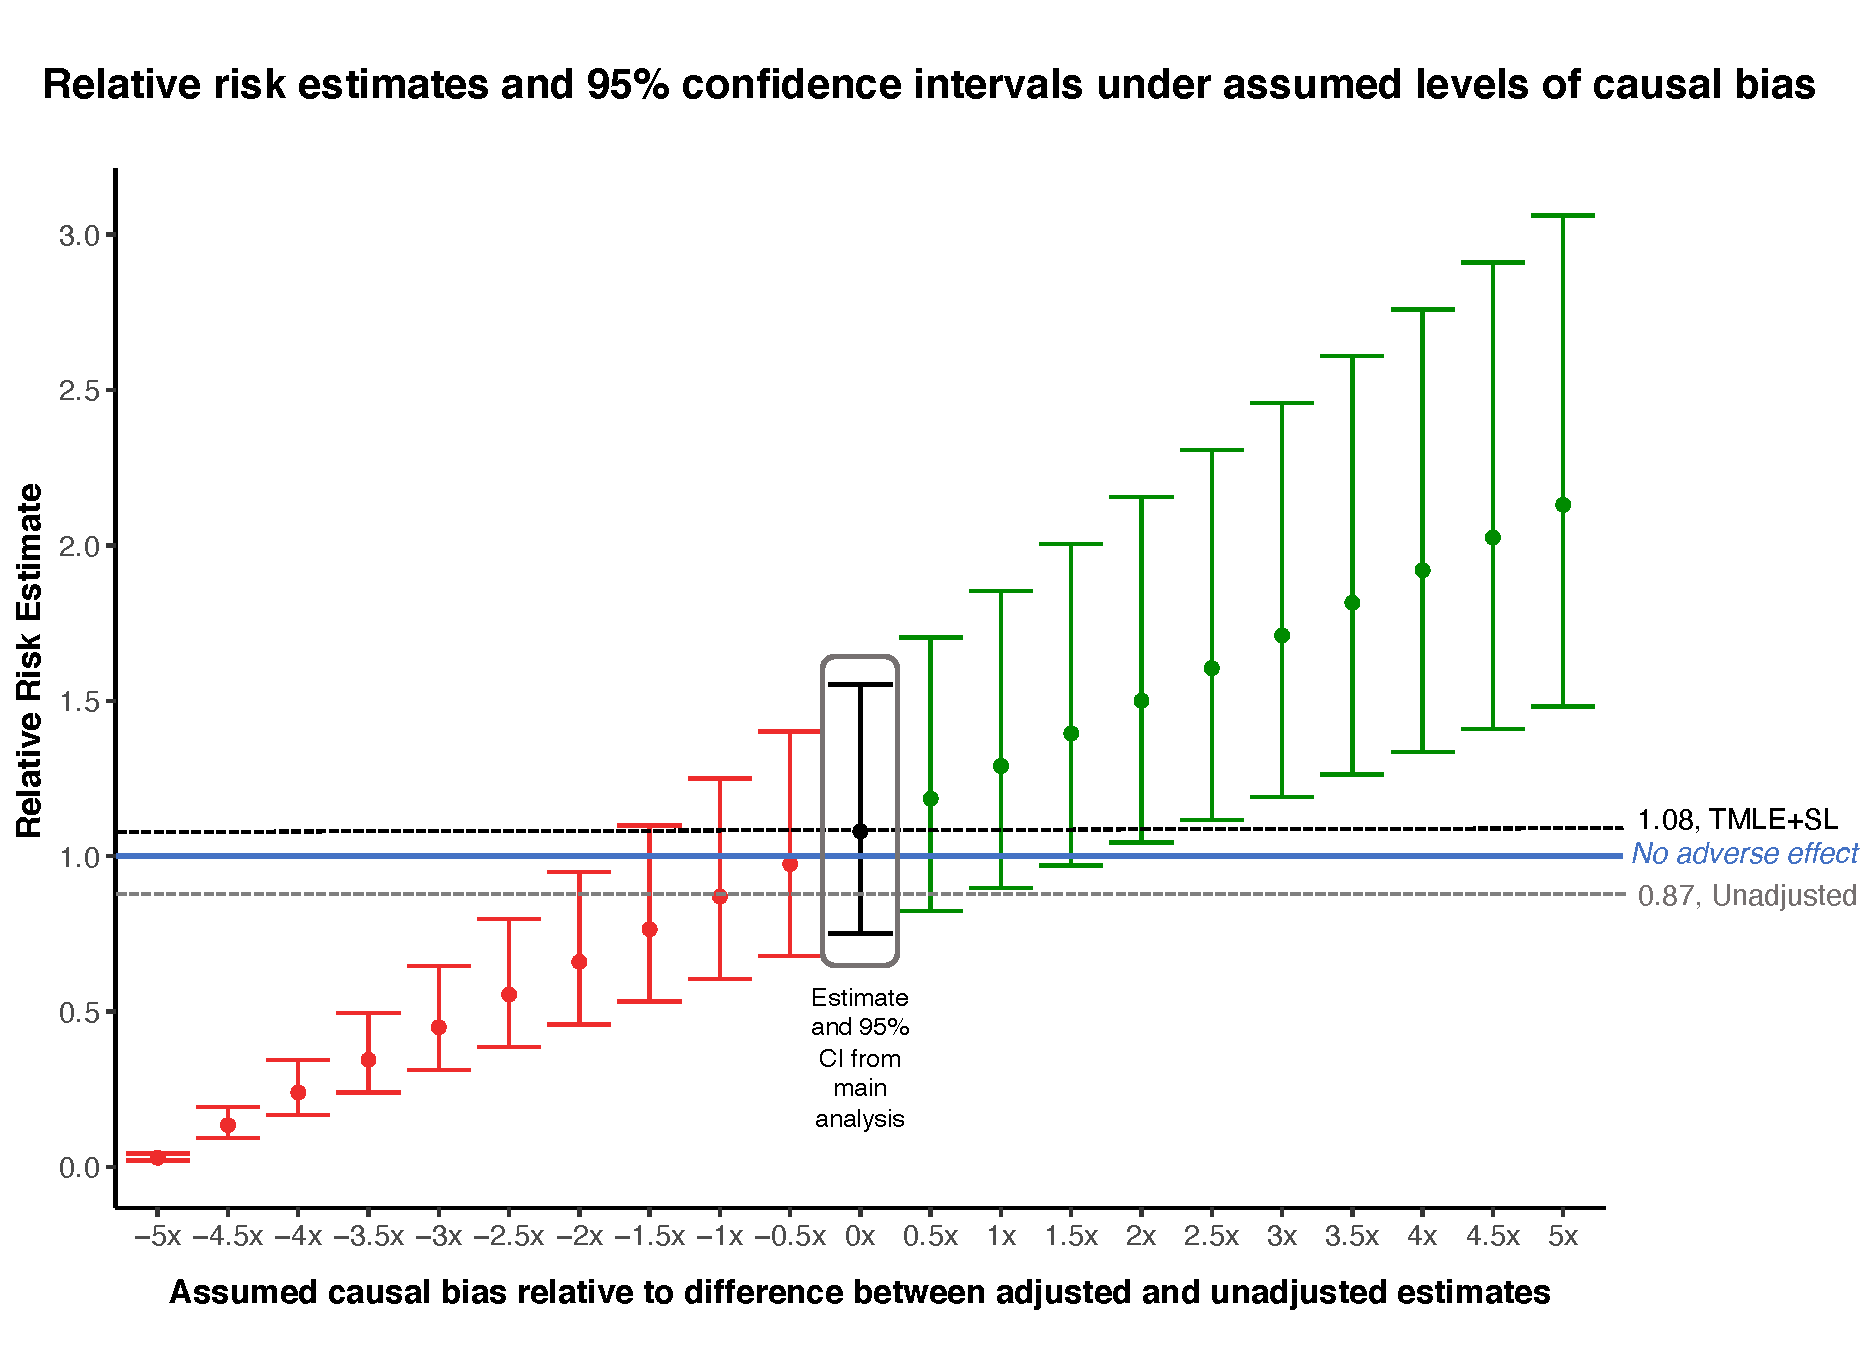
\includegraphics[width = 1.01\textwidth]{figures/sens_plot.pdf}
  \end{center}
\end{frame}


%\section{Targeted Learning with RWD}

\begin{frame}
\frametitle{Targeted Learning with RWD}
\vspace{-18pt}
\centering
\begin{figure}
\begin{center}
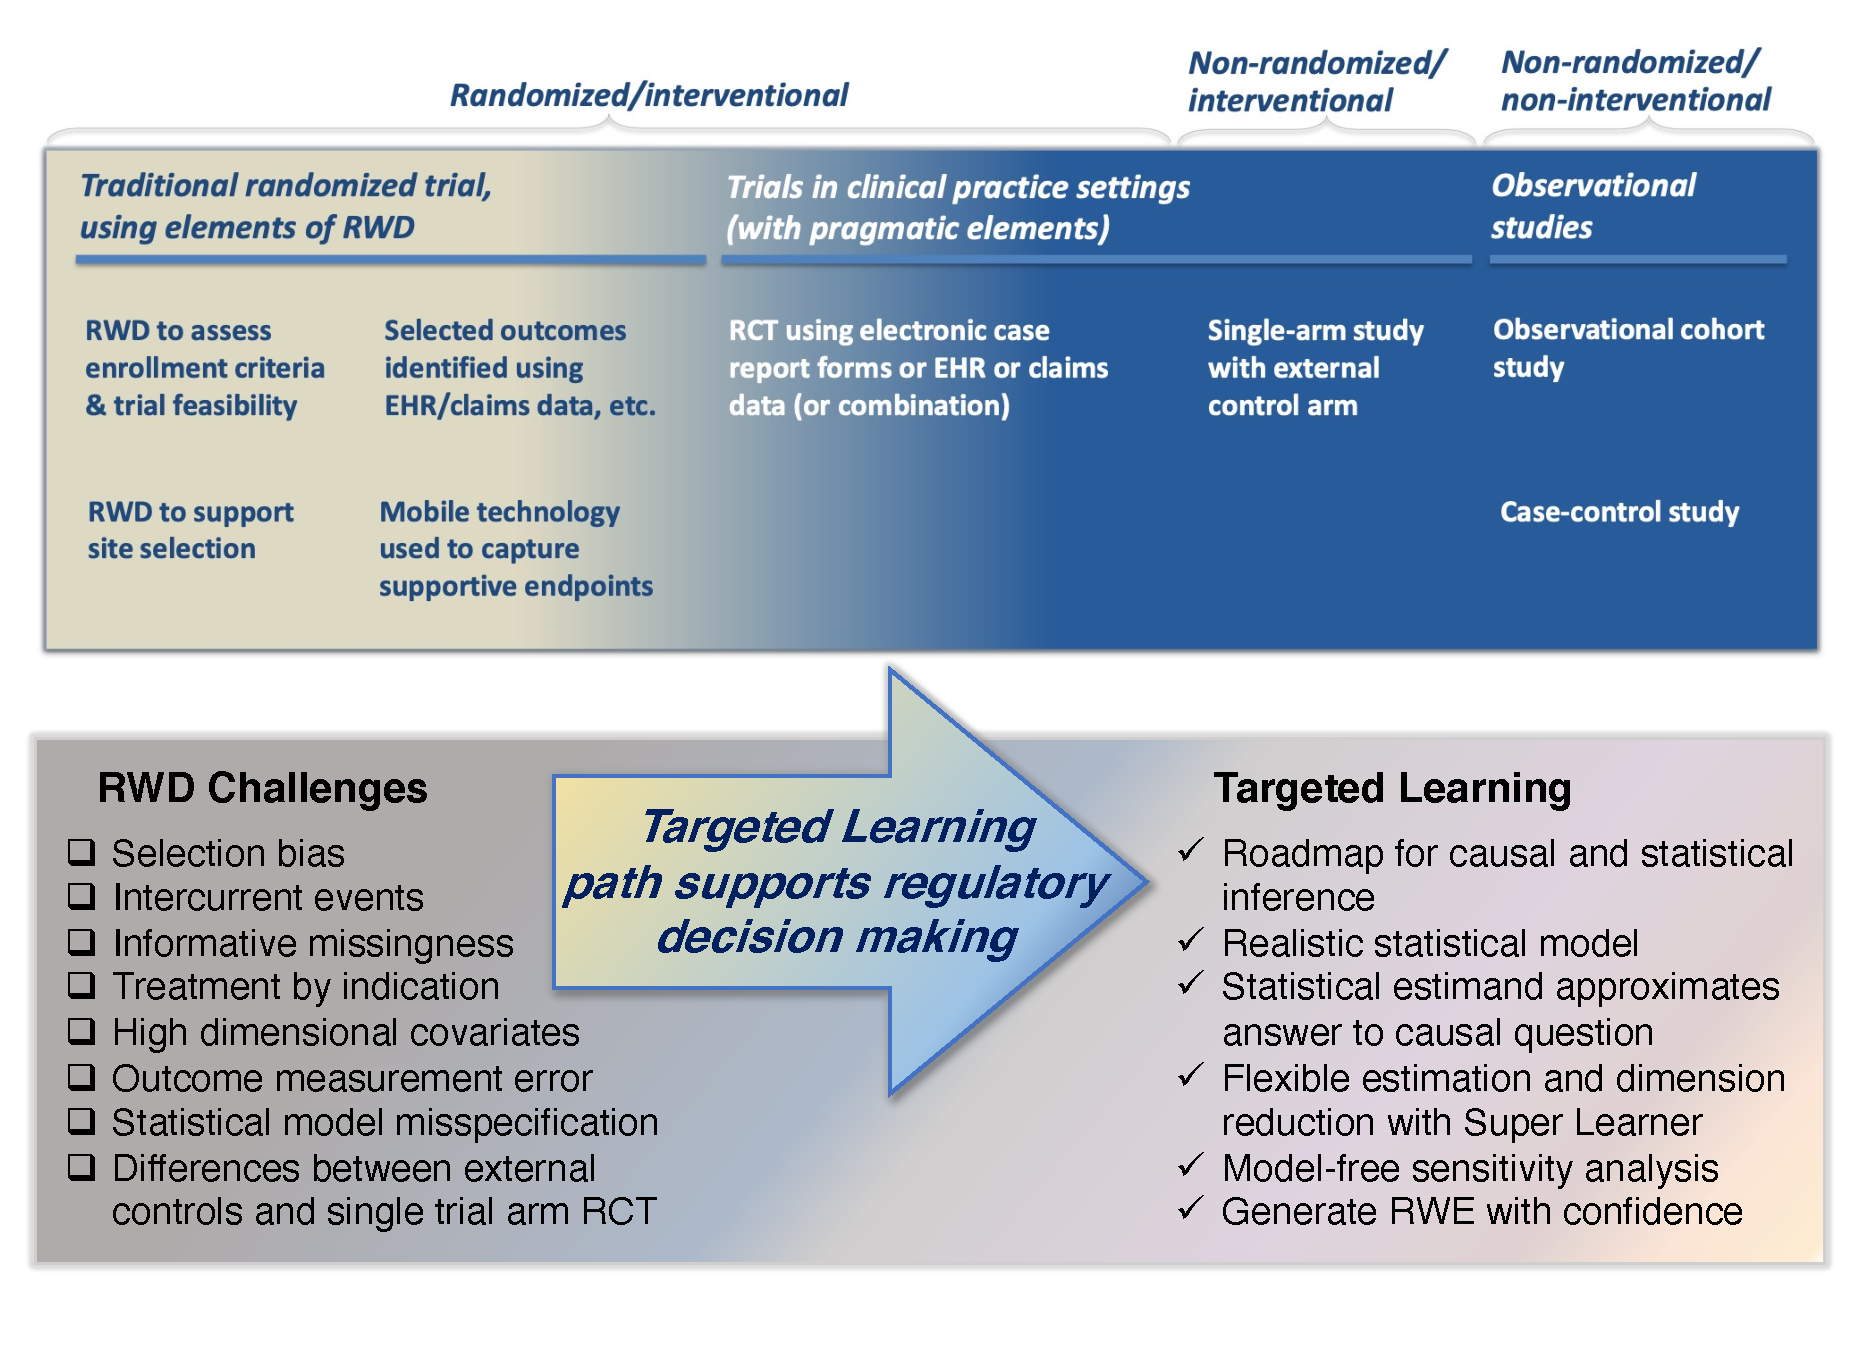
\includegraphics[width=1.02\textwidth]{figures/TLpath2_edit.pdf}
\end{center}
\end{figure}
\vspace{35pt}
\end{frame}

\section{TL in longitudinal RW studies}
%can we add causal graph picture
\begin{frame}
\frametitle{General Longitudinal Data Structure for Complex Observational Studies}
We observe $n$ i.i.d. copies of a longitudinal data structure
\[
O=(L(0),A(0),\ldots,L(K),A(K),Y=L(K+1)),\]
where $A(t)$ denotes a discrete valued {\bf intervention node} whose effect we desire to evaluate,  $L(t)$ is an intermediate covariate and outcome realized in between intervention nodes $A(t-1)$ and $A(t)$, $t=0,\ldots,K$, and $Y$ is a final {\bf outcome} of interest.
\ \newline
{\bf Survival outcome example:}
For example, 
\begin{eqnarray*}
A(t)&=&(A_1(t),A_2(t))\\
A_1(t)&=& \mbox{Indicator of being treated at time $t$}\\
A_2(t)&=& \mbox{Indicator of being right-censored at time $t$}\\
%\Delta&=&\mbox{Indicator of observing failure}\\
Y(t)&=&\mbox{Indicator of observing a failure by time $t$}\\
L(t)&&\mbox{Vector of time-dependent measurements}\\
Y(t)&\subset& L(t)\mbox{and  $Y=Y(K+1)$}.
\end{eqnarray*}
\end{frame}


% \subsection{Targeted learning in complex observational study of diabetes (Neugebauer et al.)}

\begin{frame}{A real-world CER study comparing different rules for treatment intensification for diabetes}
\begin{itemize}
\item Data extracted from diabetes registries of 7 HMO research network sites: 
\begin{itemize}
\item Kaiser Permanente
\item Group Health Cooperative 
\item HealthPartners
\end{itemize}
%\end{itemize}
%\end{frame}
%\begin{frame}
%\begin{itemize}
\item  {\bf Enrollment period:} Jan 1$^{\textrm{st}}$ 2001 to Jun 30$^{\textrm{th}}$ 2009
%\item Patients enrolled the first time treatment intensification (TI) was first indicated as long as the benefits and harms of TI were unclear.
\end{itemize}
 {\bf Enrollment criteria:} \\ 
\vspace{-0.2cm}\begin{itemize}
\item past A1c$<7\%$ (glucose level) while on 2+ oral agents or basal insulin 
\item $7\%\leq$ latest A1c $\leq 8.5\%$  (study entry when glycemia was no longer reined in)
\end{itemize}
\end{frame}
\begin{frame}{Longitudinal data}

\begin{itemize}
\item {\bf Follow-up} til the earliest of Jun 30$^{\textrm{th}}$ 2010, death, health plan disenrollment, or the failure date
\item {\bf Failure} defined as onset/progression of albuminuria (a microvascular complication) 
\item {\bf Treatment} is the indicator being on ''treatment intensification'' (TI)
\item $n\approx 51,000$ with a median follow-up of 2.5 years.
\item {\bf Target estimand:} What would survival look like if treatment is intensified when $A1c<x\%$ for various levels $x=7,7.5,8,8.5$?
\end{itemize}
\end{frame}

\begin{frame}
\frametitle{Likelihood and Statistical Model}
The probability density/likelihood $p_0$ of $O$ can be {\bf factorized according to the time-ordering} as 
\begin{eqnarray*}
p_0(O)&=&\prod_{t=0}^{K+1} p_0(L(t)\mid Pa(L(t)) ) \prod_{t=0}^K p_0(A(t)\mid Pa(A(t)) )\\
&\equiv& \prod_{t=0}^{K+1}q_{0,L(t)}(O)\prod_{t=0}^K g_{0,A(t)}(O)\\
&\equiv& q_0g_0,
\end{eqnarray*}
where $Pa(L(t))\equiv (\bar{L}(t-1),\bar{A}(t-1))$ and $Pa(A(t))\equiv (\bar{L}(t),\bar{A}(t-1))$ denote the parents  of $L(t)$ and $A(t)$ in the time-ordered sequence, respectively. 
The $g_0$-factor represents the {\bf intervention mechanism}.\newline
{\bf Statistical Model:}
We make no assumptions on $q_0$, but could make assumptions on $g_0$.
\end{frame}


\begin{frame}
\frametitle{Statistical Target Parameter: $G$-computation Formula for Post-dynamic-Intervention Distribution}
\begin{itemize}
\item $p^{g^*}_0=q_0(o)g^*(o)$ is the {\bf $G$-computation formula for the post-intervention distribution} of $O$ under the stochastic intervention $g^*=\prod_{t=0}^K g^*_{A(t)}(O)$.
\item Under {\bf sequential randomization assumption} (SRA) and a positivity assumption, the post-intevention distribution $p_{g^*}$ of $O$ equals $p_{g^*}$, where post-intervention distribution is defined by the structural equation model in which the equations for the intervention nodes $A(t)$ are replaced by drawing from $g^*_{A(t)}$.
\item {\bf Causal estimand}: $E_{P_{g^*}}Y$, mean outcome of $Y$ under post-intervention distribution, or survival rate if $Y$ is indicator of survival, under  post-intervention $P_{g^*}$.
\item {\bf Target estimand}: $E_{P^{g^*}}Y$, mean outcome of $Y$ under $G$-computation density.
%\itemIn particular, for a dynamic intervention $d=(d_t: t=0,\ldots,K)$ with $d_t(\bar{L}(t),\bar{A}(t-1))$ being the treatment at time $t$, the $G$-computation formula is given by \begin{align*}\label{eqn:Gcomp}p^d_0(l)=\prod_{t=0}^{K+1}q_{0,L(t)}^d(\bar{l}(t)),\end{align*}
%Susan: replace 1 by bar{a}(k-1)where $q_{L(t)}^d(\bar{l}(t))=q_{L(t)}(l(t)\mid \bar{l}(t-1),\bar{A}(t-1)=\bar{d}_{t-1}(\bar{l}(t-1)) )$. \itemLet $L^d=(L(0),L^d(1),\ldots,Y^d=L^d(K+1))$ denote the random variable with probability distribution $P^d$. 
%\item This is the so called $G$-computation formulafor the post-intervention distribution corresponding with the dynamic intervention $d$.
%It is naturally generalized to the post-intervention distribution for stochastic interventions defined by user-supplied choice $g^*$. 
\end{itemize}
\end{frame}

\begin{frame}
\frametitle{Better clinical decisions from observational data}
\vspace{-20pt}
\begin{center}
  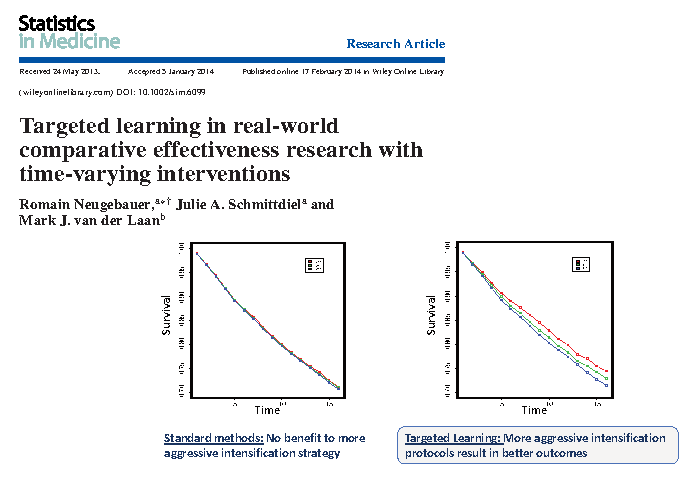
\includegraphics[width = 1.02\textwidth]{diabetes.pdf}
  \end{center}
\end{frame}


%\begin{frame}{Using longitudinal TMLE to estimate treatment-rule-specific survival curves}
%  \frametitle{Super learning: data demonstration}\vspace{-.1in} \begin{figure}  \includegraphics[width=1.0\textwidth]{mayaslides/Presentation1.pdf}
%  \includegraphics[width=1.0\textwidth]{mayaslides/slide09.jpg}  \end{figure} \end{frame}

\section{SL and Variable Importance Analysis with INFORM}

\begin{frame}{Predicting risk for COVID-19 infection, hospitalization or death}

\begin{itemize}
\item For any subject in study, define $t=0$ as January 2022: one might consider other $t=0$ times individualized by an enrollment criterion).
\item $K+1$ is {\bf number of months of follow up} after $t=0$ at which we want the outcome $Y$  of interest.
\item $L(0)$ represents {\bf baseline history} for this subject, including any past events, medical history etc.
\item Define as {\bf intervention nodes} $A(t)$ indicator of being censored by time $t$ (e.g. death by other causes, end of study).
%\end{itemize}\end{frame}\begin{frame}\begin{itemize}
\item Define {\bf outcome} $Y$ as the indicator of observing a COVID-19 infection by time  $t=K+1$.
\item Define {\bf time-dependent covariates} $L(t)$ as anything observed in month $t$, before $A(t)$: including COVID-19 Infection/Hospitalization/Death, vaccination, medical treatments etc.
\end{itemize}
\end{frame}
\begin{frame}
\begin{itemize}
\item Our target is $E(Y_{\bar{a}=0}\mid L(0))$: {\bf conditional risk of COVID-19 infection by time $K+1$ in counterfactual world without right-censoring}. 
\item So our goal is to predict risk of COVID-19 event by $K+1$-months in world without right-censoring. 
\item One  may look at various {\bf other outcomes} of interest such as hospitalization, death, composite outcomes etc. 
\end{itemize}
\end{frame}

\begin{frame}{Super-learner to Predict COVID-19 Risk from baseline information}
\begin{itemize}
\item One can set up a collection of logistic regression machine learning algorithms, including a variety of HAL-model fits.
\item One has to select a {\bf measure of performance}, such as AUC, log-likelihood, or MSE.
\item To deal with drop-out (right-censoring), we can use {\bf inverse probability of censoring weights} for each candidate algorithm and for evaluating the cross-validated performance of the algorithm.
% more sophisticated alternative is sequentially double robust sequential machine learning (Luedtke et al. )
\item The super-learner will output the best performing prediction function, its measure of performance (e.g., AUC) with a confidence interval. 
\end{itemize}
\end{frame}

\begin{frame}{Variable importance analysis using TMLE}
\begin{itemize}
\item Let $W=L(0)$.
\item One has to {\bf define a measure of importance} for each variable $W_j$. 
\item For example, for {\bf binary} $W_j$, one can use the {\bf ATE} estimand, which measures change in prediction due to $W_j=0$ versus $W_j=1$ keeping $W(-j)$ constant.
\item For {\bf continuous} $W_j$ one can use the {\bf shift-intervention} estimand, which measures change in prediction due to shifting  $W_j$ to $W_j+\delta$, keeping $W(-j)$ constant.
\item One can compute TMLE of these $W_j$-specific variable importance measures, with confidence intervals and $p$-values.
\item One can use {\bf multiple testing adjustments} to control family wise error or false discovery rate.
\end{itemize}
\end{frame}

%\section{Variable importance analysis examples of Targeted Learning}

\begin{frame}{Example 1: Predicting Death for Trauma Patients in ICU}
\begin{itemize}
\item Around 800 patients that entered the emergency room with severe
  trauma
\item About 80 physiological and clinical variables were measured at 0,
  6, 12, 24, 48, and 72 hours after admission
\item Objective is predicting the most likely medical outcome of a
  patient (e.g., survival), and provide an ordered list of the covariates that drive  this prediction (variable importance).
\item This will help doctors decide what variables are relevant at
  each time point.
  % Intervention is not observing any other variables?
\item Variables are subject to missingness
\item Variables are continuous, variable importance parameter is
\[\Psi(P_0)\equiv E_0\{E_0(Y\mid A+\delta,W)-E_0(Y\mid A,W)\}\]
for user-given value $\delta$.
\end{itemize}
\end{frame}

\begin{frame}{Example I: Variable Importance results}
\begin{figure}[H]
\includegraphics[width=150pt]{eff1.pdf}
\caption{Effect sizes and significance codes}
\end{figure}
\end{frame}


\begin{frame}{Example II: Predicting Spina Bifida from Genomic Data}
\begin{itemize}
\item 570 case-control samples on spina bifida
\item We want to identify associated genes to spina bifida from 115 SNPs.
\item In the original paper Shaw et. al. 2009, a univariate analysis was
performed.
\end{itemize}
\end{frame}
%\begin{itemize}\item The original analysis missed rs1001761 and rs2853532 in TYMS genebecause they are closely linked with counteracting effects on spinabifida.\item With TMLE, signals from these two SNPs were recovered.\item In TMEL, Q0 was obtained from LASSO, and $g(W)$ is obtained from asimple regression of SNP on its two flanking markers to account forconfounding effects of neighborhood markers.\end{itemize}\end{frame}



%\begin{frame}{TMLE Result}\begin{center}\begin{tabular}{cccccc}\toprule       & \multicolumn{2}{c}{Effect estimate}  &&\multicolumn{2}{c}{P-value} \\\hline \\        & rs1001761 & rs2853532   	&&  rs1001761 	& rs2853532  \\\cmidrule{2-3} \cmidrule{5-6}UR     & -0.08	 & -0.02		&&	4.5x10$^{-3}$	&5.0x10$^{-1}$ \\		TMLE   & -0.18	 &  0.09	      &&	4.0x10$^{-5}$	&2.5x10$^{-2}$ \\\bottomrule \end{tabular}

\begin{frame}{Example II: Variable importance results}
TMLE p-values for SNPs
\includegraphics[height=0.5\textwidth,
width=1\textwidth]{result_tmle_lm.pdf}

%\end{center}

\end{frame}

\begin{frame}{Example III: Predicting Health Spending from Medical Conditions}
\begin{figure}
\vspace{-2pt}
\includegraphics[width=200pt]{result2crop.pdf}
%\includegraphics[height=3.1in]{result2crop.pdf}
\end{figure}
\tiny{Rose (2016). Robust targeted machine learning for variable importance in health spending.}
\end{frame}

%\begin{frame}{Implications}First investigation of the impact of medical conditions on health spending as a variable importance question using TMLE.\begin{block}{}Five most expensive medical conditions were \begin{enumerate}\item multiple sclerosis\item congestive heart failure\item lung, brain, and other severe cancers\item \textbf{major depression and bipolar disorders}\item \textbf{chronic hepatitis.}\end{enumerate}\end{block}\begin{itemize}\item Differing results compared to parametric regression.\item What does this mean for incentives for prevention and care?\end{itemize}\end{frame}

\section{Causal Inference with INFORM}

\begin{frame}{Causal inference with INFORM: Causal impact of COVID-19 on overall care/cost/health etc}
\begin{itemize}
\item Suppose we are interested in causal impact of {\bf COVID-19 infection} in the first time window on  $Y(K+1)$, such as number of missed planned hospital visits by time $K+1$.  
\item One might then define $A(0)$ as the indicator of having a COVID-19 infection in the first time window after baseline. 
\item One can define $A(t)$ as the indicator of being right-censored in $t$-th time window: $t=1,\ldots,K$. 
%\item One can define $Y$ as the number of missed hospital visits.
\item One might be interested in the {\bf Average Treatment Effect} of $A(0)$ on $Y$:
\[
E(Y_{1}-Y_0),\]
where $Y_0,Y_1$ denotes the counterfactual indicator of death when COVID-10-infection is 
withhold,enforced at time $0$, in a world in which there is no right-censoring.
\end{itemize}
\end{frame}
\begin{frame}{Optimal subgroup to target for prevention of COVID-19 w.r.t. cost/health, under resource constraints}
\begin{itemize}
\item One could also estimate the conditional causal effect (CCE) $E(Y_1-Y_0|W)$  given individual characteristics $W$ (including IC etc): Highly Adaptive Lasso, combined with inference.
\item The CCE implies an optimal individualized COVID-prevention strategy $W\rightarrow d(W)\in \{0,1\}$ for optimizing future cost/health or other key outcomes,  under resource constraints: order CCE and first prevent COVID for individuals with largest gains. 
\item In addition, given an estimate $d_n(W)$ of this optimal COVID-prevention rule, we can obtain inference for the population level outcome $EY_{d_n(W)}$ when applying this prevention rule $d_n$ to our target population. 
\item In addition, we can evaluate population level outcome under different candidate rules. 
\end{itemize}
\end{frame}
\begin{frame}{TMLE for average causal impact of single time point and multiple time-point interventions on COVID-19 infection}
\begin{itemize}
\item We could use the TMLE of ATE earlier presented, using inverse probability of censoring weighting. Or we can use the longitudinal TMLE (ltmle()).
\item One can also evaluate impact of {\bf time at  COVID-19-infection}  onto overall care $Y$ missed. In that case, one can define $A_1(t)$ as indicator of having a COVID-19-infection by time $t$ and consider {\bf counterfactual overall care outcomes}  such as (say for three time points) $Y_{100}, Y_{010}, Y_{001}$.
\item The {\bf causal estimand} would be counterfactual mean overall care, $EY_{\bar{a}_1}$, for these regimens $\bar{a}_1$ that show a jump at a particular time $t(\bar{a}_1)$. One could summarize this curve with a {\bf marginal structural working model} such as $EY_{\bar{a}_1}=\beta_0+\beta_1 t(\bar{a}_1)$ so that $\beta_1$ represents the (average) additive causal effect on overall care $Y$ due to  shifting the time at COVID-19  infection by one unit.
\end{itemize}
\end{frame}
\begin{frame}\begin{center}
THANK YOU!
\end{center}
\end{frame}

%\section{Towards TL in FDA-safety analysis)}

%\begin{frame}{FDA Funded Demonstration Project}FDA has funded a two year demonstration project of TL (led by Susan Gruber) involving \begin{itemize}\item Simulations imitating real world studies demonstrating the roadmap and showcasing that TMLE outperforms propensity score matching and  other current methods of choice.\item Weekly meetings with senior FDA statisticians and us (S. Gruber, Rachael Philips, MvdL).\item Monthly meetings updating the leadership of real world analytics group at FDA.\item Workshop on TL at FDA\item Publications of various articles reporting on findings.\item Regular seminars on topics in TL, recorded and  made public.\item Educational short videos on key concepts in TL.\end{itemize}\end{frame}



%\begin{frame}{FDA funded Sentinel Innovation Center on Causal inference with Real World Data}\begin{itemize}\item Sentinel is the FDA national electronic system transforming the way researchers monitor the safety of FDA-regulated medical products. Launched in response to FDA Amendments Act of 2007. \item Innovation Center  is  led by Department of Pharmacoepidemiology  of Harvard University\item Working group includes FDA, Pharma, and academic statisticians. \item Full focus on how to apply TL to real world data sets in Sentinel system, and evaluating its performance relative to other approaches. \end{itemize}\end{frame}

%\begin{frame}{Using Innovation Center to showcase how to set up TL Statistical Analysis Plan (SAP) }\begin{itemize}\item Specification of a TMLE relies on various choices that can be tailored towards precise application in question: e.g., library of super-learner; truncation method; type of TMLE, e.g., collaborative  TMLE or not. \item We use outcome blind version of data set in question to set  up simulation of (similar) data sets for which we know the truth.\item We then then select a TMLE that performs best w.r.t. coverage of 0.95 confidence intervals, bias and mean squared error, optimizing power while controlling type-I error and coverage. \item Results demonstrate for particular rare outcome diseases that C-TMLE is superior thereby providing the choice of SAP, which will then be applied to real data (Reference: Wijss et al., 2023)\end{itemize}\end{frame}

%\section{Adaptive Designs}\begin{frame}\frametitle{Robust inference for adaptive sequential RCTs}
%  \frametitle{Performance of the ``best'' subset rule}
%  \frametitle{Adaptive randomization for sequential RCTs}\vspace{-15pt}\centering  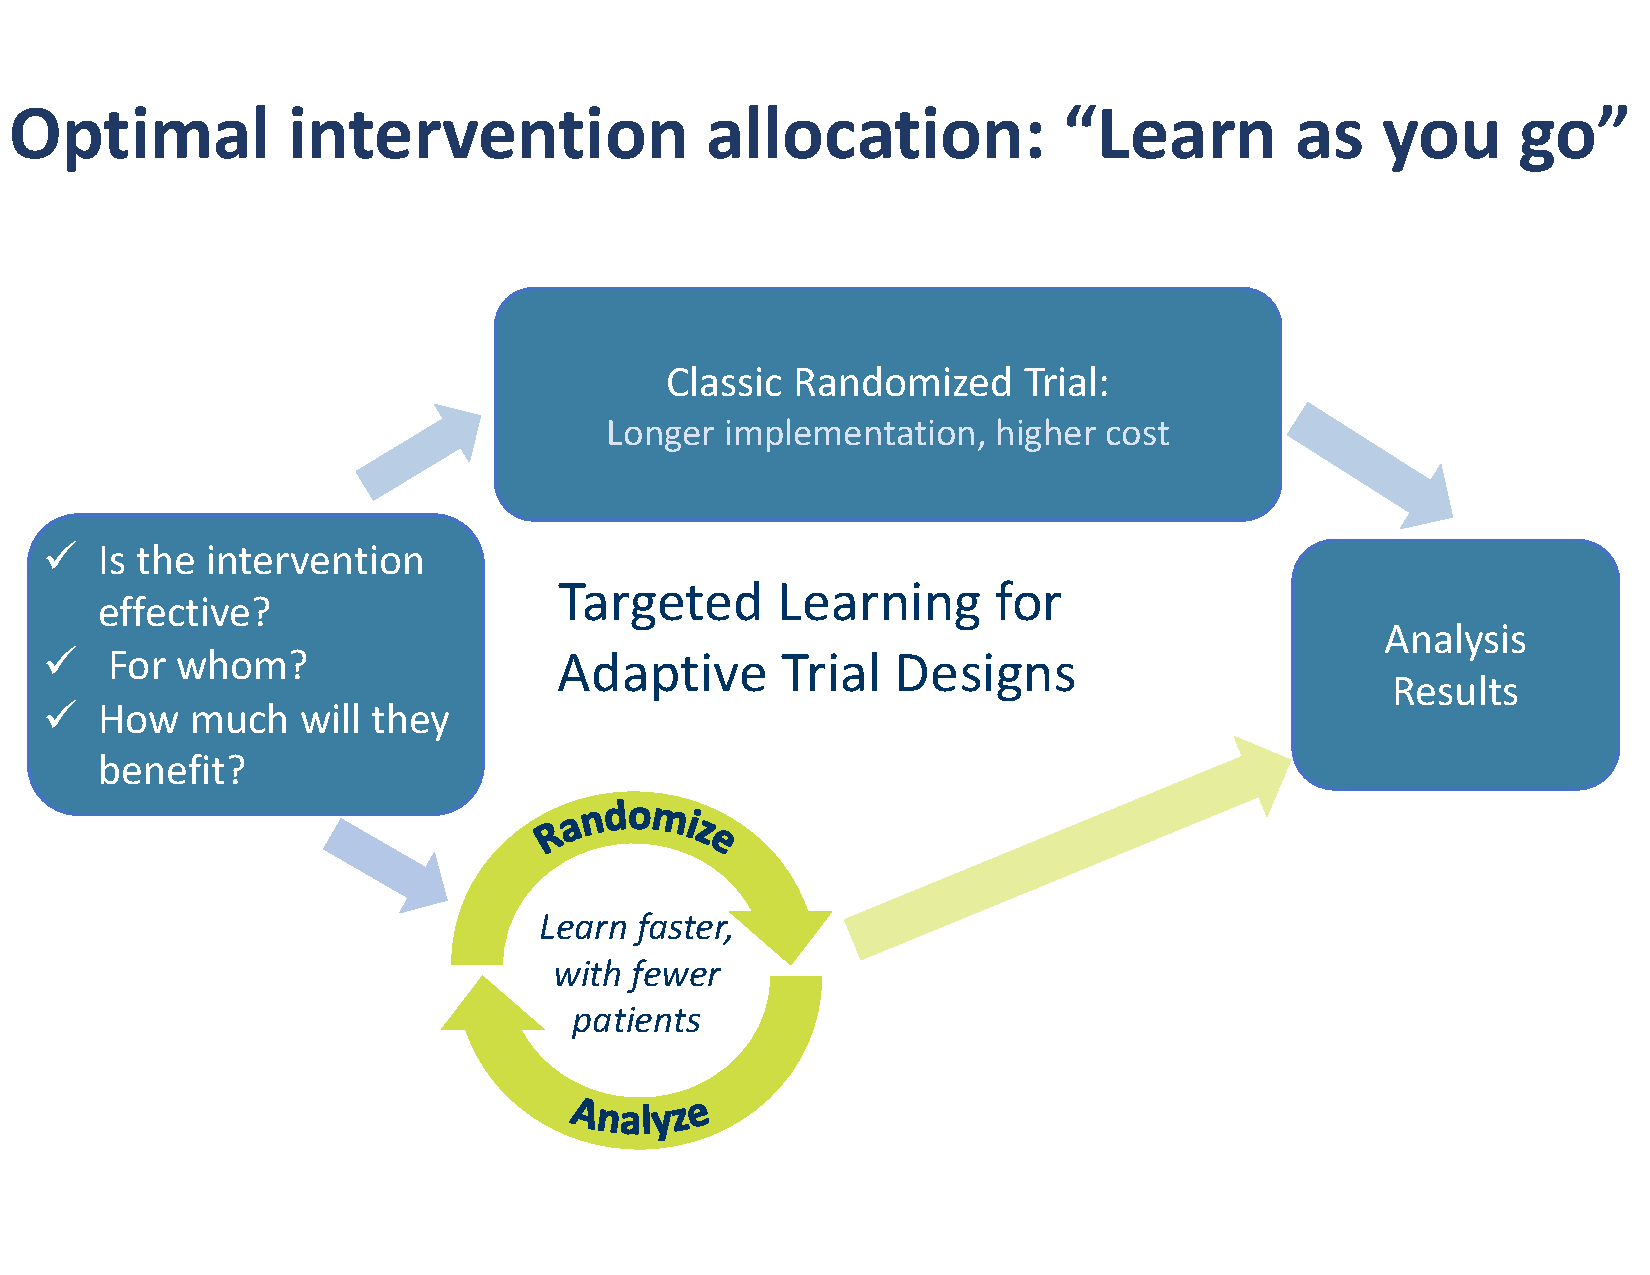
\includegraphics[scale=0.35]{learnasyougo_cropped.pdf}\end{frame}


% \begin{frame}
% \frametitle{Adapting the randomization probabilities in a sequence of Sepsis RCTs}
% \begin{itemize}
%     \item We sequentially draw 8 blocks of 100 observations $(W_i,A_i,Y_i)$, $W$ including adrenal insufficiency (binary); serum levels.
%     \item At each block, we use {\bf super learning of optimal rule} and TMLE to estimate its {\bf counterfactual death rate}. 
%   % \item For the adaptive design we then set the randomization probabilities for next block accordingly, while balanced design keeps flipping coin when assigning treatment.
%     \item We report performance of the fixed balanced design and the adaptive design learning the optimal rule w.r.t.  {\bf percentage receiving optimal rule}; observed {\bf death rate}; {\bf coverage} of confidence  intervals.
%     \end{itemize}
%     \end{frame}

%\begin{frame}\frametitle{Balanced vs. adaptive sequential design}\centering\animategraphics[autoplay,loop,width=0.8\linewidth]{10}{Survival_PercentSamples/gganim_plot}{0001}{0100}\end{frame}\begin{frame}\frametitle{Balanced vs. adaptive sequential design}\vspace{-5pt}\begin{figure}%    \centering
    %\caption{Width of the Confidence Interval and Percent Death in Balanced and Adaptive Sequential Trial}%    \subfloat{{\animategraphics[autoplay,loop,width=0.49\linewidth,height=0.49\linewidth]{10}{Survival_WidthCI/gganim_plot}{0001}{0100} }}%
    %\qquad    \subfloat{{\animategraphics[autoplay,loop,width=0.49\linewidth,height=0.49\linewidth]{10}{Survival_MeanOutcome/gganim_plot}{0001}{0100} }}%
    %\label{fig:example}%\end{figure}\end{frame}

%\begin{frame}\frametitle{Ongoing applications with Targeted Learning}\begin{itemize} \item Causal inference with survival and competing risk time to event outcomes. \item Sequential adaptive RCTs (self-learning systems).    \item Online learning from wearable devices   \item Causal inference for networks: When one person treatment affects another person's outcome   \item Causal inference for time series (e.g., RCT within a single individual).   \item Learning from EHR data with  better confounder control (incorporating NLP).\item Causal inference in continuous time.\end{itemize}\end{frame}

\end{document}

\section{Adaptive Designs}

\begin{frame}
\frametitle{Robust inference for adaptive sequential RCTs}
%  \frametitle{Performance of the ``best'' subset rule}
%  \frametitle{Adaptive randomization for sequential RCTs}
\vspace{-15pt}
\centering
  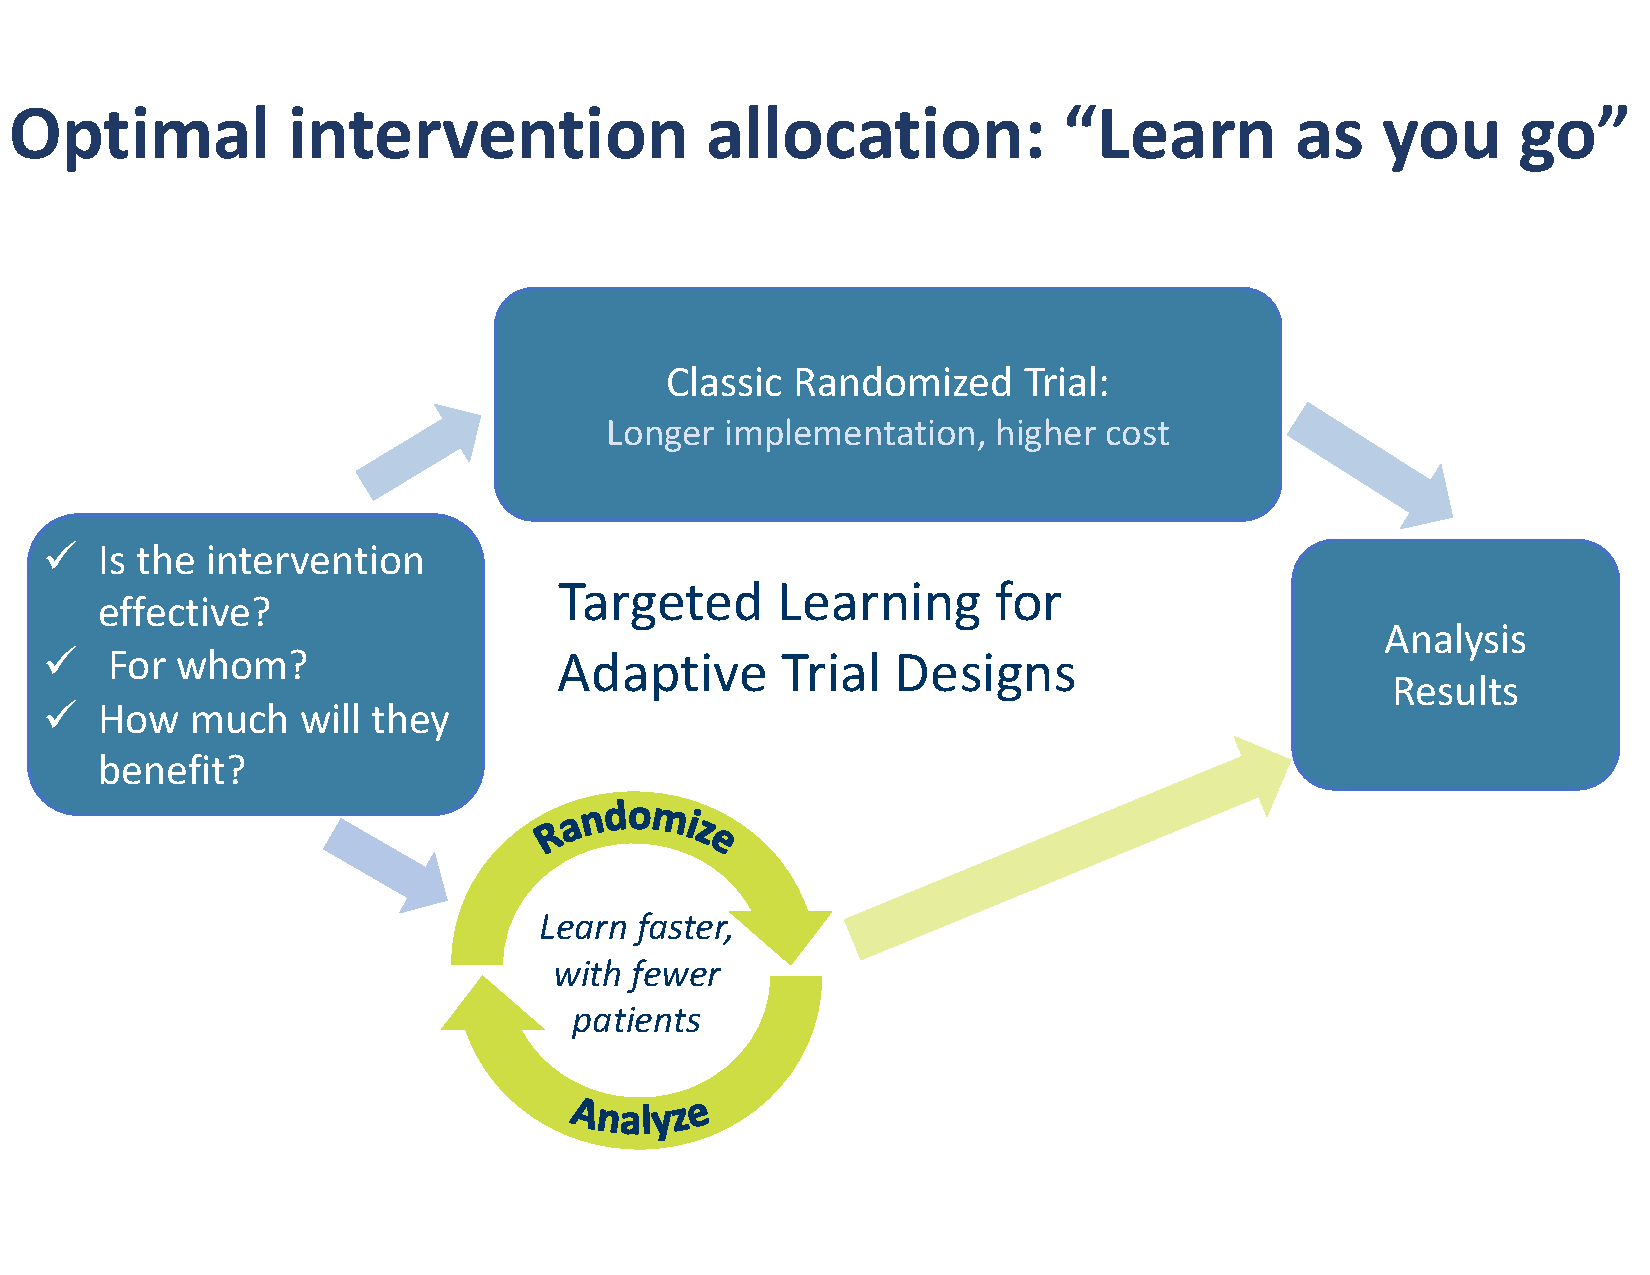
\includegraphics[scale=0.35]{learnasyougo_cropped.pdf}
\end{frame}


% \begin{frame}
% \frametitle{Adapting the randomization probabilities in a sequence of Sepsis RCTs}
% \begin{itemize}
%     \item We sequentially draw 8 blocks of 100 observations $(W_i,A_i,Y_i)$, $W$ including adrenal insufficiency (binary); serum levels.
%     \item At each block, we use {\bf super learning of optimal rule} and TMLE to estimate its {\bf counterfactual death rate}. 
%   % \item For the adaptive design we then set the randomization probabilities for next block accordingly, while balanced design keeps flipping coin when assigning treatment.
%     \item We report performance of the fixed balanced design and the adaptive design learning the optimal rule w.r.t.  {\bf percentage receiving optimal rule}; observed {\bf death rate}; {\bf coverage} of confidence  intervals.
%     \end{itemize}
%     \end{frame}

\begin{frame}
\frametitle{Balanced vs. adaptive sequential design}
\centering
\animategraphics[autoplay,loop,width=0.8\linewidth]{10}{Survival_PercentSamples/gganim_plot}{0001}{0100}
\end{frame}

\begin{frame}
\frametitle{Balanced vs. adaptive sequential design}
\vspace{-5pt}
\begin{figure}%
    \centering
    %\caption{Width of the Confidence Interval and Percent Death in Balanced and Adaptive Sequential Trial}%
    \subfloat{{\animategraphics[autoplay,loop,width=0.49\linewidth,height=0.49\linewidth]{10}{Survival_WidthCI/gganim_plot}{0001}{0100} }}%
    %\qquad
    \subfloat{{\animategraphics[autoplay,loop,width=0.49\linewidth,height=0.49\linewidth]{10}{Survival_MeanOutcome/gganim_plot}{0001}{0100} }}%
    %\label{fig:example}%
\end{figure}
\end{frame}


% \begin{frame}
% \frametitle{Convergence of adaptive randomization probabilities towards optimal rule}
% \vspace{5pt}
% \centering
% \begin{figure}%
% \includegraphics[scale=0.3]{design_convergence}
% \end{figure}
% \end{frame}


% \begin{frame}{TMLE-based statistical inference for performance under current best estimate of rule}
% \vspace{15pt}
%     \includegraphics[scale=0.3]{adaptive_design_inference}
% \end{frame}
% \subsection{Complex Observational Studies}

% \begin{frame}
% \frametitle{Longitudinal data structure}
% We observe $n$ i.i.d. copies of a longitudinal data structure
% \[
% O=(L(0),A(0),\ldots,L(K),A(K),Y=L(K+1)),\]
% where 
% \begin{itemize}
%     \item $A(t)$ denotes a discrete valued {\bf intervention node} whose effect we desire to evaluate
%     \item $L(t)$ is an {\bf intermediate covariate/outcome} realized in between intervention nodes $A(t-1)$ and $A(t)$, $t=0,\ldots,K$
%     \item $Y$ is the {\bf final outcome} of interest
% \end{itemize}    
% \end{frame}
% \begin{frame}
% \frametitle{Survival outcome example}
% \begin{eqnarray*}
% A(t)&=&(A_1(t),A_2(t))\\
% A_1(t)&=& \mbox{Indicator of being treated at time $t$}\\
% A_2(t)&=& \mbox{Indicator of being right-censored at time $t$}\\
% %\Delta&=&\mbox{Indicator of observing failure}\\
% Y(t)&=&\mbox{Indicator of observing a failure by time $t$}\\
% L(t)&=&\mbox{Vector of time-dependent measurements}\\
% Y(t)&\subset& L(t) \mbox{and  $Y=Y(K+1)$}.
% \end{eqnarray*}
% \end{frame}

% \begin{frame}
% \frametitle{Likelihood and statistical model}
% The probability distribution $P_0$ of $O$ can be factorized according to the time-ordering as 
% \begin{eqnarray*}
% p_0(O)&=&\prod_{t=0}^{K+1} p_0(L(t)\mid Pa(L(t)) ) \prod_{t=0}^K p_0(A(t)\mid Pa(A(t)) )\\
% &\equiv& \prod_{t=0}^{K+1}q_{0,L(t)}(O)\prod_{t=0}^K g_{0,A(t)}(O)\\
% &\equiv& q_0g_0,
% \end{eqnarray*}
% {\footnotesize
% where $Pa(L(t))\equiv (\bar{L}(t-1),\bar{A}(t-1))$ and $Pa(A(t))\equiv (\bar{L}(t),\bar{A}(t-1))$ denote the parents of  $L(t)$ and $A(t)$, respectively. 

% The $g_0$-factor represents the intervention mechanism.}

% \vspace{15pt}

% {\bf Statistical Model:}
% We make no assumptions on $q_0$, but could make assumptions on $g_0$.
% \end{frame}

% \begin{frame}
% \frametitle{Target estimand}
% \begin{itemize}
% \item $p^{g^*}_0=q_0(o)g^*(o)$ is the $G$-computation formula for the post-intervention distribution of $O$ under the stochastic intervention $g^*=\prod_{t=0}^K g^*_{A(t)}(O)$.

% \vspace{20pt}

% \item Target estimand $\Psi(P)=E_{P_{g^*}}Y$, i.e.,  mean outcome under $P_{g^*}$. 
% \end{itemize}
% \end{frame}


